% ============================================================
%  Adjunction and Irreversibility: From Continuous Fields
%  to Discrete Histories
%  Author: Flyxion
%  Compiled with LuaLaTeX
% ============================================================
\documentclass[12pt, oneside]{memoir}

% ── Fonts ────────────────────────────────────────────────────
\usepackage[T1]{fontenc}
\usepackage[utf8]{inputenc}
\usepackage[sc,osf]{mathpazo}
\linespread{1.05}

% ── Page geometry ────────────────────────────────────────────
\usepackage[
  top    = 1.25in,
  bottom = 1.25in,
  inner  = 1.25in,
  outer  = 1.0in,
  marginparwidth = 0.75in
]{geometry}

% ── Micro-typography ─────────────────────────────────────────
\usepackage{microtype}

% ── Diagrams and figures ─────────────────────────────────────
\usepackage{tikz}
\usepackage{tikz-cd}
\usepackage{pgfplots}
\pgfplotsset{compat=1.18}
\usetikzlibrary{arrows.meta, calc, decorations.pathreplacing, positioning}

% ── Mathematics ──────────────────────────────────────────────
\usepackage{amsmath, amssymb, amsthm, mathtools}
\usepackage{thmtools}

% ── Theorem environments ─────────────────────────────────────
\declaretheoremstyle[
  headfont   = \bfseries,
  notefont   = \mdseries,
  bodyfont   = \itshape,
  spaceabove = 9pt,
  spacebelow = 6pt
]{thmstyle}

\declaretheoremstyle[
  headfont   = \bfseries,
  notefont   = \mdseries,
  bodyfont   = \normalfont,
  spaceabove = 9pt,
  spacebelow = 6pt
]{defstyle}

\declaretheorem[style=thmstyle, numberwithin=section, name=Theorem]{theorem}
\declaretheorem[style=thmstyle, sibling=theorem, name=Proposition]{proposition}
\declaretheorem[style=thmstyle, sibling=theorem, name=Lemma]{lemma}
\declaretheorem[style=thmstyle, sibling=theorem, name=Corollary]{corollary}
\declaretheorem[style=defstyle,  sibling=theorem, name=Definition]{definition}
\declaretheorem[style=defstyle,  sibling=theorem, name=Assumption]{assumption}
\declaretheorem[style=defstyle,  sibling=theorem, name=Conjecture]{conjecture}
\declaretheorem[style=defstyle,  sibling=theorem, name=Remark]{remark}
\declaretheorem[style=defstyle,  sibling=theorem, name=Example]{example}

% ── Tables ───────────────────────────────────────────────────
\usepackage{booktabs}

% ── Graphics ─────────────────────────────────────────────────
\usepackage{graphicx}
\usepackage{xcolor}
\definecolor{linkblue}{RGB}{20, 60, 120}

% ── Hyperlinks ───────────────────────────────────────────────
\usepackage[
  colorlinks = true,
  linkcolor  = linkblue,
  citecolor  = linkblue,
  urlcolor   = linkblue,
  pdftitle   = {Adjunction and Irreversibility},
  pdfauthor  = {Flyxion}
]{hyperref}
\usepackage{cleveref}

% cleveref names for custom theorem environments
\crefname{theorem}{Theorem}{Theorems}
\crefname{proposition}{Proposition}{Propositions}
\crefname{lemma}{Lemma}{Lemmas}
\crefname{corollary}{Corollary}{Corollaries}
\crefname{definition}{Definition}{Definitions}
\crefname{assumption}{Assumption}{Assumptions}
\crefname{conjecture}{Conjecture}{Conjectures}
\crefname{remark}{Remark}{Remarks}
\crefname{example}{Example}{Examples}
\crefname{chapter}{Chapter}{Chapters}
\crefname{section}{Section}{Sections}

% ── Bibliography handled by thebibliography environment ──────

% ── Chapter/section style (memoir) ───────────────────────────
\chapterstyle{article}
\setsecheadstyle{\large\bfseries}
\setsubsecheadstyle{\normalsize\bfseries\itshape}

% ── Header / footer ──────────────────────────────────────────
\pagestyle{ruled}
\makeevenhead{ruled}{\small\thepage}{}{\small\itshape Adjunction and Irreversibility}
\makeoddhead {ruled}{\small\itshape Flyxion}{}{\small\thepage}

% ── Operators & macros ───────────────────────────────────────
\DeclareMathOperator{\Fix}{Fix}
\DeclareMathOperator*{\argmin}{arg\,min}
\newcommand{\X}{\mathcal{X}}
\newcommand{\Y}{\mathcal{Y}}
\newcommand{\Hcal}{\mathcal{H}}
\newcommand{\OO}{\mathcal{O}}
\newcommand{\PP}{\mathcal{P}}
\newcommand{\A}{\mathcal{A}}
\newcommand{\Ft}{\widetilde{F}}
\newcommand{\Fpath}{\widetilde{F}_{\mathrm{path}}}
\newcommand{\Padm}{\mathcal{P}_{\mathrm{adm}}}
\newcommand{\Xadm}{\mathcal{X}_{\mathrm{adm}}}
\newcommand{\Aadm}{\mathcal{A}_{\mathrm{adm}}}
\newcommand{\Dpth}{\Delta_{\mathrm{path}}}
\newcommand{\Djs}{\mathcal{D}_{\mathrm{JS}}}
\newcommand{\KL}{D_{\mathrm{KL}}}
\newcommand{\nnorm}[1]{\lVert #1 \rVert}
\newcommand{\ip}[2]{\langle #1,\, #2 \rangle}
\newcommand{\bv}{\mathbf{v}}
\newcommand{\aq}{a_q}
\newcommand{\av}{a_v}

% ────────────────────────────────────────────────────────────
\begin{document}

% ── Title page ───────────────────────────────────────────────
\begin{titlingpage}
\vspace*{2cm}
{\centering
  \LARGE\bfseries
  Adjunction and Irreversibility:\\[0.4em]
  \Large\mdseries\itshape
  From Continuous Fields to Discrete Histories\\[2.5cm]
  \normalsize\upshape\bfseries Flyxion\\[0.3em]
  \normalfont\small Independent Researcher\\[3cm]
  \normalsize\upshape\today
\par}
\vfill
{\small\noindent
\textit{Abstract.}\enspace
Irreversibility is not a phenomenological gloss on time-asymmetry; it is a structural
theorem about the non-invertibility of reconstruction.  This monograph develops that
claim rigorously across four interlocking registers.  First, we construct a variational
adjunction between a continuous RSVP field space and a discrete history space, and show
that irreversibility is precisely the generic non-isomorphism of the adjunction unit.
Second, we ground the entropy defect on a Refuse-admissible measurable subspace, so that
entropy production is not defined on an undifferentiated ambient configuration space but
on the constraint-preserving stratum generated by admissible trajectories.  Third, we
prove a defect--dynamics correspondence theorem showing that the three-condition crucible
regime---elevated entropy production, retained mutual information, active transport---is
equivalent to a specific bounded interior of the defect space, strictly separated from
both the stable-attractor and fragmentation extremes.  Fourth, we construct an explicit
coupled lattice example in which two trajectories arrive at identical instantaneous field
values through histories separated by a Refuse event, yet are distinguished by a
path-dependent observable, establishing strong history-dependence of projection in at
least the finite-dimensional surrogate.  The framework subsumes semantic thermodynamic
analogy programmes as special cases while replacing their imported rhetoric with derived
objects.
\par}
\end{titlingpage}

\clearpage
\tableofcontents*
\clearpage

% ============================================================
\chapter{Introduction}
\label{ch:intro}
% ============================================================

\section{The problem of irreversibility in constraint-driven systems}

Classical thermodynamics grounds irreversibility in the second law: entropy of a closed
system does not decrease.  That law, however, is phenomenological.  It describes an
observed asymmetry without identifying what structural property of a dynamical system
forces the asymmetry to hold.  When one passes from physical gases to systems defined by
constraint evolution---cognitive systems resolving contradictions, neural networks
navigating loss landscapes, field theories whose degrees of freedom are coupled to an
explicit entropy channel---the phenomenological ground disappears.  One cannot simply
import Boltzmann's argument, because the relevant state spaces are not ensembles of
indistinguishable particles, and the relevant ``heat'' is not thermal agitation but
structured incompatibility between representational layers.

The central question of this monograph is therefore not \emph{what does irreversibility
look like} in such systems, but \emph{what forces it}.  Our answer is categorical and
variational: irreversibility is the generic non-isomorphism of the unit of an adjunction
between a continuous field space and a discrete history space.  When a continuous
trajectory is discretized and then reconstructed via the best possible inverse procedure,
information is lost unless the discretization map is injective.  Entropy is the
measure-theoretic shadow of that loss.  Phase regimes---stable attractor, crucible,
fragmentation---are dynamically realized regions of the defect space induced by the
adjunction.

\section{Three questions that organize the monograph}

Three questions organize what follows.

\medskip\noindent\textit{What is irreversibility in a system defined by constraint
evolution?}\enspace We answer: irreversibility is the defect of the adjunction unit,
measured by the Jensen--Shannon divergence between the original measure on the
configuration space and the measure reconstructed after passing through the discretization
channel.

\medskip\noindent\textit{How does projection loss arise formally rather than
heuristically?}\enspace We answer: projection loss is the non-identity of the comparison
map $\eta = G \circ \Ft$, where $\Ft$ is the surrogate discretization and $G$ is the
variational reconstruction operator.  Loss is not assumed; it is derived from the
non-injectivity of $\Ft$.

\medskip\noindent\textit{When are observables irreducibly history-dependent?}\enspace We
answer: in the strong sense, when no finite augmented state space can factor the
projection without collapsing observationally relevant trajectory distinctions.  We
establish existence of nontrivial history-dependence in a fully coupled finite lattice,
and frame the irreducibility question as an open conjecture with precisely stated
obstructions.

\section{Relation to prior work}

Several research programmes address related problems.  The Free Energy Principle
\cite{friston2010} models biological systems as prediction-error minimizers under a
variational bound.  Coherence Thermodynamics \cite{barton2025} proposes a thermodynamic
extension to semantic systems by renaming thermodynamic quantities.  Integrated
Information Theory \cite{tononi2004} quantifies consciousness via information integration.
Rate-distortion theory \cite{shannon1948, berger1971} establishes bounds on compression
loss.

Our framework subsumes and sharpens these.  The Free Energy Principle is a special case
of contradiction metabolism within a coherence field: surprisal reduction is a localized
expression of more general constraint resolution.  Coherence Thermodynamics identifies
the correct phenomenological territory---contradiction as a thermodynamic resource---but
fails to construct the base space on which its fields live or the morphism relating
semantic structure to physical realization; the present monograph supplies both.  Rate-
distortion theory provides the information-theoretic vocabulary for the entropy defect,
but it does not connect that defect to dynamical phase regimes; our defect--dynamics
correspondence theorem supplies that connection.

\section{The RSVP framework}

The dynamics throughout this monograph are instances of the Relativistic Scalar-Vector
Plenum (RSVP) framework, in which physical, cognitive, and semantic systems are modeled
as coupled scalar--vector--entropy field triples $(\Phi, \bv, S)$ evolving under
advection, diffusion, and reaction terms that encode constraint relaxation and irreversible
history accumulation.  The RSVP equations are introduced precisely in
\cref{ch:rsvp}.  The Spherepop calculus of irreversible events---Pop, Bind, Collapse,
Refuse---provides the discrete side of the adjunction; Refuse is the operator that
restricts admissible future continuations, generating the trajectory separations that make
history-dependence non-trivial.

\section{Structure of the monograph}

\Cref{ch:architecture} defines the three-layer architecture: continuous field space,
history-sensitive state space, observable space, and the maps between them.
\Cref{ch:rsvp} introduces RSVP field dynamics and entropy production.
\Cref{ch:refuse} defines the discretization functor and the Refuse operator.
\Cref{ch:adjunction} constructs the variational adjunction and proves the irreversibility
theorem.
\Cref{ch:defect} defines the Refuse-admissible measurable structure and the Jensen--Shannon
entropy defect.
\Cref{ch:bridge} proves the defect--dynamics correspondence theorem.
\Cref{ch:modes} defines the three operational modes and their transitions as threshold
crossings in defect space.
\Cref{ch:tails} connects the defect to Lévy-tailed statistics and states the tail--defect
scaling conjecture.
\Cref{ch:history} introduces path categories and the weak/strong distinction in
history-dependent projection.
\Cref{ch:split} presents the explicit coupled lattice history-split construction.
\Cref{ch:pde} formulates the PDE boundary-value problem for strong history-dependence.
\Cref{ch:comparison} compares the framework to thermodynamic analogy programmes.
\Cref{ch:conclusion} states open problems and concludes.

% ============================================================
\chapter{The Three-Layer Architecture}
\label{ch:architecture}
% ============================================================

\section{Overview}

Before any field equations are written and before any adjunction is constructed, the
objects that carry meaning must be defined.  This section does so at the level of
structured sets, without yet specifying the maps between layers; those maps are the
subject of subsequent chapters.  The three layers are: (1) the continuous dynamical field
space $\X$; (2) the history-sensitive state space $\Hcal$; and (3) the observable space
$\OO$.  The central diagram is

\begin{equation}\label{eq:diagram}
  \X \xrightarrow{F} \Hcal \xrightarrow{\Pi} \OO.
\end{equation}

Every major result in the monograph is a statement about one of these maps or their
composition.

\section{The continuous field space}

\begin{definition}[Continuous RSVP configuration space]
\label{def:X}
Let $\Omega \subset \mathbb{R}^d$ be a bounded domain with Lipschitz boundary.  Define
\[
  \X := H^1(\Omega) \times L^2(\Omega;\mathbb{R}^d) \times L^2(\Omega),
\]
with generic element $X = (\Phi, \bv, S)$ and norm
\[
  \nnorm{X}_\X^2 := \nnorm{\Phi}_{H^1}^2 + \nnorm{\bv}_{L^2}^2 + \nnorm{S}_{L^2}^2.
\]
The components are, respectively, the scalar coherence field, the vector transport field,
and the entropy field.
\end{definition}

$\X$ is a separable Hilbert space.  Bounded subsets are weakly compact.  These two
properties underpin the existence arguments of \cref{ch:adjunction}.

When energy bounds are needed, we write $\X_M := \{X \in \X : \nnorm{X}_\X \le M\}$.

\section{The history-sensitive state space}

\begin{definition}[Path space and admissible histories]
\label{def:H}
The path space over $\X$ on a time interval $[0,T]$ is
\[
  \PP := C([0,T];\X),
\]
equipped with the supremum norm $\nnorm{\gamma}_\PP := \sup_{t \in [0,T]} \nnorm{\gamma(t)}_\X$.

A path $\gamma \in \PP$ is \emph{Refuse-admissible} if it avoids an excluded set
$\mathcal{E} \subset \X$ and, at each Refuse event time, its forward continuation
satisfies the separation condition specified in \cref{def:refuse}.  The set of
Refuse-admissible paths is denoted $\Padm \subset \PP$.

The history-sensitive state space is the image
\[
  \Hcal := \{ (\gamma(t))_{t \in [0,T]} : \gamma \in \Padm \} \subset \PP,
\]
retaining the path topology.
\end{definition}

The critical distinction from $\X$ is that $\Hcal$ is a space of \emph{structured paths},
not of instantaneous states.  Two elements of $\Hcal$ may agree pointwise at every time
$t$ and still be distinct as paths if they differ in the transition data encoding
admissible historical steps.

\section{The observable space}

\begin{definition}[Observable space]
\label{def:O}
The observable space $\OO$ is a measurable space $(Z, \mathcal{Z})$ equipped with a
compatible metric.  Observables are measurable functions $O: \Hcal \to \OO$.  A
\emph{state-based observable} factors through evaluation at a single time:
$O(\gamma) = f(\gamma(t_0))$ for some $f: \X \to \OO$.  A
\emph{history-based observable} does not factor in this way.
\end{definition}

The distinction between state-based and history-based observables is the content of
\cref{ch:history}.  The explicit path observable constructed in \cref{ch:split} is
history-based and not state-based.

\section{The central diagram}

The map $F: \X \to \Hcal$ is the discretization--history functor; it sends a
continuous field configuration to the discrete history encoding its trajectory under the
Spherepop operators.  The precise construction is in \cref{ch:refuse}.

The map $\Pi: \Hcal \to \OO$ is the projection onto observables.  The central question
of \cref{ch:history} is whether $\Pi$ factors through instantaneous state evaluation or
genuinely requires full path data.

All subsequent constructions refine \cref{eq:diagram} without changing its basic form.

\begin{figure}[htbp]
\centering
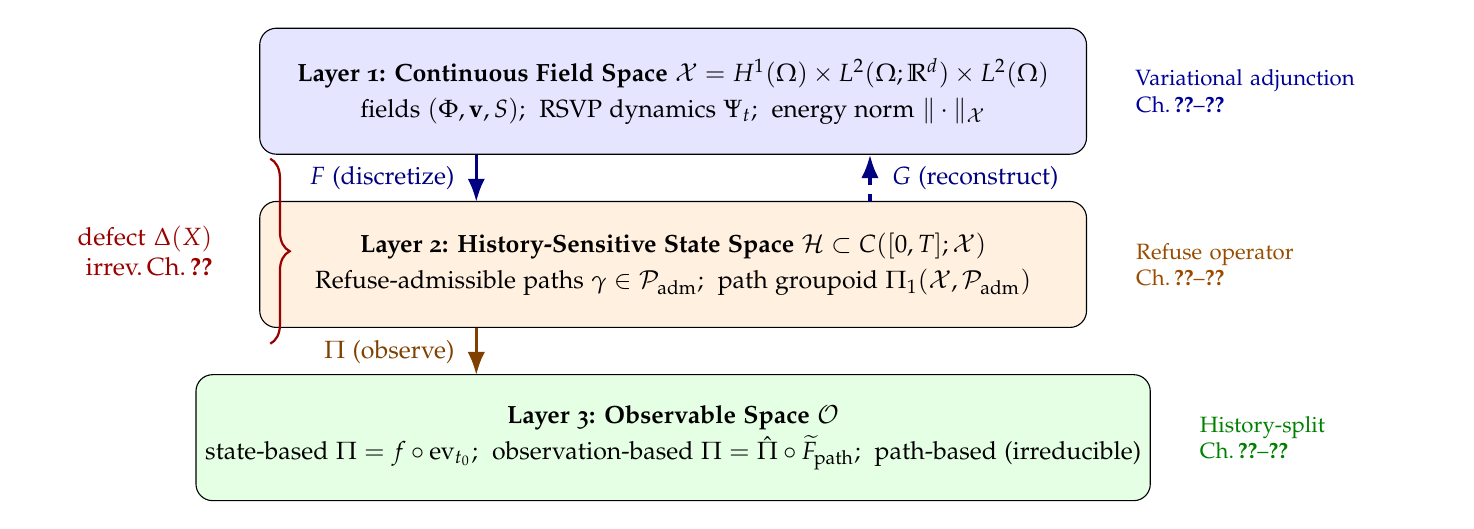
\begin{tikzpicture}[>=Latex, node distance=0pt]
  % Layer boxes
  \node[draw, rounded corners=6pt, fill=blue!10,
        minimum width=10.5cm, minimum height=1.6cm,
        font=\small\bfseries, align=center]
    (L1) at (0, 4.0)
    {Layer 1: Continuous Field Space $\X = H^1(\Omega)\times L^2(\Omega;\mathbb{R}^d)\times L^2(\Omega)$\\[2pt]
     \normalfont\small fields $(\Phi,\mathbf{v},S)$;\; RSVP dynamics $\Psi_t$;\; energy norm $\|\cdot\|_\X$};

  \node[draw, rounded corners=6pt, fill=orange!12,
        minimum width=10.5cm, minimum height=1.6cm,
        font=\small\bfseries, align=center]
    (L2) at (0, 1.8)
    {Layer 2: History-Sensitive State Space $\mathcal{H} \subset C([0,T];\X)$\\[2pt]
     \normalfont\small Refuse-admissible paths $\gamma\in\mathcal{P}_{\mathrm{adm}}$;\; path groupoid $\Pi_1(\X,\mathcal{P}_{\mathrm{adm}})$};

  \node[draw, rounded corners=6pt, fill=green!10,
        minimum width=10.5cm, minimum height=1.6cm,
        font=\small\bfseries, align=center]
    (L3) at (0,-0.4)
    {Layer 3: Observable Space $\mathcal{O}$\\[2pt]
     \normalfont\small state-based $\Pi = f\circ\mathrm{ev}_{t_0}$;\;
     observation-based $\Pi = \hat\Pi\circ\widetilde{F}_{\mathrm{path}}$;\;
     path-based (irreducible)};

  % Downward arrows with labels
  \draw[->, very thick, blue!50!black]
    (L1.south) ++(-2.5cm,0) -- ++(0,-0.6cm)
    node[midway, left=4pt, font=\small] {$F$ (discretize)};
  \draw[->, very thick, orange!50!black]
    (L2.south) ++(-2.5cm,0) -- ++(0,-0.6cm)
    node[midway, left=4pt, font=\small] {$\Pi$ (observe)};

  % Upward arrows with labels
  \draw[->, very thick, blue!50!black, dashed]
    (L1.south) ++(2.5cm,-0.6cm) -- ++(0,0.6cm)
    node[midway, right=4pt, font=\small] {$G$ (reconstruct)};

  % Right-side annotations
  \node[right=0.5cm of L1, font=\footnotesize, text=blue!60!black, align=left,
        text width=3.0cm]
    {Variational adjunction\\Ch.\,\ref{ch:adjunction}--\ref{ch:fixed-point}};
  \node[right=0.5cm of L2, font=\footnotesize, text=orange!60!black, align=left,
        text width=3.0cm]
    {Refuse operator\\Ch.\,\ref{ch:refuse}--\ref{ch:defect}};
  \node[right=0.5cm of L3, font=\footnotesize, text=green!50!black, align=left,
        text width=3.0cm]
    {History-split\\Ch.\,\ref{ch:history}--\ref{ch:split}};

  % Defect brace
  \draw[decorate,
        decoration={brace, amplitude=7pt, raise=4pt},
        thick, red!60!black]
    (L1.south west) ++(0,-0.05) -- ++(0,-2.35)
    node[midway, left=14pt, font=\small, red!60!black, align=right,
         text width=2.2cm]
    {defect $\Delta(X)$\\irrev.\,Ch.\,\ref{ch:irrev-dynamics}};
\end{tikzpicture}
\caption{The three-layer architecture of the RSVP adjunction framework.  Layer~1 (blue)
is the continuous configuration space with RSVP dynamics.  Layer~2 (orange) is the
history-sensitive path space with Refuse-admissible trajectories and the path groupoid
structure.  Layer~3 (green) is the observable space, where the central question is
whether the projection $\Pi$ requires full path data or factors through instantaneous
state.  The downward arrows $F$ and $\Pi$ project information; the upward dashed arrow
$G$ reconstructs it.  The red brace marks the defect produced by the non-invertibility
of $F$ — the structural source of irreversibility developed throughout Part~I.}
\label{fig:architecture}
\end{figure}

% ============================================================
\chapter{RSVP Field Dynamics}
\label{ch:rsvp}
% ============================================================

\section{The governing equations}

The RSVP system on $\Omega \times [0,T]$ is governed by three coupled
partial differential equations.  In the general form used throughout this monograph:

\begin{align}
  \partial_t \Phi &= \kappa_\Phi \Delta \Phi - \bv \cdot \nabla \Phi + f_\Phi(\Phi,\bv,S),
  \label{eq:phi}\\[4pt]
  \partial_t \bv &= \kappa_v \Delta \bv - c_0 \nabla S + f_v(\Phi,\bv,S),
  \label{eq:v}\\[4pt]
  \partial_t S &= \kappa_S \Delta S + \sigma_0(\Phi,\bv,S) + r(x,t).
  \label{eq:S}
\end{align}

Here $\Phi : \Omega \times [0,T] \to \mathbb{R}$ is the scalar coherence field,
$\bv : \Omega \times [0,T] \to \mathbb{R}^d$ is the vector transport field,
$S : \Omega \times [0,T] \to \mathbb{R}$ is the entropy field, and
$r : \Omega \times [0,T] \to \mathbb{R}$ is an externally specified entropy injection
rate representing contradiction input.  The coupling functions $f_\Phi$, $f_v$, and
$\sigma_0$ encode the interaction structure; the simplest nontrivial instance used in the
lattice computations of \cref{ch:split} takes
\begin{equation}
  \sigma_0 = -\nu S, \qquad f_v = c_0 \nabla S, \qquad f_\Phi = b\, \bv,
\end{equation}
with damping $\nu \in (0,1)$ and coupling constants $b, c_0 > 0$.

Natural boundary conditions are imposed: $\partial_n \Phi = \partial_n S = 0$ and
$\bv \cdot n = 0$ on $\partial\Omega$.

\begin{figure}[htbp]
\centering
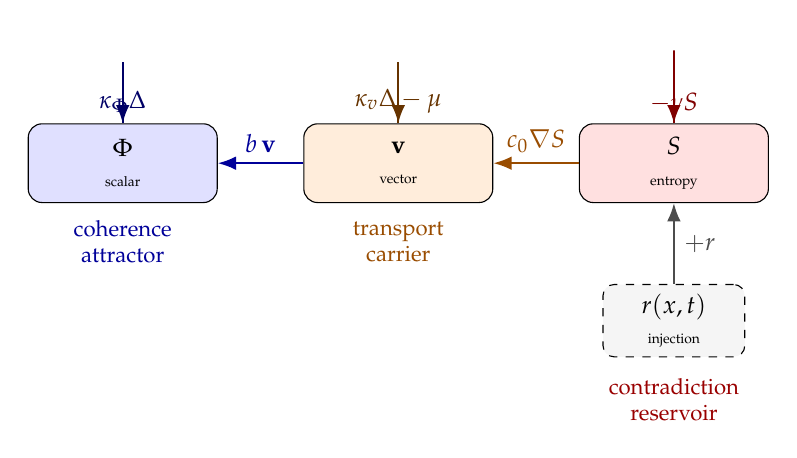
\begin{tikzpicture}[>=Latex, node distance=2.8cm]
  % Field nodes
  \node[draw, rounded corners=5pt, fill=blue!12,
        minimum width=2.4cm, minimum height=1.0cm,
        font=\bfseries\small, align=center]
    (Phi) at (-3.5, 0) {$\Phi$\\{\normalfont\tiny scalar}};

  \node[draw, rounded corners=5pt, fill=orange!14,
        minimum width=2.4cm, minimum height=1.0cm,
        font=\bfseries\small, align=center]
    (v) at (0, 0) {$\mathbf{v}$\\{\normalfont\tiny vector}};

  \node[draw, rounded corners=5pt, fill=red!12,
        minimum width=2.4cm, minimum height=1.0cm,
        font=\bfseries\small, align=center]
    (S) at (3.5, 0) {$S$\\{\normalfont\tiny entropy}};

  % External input
  \node[draw, dashed, rounded corners=4pt, fill=gray!8,
        minimum width=1.8cm, minimum height=0.8cm,
        font=\small, align=center]
    (r) at (3.5, -2.0) {$r(x,t)$\\{\tiny injection}};

  % Phi <-- v (b coupling)
  \draw[->, thick, blue!60!black]
    (v.west) -- (Phi.east)
    node[midway, above, font=\small] {$b\,\mathbf{v}$};

  % v <-- S (c_0 coupling)
  \draw[->, thick, orange!60!black]
    (S.west) -- (v.east)
    node[midway, above, font=\small] {$c_0\nabla S$};

  % S <-- r (injection)
  \draw[->, thick, gray!60!black]
    (r.north) -- (S.south)
    node[midway, right, font=\small] {$+r$};

  % S self-loop (damping)
  \draw[->, thick, red!50!black]
    (S.north) .. controls +(0,1.2) and +(0,1.2) .. (S.north)
    node[above, font=\small] {$-\nu S$};

  % Phi self-diffusion
  \draw[->, thick, blue!40!black]
    (Phi.north) .. controls +(0,1.0) and +(0,1.0) .. (Phi.north)
    node[above, font=\small] {$\kappa_\Phi\Delta$};

  % v self-damping
  \draw[->, thick, orange!40!black]
    (v.north) .. controls +(0,1.0) and +(0,1.0) .. (v.north)
    node[above, font=\small] {$\kappa_v\Delta - \mu$};

  % Mode labels below
  \node[blue!60!black, font=\footnotesize, align=center] at (-3.5,-1.0)
    {coherence\\attractor};
  \node[orange!60!black, font=\footnotesize, align=center] at (0,-1.0)
    {transport\\carrier};
  \node[red!60!black, font=\footnotesize, align=center] at (3.5, -3.0)
    {contradiction\\reservoir};
\end{tikzpicture}
\caption{RSVP field coupling structure.  The cascade flows right to left: entropy $S$
(red) drives the vector field $\mathbf{v}$ (orange) via the gradient coupling $c_0\nabla
S$, and the vector field drives the scalar $\Phi$ (blue) via the transport term $b\mathbf{v}$.
Each field has its own self-evolution (diffusion and damping, self-loops).  External
contradiction is injected through the entropy source $r(x,t)$.  This cascade structure
is the physical basis for the memory-depth table of \cref{ex:memory}: each active
coupling layer adds one time step to the minimal history-split horizon, because
information must propagate through the chain $r \to S \to \mathbf{v} \to \Phi$ before
exact cancellation is possible.}
\label{fig:rsvp-coupling}
\end{figure}

\section{Entropy production rate}

\begin{definition}[Entropy production rate density]
\label{def:sigma}
The local entropy production rate density is
\[
  \sigma(x,t) := \partial_t S(x,t) + \nabla \cdot \mathbf{j}_S(x,t),
\]
where $\mathbf{j}_S = -\kappa_S \nabla S$ is the entropy flux.  In the RSVP system,
\[
  \sigma(x,t) = \sigma_0(\Phi,\bv,S) + r(x,t) + \kappa_S \nnorm{\nabla S}^2 / S,
\]
with the last term arising from Fourier's law contributions when $S > 0$.  For the
linearized system used in the lattice, $\sigma(x,t) = r(x,t) - \nu S(x,t)$.
\end{definition}

\section{Discrete lattice reduction}

For the explicit constructions of \cref{ch:split,ch:bridge}, we reduce to a
one-dimensional $N$-site lattice with sites $i = 1, \dots, N$ and discrete time steps
$n = 0, 1, \dots, T$.  The update rules are:
\begin{align}
  \Phi_i(n+1) &= \Phi_i(n) + b\, v_i(n), \label{eq:lat-phi}\\
  v_i(n+1)   &= (1-\mu)\, v_i(n) + c\, \bigl(S_{i+1}(n) - S_{i-1}(n)\bigr),
  \label{eq:lat-v}\\
  S_i(n+1)   &= (1-\nu)\, S_i(n) + r_i(n), \label{eq:lat-S}
\end{align}
with reflecting boundary conditions $S_0 = S_1$, $S_{N+1} = S_N$.  Here
$\mu, \nu \in (0,1)$ are damping constants and $b, c > 0$ are coupling constants.
The center-channel reduced model used in \cref{ch:split} tracks only the antisymmetric
entropy-gradient variable $q(n) := S_{N}(n) - S_1(n)$ and the center-site values
$v(n) := v_{(N+1)/2}(n)$ and $\Phi(n) := \Phi_{(N+1)/2}(n)$, yielding
\begin{align}
  q(n+1)    &= \aq\, q(n) + 2u(n), \label{eq:red-q}\\
  v(n+1)    &= \av\, v(n) + c\, q(n), \label{eq:red-v}\\
  \Phi(n+1) &= \Phi(n) + b\, v(n), \label{eq:red-phi}
\end{align}
where $\aq := 1-\nu$, $\av := 1-\mu$, and $u(n)$ is the antisymmetric entropy injection
control at time $n$.

% ============================================================
\chapter{Discretization and the Refuse Operator}
\label{ch:refuse}
% ============================================================

\section{The Spherepop event operators}

The Spherepop calculus assigns to each trajectory a sequence of discrete events from the
alphabet $E := \{\mathsf{Pop}, \mathsf{Bind}, \mathsf{Collapse}, \mathsf{Refuse},
\mathsf{Null}\}$.  These operators act on the configuration space as follows.
$\mathsf{Pop}$ removes a resolved contradiction; $\mathsf{Bind}$ couples two coherence
regions; $\mathsf{Collapse}$ reduces a high-entropy zone to a lower-entropy attractor;
$\mathsf{Refuse}$ excludes a class of forward continuations; $\mathsf{Null}$ records no
event.

For the mathematical development, only $\mathsf{Refuse}$ plays a structural role; the
others may be treated as annotation operators that do not affect the trajectory-separation
argument.

\section{Refuse as a constraint on forward extensions}

\begin{definition}[Forward extension set]
For any path $\gamma \in \PP$ and time $t_0 \in [0,T)$, the \emph{forward extension set}
is
\[
  \mathrm{Ext}(\gamma, t_0) :=
  \bigl\{ \tilde\gamma \in \PP : \tilde\gamma|_{[0,t_0]} = \gamma|_{[0,t_0]} \bigr\}.
\]
\end{definition}

\begin{definition}[Refuse event]
\label{def:refuse}
A \emph{Refuse event} at time $t_0$ along a path $\gamma$ is the specification of a
proper closed subset
\[
  \mathcal{C}(\gamma, t_0) \subsetneq \mathrm{Ext}(\gamma, t_0)
\]
satisfying:
\begin{enumerate}
  \item\label{it:ref-nontrivial}
        (Nontrivial exclusion) $\mathcal{C}(\gamma,t_0) \ne \mathrm{Ext}(\gamma,t_0)$.
  \item\label{it:ref-closed}
        (Closedness) $\mathcal{C}(\gamma,t_0)$ is closed in the path topology.
  \item\label{it:ref-consistent}
        (Forward consistency) If $\tilde\gamma \in \mathcal{C}(\gamma,t_0)$, then any
        restriction of $\tilde\gamma$ to $[t_0, t_1]$, $t_1 < T$, is admissible.
\end{enumerate}
A path is \emph{Refuse-admissible} if at each Refuse event time $t_0 \in
\mathcal{T}_{\mathrm{Refuse}}(\gamma)$, its actual continuation lies in
$\mathcal{C}(\gamma, t_0)$.
\end{definition}

\section{Refuse-separated pairs}

\begin{definition}[Refuse-separated pair]
\label{def:refuse-sep}
Two paths $\gamma_1, \gamma_2 \in \PP$ are \emph{Refuse-separated at time $t_0$} if:
\begin{enumerate}
  \item $\gamma_1|_{[0,t_0]} = \gamma_2|_{[0,t_0]}$ (agreement up to $t_0$);
  \item $\gamma_1 \in \mathcal{C}(\gamma_1, t_0)$ and
        $\gamma_2 \notin \mathcal{C}(\gamma_1, t_0)$ (exactly one is admitted).
\end{enumerate}
\end{definition}

Refuse-separation captures the essential feature that the system reaches the same
instantaneous configuration but one forward continuation is forbidden.  This is precisely
where state-based description fails: the two paths are observationally equivalent at
$t_0$ yet dynamically inequivalent thereafter.

\begin{figure}[htbp]
\centering
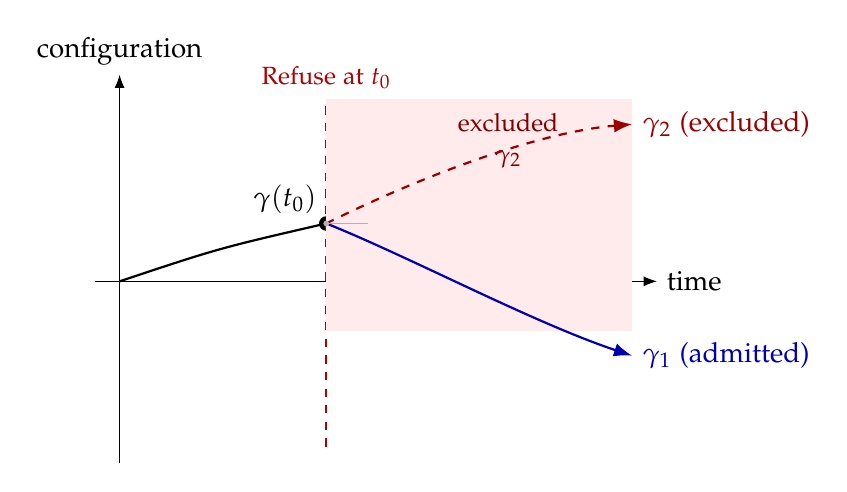
\begin{tikzpicture}[>=Latex, scale=1.05]
  % Configuration space axis (horizontal = time, vertical = configuration)
  \draw[->] (-0.3, 0) -- (6.5, 0) node[right] {time};
  \draw[->] (0, -2.2) -- (0, 2.5) node[above] {configuration};

  % Shared past: single trajectory up to t_0
  \draw[thick, black] (0, 0) .. controls (1.2, 0.4) .. (2.5, 0.7);
  \fill (2.5, 0.7) circle (2.5pt) node[above left] {$\gamma(t_0)$};

  % Refuse boundary at t_0
  \draw[dashed, red!70!black, thick] (2.5, -2.0) -- (2.5, 2.2)
    node[above, font=\small, red!70!black] {Refuse at $t_0$};
  % Excluded zone shading
  \fill[red!8] (2.5, -0.6) rectangle (6.2, 2.2);
  \node[red!50!black, font=\small, align=center] at (4.7, 1.7)
    {excluded\\$\gamma_2$};

  % Admitted branch gamma_1
  \draw[->, thick, blue!70!black]
    (2.5, 0.7) .. controls (3.5, 0.3) and (5.0, -0.5) .. (6.2, -0.9)
    node[right, blue!70!black] {$\gamma_1$ (admitted)};

  % Excluded branch gamma_2 (dashed, in red zone)
  \draw[->, dashed, thick, red!60!black]
    (2.5, 0.7) .. controls (3.5, 1.2) and (5.0, 1.8) .. (6.2, 1.9)
    node[right, red!60!black] {$\gamma_2$ (excluded)};

  % Saddle-like crossing lines to show bifurcation character
  \draw[thin, gray!60] (2.5, 0.7) -- (3.0, 0.7);
  \fill[gray!60] (2.5, 0.7) circle (1pt);
\end{tikzpicture}
\caption{Trajectory bifurcation induced by a Refuse event at time $t_0$.  Both branches
agree on $[0, t_0]$ and arrive at the same instantaneous configuration $\gamma(t_0)$,
but $\gamma_2$ is excluded by the Refuse constraint $\mathcal{C}(\gamma, t_0)$
(shaded region).  Only $\gamma_1$ is Refuse-admissible.  This is the discrete-time
analog of a saddle point where the forward dynamics bifurcate irreversibly.}
\label{fig:refuse-bifurcation}
\end{figure}

\section{The surrogate discretization map}

The actual discretization $F_{\mathrm{true}}: \X \to \Hcal$ involves symbolic event
assignment and thresholding operations that may not be weakly continuous.  To secure
the existence arguments of \cref{ch:adjunction}, we first work with a continuous
surrogate.

\begin{definition}[Surrogate discretization]
\label{def:Ftilde}
Choose test functions $\{\psi_j\}_{j=1}^m \subset H^1(\Omega)$,
$\{\chi_j\}_{j=1}^m \subset L^2(\Omega;\mathbb{R}^d)$,
$\{\eta_j\}_{j=1}^m \subset L^2(\Omega)$.  Define
\[
  \Ft : \X \to \mathcal{Y} := \mathbb{R}^{3m}, \qquad
  \Ft(X) := \bigl(
    \ip{\Phi}{\psi_j},\, \ip{\bv}{\chi_j},\, \ip{S}{\eta_j}
  \bigr)_{j=1}^m.
\]
This map is bounded linear, hence weakly continuous.
\end{definition}

The surrogate encodes finitely many moments of the field triple.  It is related to the
true discretization by a composition $F_{\mathrm{true}} = Q \circ \Ft$, where
$Q: \mathcal{Y} \to \Hcal$ is a symbolic quantization map.  The foundation of the adjunction
rests on $\Ft$; the symbolic layer is layered on afterward in \cref{ch:defect}.

% ============================================================
\chapter{The Variational Adjunction and Irreversibility}
\label{ch:adjunction}
% ============================================================

\section{The reconstruction functional}

\begin{definition}[Reconstruction functional]
\label{def:L}
For $y = (y_\Phi, y_v, y_S) \in \mathcal{Y}$, define
\begin{equation}\label{eq:L}
  L(X \mid y) :=
  \frac{\kappa}{2}\nnorm{\nabla\Phi}_{L^2}^2
  + \frac{\alpha}{2}\nnorm{\Phi}_{L^2}^2
  + \frac{\lambda}{2}\nnorm{\bv}_{L^2}^2
  + \frac{\beta}{2}\nnorm{S}_{L^2}^2
  + \frac{\gamma}{2}\nnorm{\Ft(X) - y}_{\mathcal{Y}}^2,
\end{equation}
with constants $\kappa, \alpha, \lambda, \beta, \gamma > 0$.
\end{definition}

\begin{remark}
The quadratic regularization in $S$ (the term $\frac{\beta}{2}\nnorm{S}_{L^2}^2$) is
necessary; a linear term $\beta \int_\Omega S\, dx$ is not coercive on $L^2(\Omega)$.
This correction was identified during the construction of Note~I.
\end{remark}

\begin{figure}[htbp]
\centering
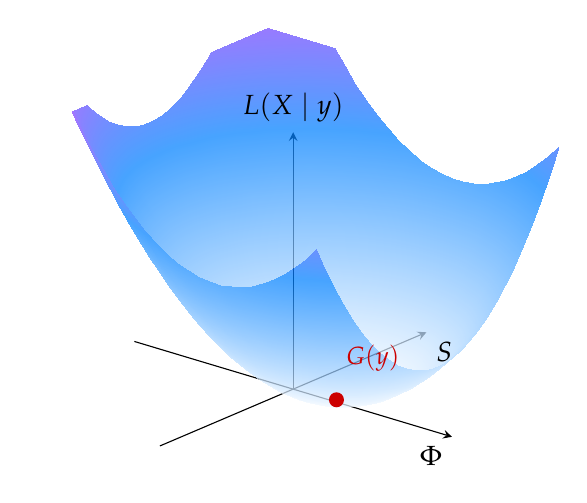
\begin{tikzpicture}
\begin{axis}[
  view = {40}{30},
  axis lines = center,
  xlabel = {$\Phi$}, ylabel = {$S$}, zlabel = {$L(X \mid y)$},
  xlabel style = {anchor=north east},
  ylabel style = {anchor=north west},
  zlabel style = {anchor=south},
  xmin = -2.2, xmax = 2.2,
  ymin = -2.2, ymax = 2.2,
  zmin = 0,   zmax = 5.5,
  xtick = \empty, ytick = \empty, ztick = \empty,
  width = 9cm, height = 7.5cm,
  colormap/cool,
  samples = 28,
  domain = -2:2
]
  % Surface: L(Phi, S | y) = (Phi-0.6)^2 + S^2 (schematic 2D slice)
  \addplot3[
    surf,
    opacity = 0.72,
    shader = interp,
    domain = -2:2,
    y domain = -2:2
  ] { 0.7*(x-0.6)^2 + 0.9*y^2 + 0.05 };
  % Minimum point G(y)
  \addplot3[
    only marks,
    mark = *,
    mark size = 2.5pt,
    color = red!80!black
  ] coordinates { (0.6, 0, 0.05) };
  % Label minimum
  \node[red!80!black, font=\small] at (axis cs: 0.6, 0.6, 0.6) {$G(y)$};
\end{axis}
\end{tikzpicture}
\caption{Schematic energy landscape of the reconstruction functional $L(X \mid y)$
as a function of the scalar and entropy field components, with the feature target
$y$ fixed.  The unique global minimum (red dot) is the reconstruction $G(y)$,
the canonical representative selected from the fiber $\Ft^{-1}(y)$.  The bowl
shape reflects the strict convexity established in \cref{thm:existence}.}
\label{fig:energy-landscape}
\end{figure}

\section{Existence and uniqueness of minimizers}

\begin{theorem}[Existence and uniqueness of reconstruction]
\label{thm:existence}
For every $y \in \mathcal{Y}$, the functional $L(\cdot \mid y)$ admits a unique minimizer
$X^\sharp = G(y) \in \X$.
\end{theorem}

\begin{proof}
Let $(X_n) \subset \X$ be a minimizing sequence: $L(X_n \mid y) \to \inf_{X \in \X}
L(X \mid y)$.  Since all coefficients are positive,
\[
  L(X_n \mid y) \ge
  \frac{\kappa}{2}\nnorm{\nabla\Phi_n}_{L^2}^2
  + \frac{\alpha}{2}\nnorm{\Phi_n}_{L^2}^2
  + \frac{\lambda}{2}\nnorm{\bv_n}_{L^2}^2
  + \frac{\beta}{2}\nnorm{S_n}_{L^2}^2
  \ge c\, \nnorm{X_n}_\X^2
\]
for $c = \min\{\kappa,\alpha,\lambda,\beta\}/2 > 0$.  Hence $(X_n)$ is bounded in the
Hilbert space $\X$, so there exists a subsequence (not relabeled) with
$X_n \rightharpoonup X_* \in \X$.

Each quadratic norm term is weakly lower semicontinuous.  Since $\Ft$ is bounded linear,
it is weakly continuous; thus $\Ft(X_n) \to \Ft(X_*)$ strongly in $\mathcal{Y}$
(finite-dimensional), and
$\nnorm{\Ft(X_*) - y}^2 = \lim_n \nnorm{\Ft(X_n) - y}^2$.  Therefore
\[
  L(X_* \mid y) \le \liminf_n L(X_n \mid y),
\]
and $X_*$ is a minimizer.

Uniqueness follows from strict convexity: the terms $\frac{\kappa}{2}\nnorm{\nabla\Phi}^2
+ \frac{\alpha}{2}\nnorm{\Phi}^2$ are strictly convex in $\Phi$, and similarly for
$\bv$ and $S$, so the whole functional is strictly convex on $\X$.
\end{proof}

\section{The reconstruction operator and its Euler--Lagrange system}

\begin{definition}[Reconstruction operator]
\label{def:G}
Define $G: \mathcal{Y} \to \X$ by $G(y) := \argmin_{X \in \X} L(X \mid y)$.
\end{definition}

Because $L$ is block-diagonal in the three components, the minimizer satisfies a
decoupled elliptic system.  Writing $F_\Phi, F_v, F_S$ for the three blocks of $\Ft$
and $F_\Phi^*, F_v^*, F_S^*$ for their $L^2$-adjoints:

\begin{align}
  (-\kappa\Delta + \alpha I + \gamma F_\Phi^* F_\Phi)\,\Phi^\sharp
    &= \gamma F_\Phi^* y_\Phi, \label{eq:EL-phi}\\
  (\lambda I + \gamma F_v^* F_v)\,\bv^\sharp
    &= \gamma F_v^* y_v, \label{eq:EL-v}\\
  (\beta I + \gamma F_S^* F_S)\, S^\sharp
    &= \gamma F_S^* y_S. \label{eq:EL-S}
\end{align}

Since the test functions are finite in number, $F_\Phi^* F_\Phi$ is a finite-rank
self-adjoint operator, and the operator on the left of \cref{eq:EL-phi} is strictly
coercive on $H^1(\Omega)$.  Hence $G$ is well-defined as a linear operator:
\begin{equation}
  G = A^{-1} b(\cdot),
\end{equation}
where $A$ is the block operator assembled from the left-hand sides of
\crefrange{eq:EL-phi}{eq:EL-S} and $b(y)$ assembles the right-hand sides.

\section{Stability of the reconstruction operator}

\begin{theorem}[Lipschitz stability]
\label{thm:lipschitz}
The reconstruction operator $G: \mathcal{Y} \to \X$ is globally Lipschitz:
\[
  \nnorm{G(y) - G(z)}_\X \le C_G\, \nnorm{y - z}_{\mathcal{Y}}
\]
for an explicit constant $C_G := \max\{C_\Phi, C_v, C_S\}$, where
\[
  C_\Phi = \frac{\gamma \nnorm{F_\Phi}}{\min\{\kappa,\alpha\}}, \qquad
  C_v   = \frac{\gamma \nnorm{F_v}}{\lambda}, \qquad
  C_S   = \frac{\gamma \nnorm{F_S}}{\beta}.
\]
\end{theorem}

\begin{proof}
For the $\Phi$-component: let $u = \Phi^\sharp(y) - \Phi^\sharp(z)$.  The difference
satisfies $(-\kappa\Delta + \alpha I + \gamma F_\Phi^*F_\Phi)u = \gamma F_\Phi^*(y_\Phi
- z_\Phi)$.  Testing against $u$ and applying the coercivity bound
$\kappa\nnorm{\nabla u}^2 + \alpha\nnorm{u}^2 \ge \min\{\kappa,\alpha\}\nnorm{u}_{H^1}^2$
together with Cauchy--Schwarz and boundedness of $F_\Phi$ gives $C_\Phi$ as stated.  The
arguments for $\bv$ and $S$ are analogous ($L^2$-level, no gradient term).  Assembling
the three estimates with the Euclidean norm on $\mathcal{Y}$ yields the global Lipschitz
constant.
\end{proof}

\section{The comparison map and irreversibility}

\begin{definition}[Comparison map and reconstruction defect]
\label{def:eta}
Define the comparison map $\eta: \X \to \X$ by
\[
  \eta := G \circ \Ft.
\]
The \emph{reconstruction defect} of $X \in \X$ is
\[
  \Delta(X) := \nnorm{X - \eta(X)}_\X.
\]
\end{definition}

By composition of Lipschitz maps, $\eta$ is globally Lipschitz with constant
$C_\eta \le C_G \nnorm{\Ft}$.  Hence $\Delta$ is globally Lipschitz:
$|\Delta(X) - \Delta(X')| \le (1 + C_\eta)\nnorm{X - X'}_\X$.

\begin{figure}[htbp]
\centering
\begin{tikzcd}[column sep=3.5em, row sep=3em, ampersand replacement=\&]
  \X \arrow[r, "\Ft"]
     \arrow[dr, "\eta = G \circ \Ft"', bend right=15]
  \& \mathcal{Y} \arrow[d, "G"] \\
  \& \X
\end{tikzcd}
\qquad\qquad
\begin{tikzcd}[column sep=3.0em, ampersand replacement=\&]
  \X \arrow[r, "\Ft"]
     \arrow[rr, bend left=30, "\mathrm{id}_\X"']
  \& \mathcal{Y} \arrow[r, "G"]
  \& \X
\end{tikzcd}
\caption{\textbf{Left:} Adjunction structure $\widetilde{F} \dashv G$ with unit
$\eta = G \circ \widetilde{F}$.  \textbf{Right:} The triangle $G \circ \widetilde{F}
\neq \mathrm{id}_\X$ fails generically; this failure is the categorical formulation of
irreversibility.  When $\widetilde{F}$ is non-injective, no right inverse $G$ can
make the outer triangle commute for all $X \in \X$.}
\label{fig:adjunction}
\end{figure}

\begin{theorem}[Irreversibility as non-identity of reconstruction]
\label{thm:irrev}
If $\Ft$ is not injective, then $\eta$ is not the identity, and there exist configurations
$X \in \X$ with $\Delta(X) > 0$.
\end{theorem}

\begin{proof}
Suppose $\Ft(X_1) = \Ft(X_2) = y$ for distinct $X_1, X_2 \in \X$.  Then
$\eta(X_1) = G(y) = \eta(X_2)$.  If $X_1 \ne G(y)$, then $\Delta(X_1) > 0$.  If
$X_1 = G(y)$, then $X_2 = G(y) = X_1$, contradicting distinctness.  Therefore at least
one of $X_1, X_2$ has positive defect.
\end{proof}

\begin{remark}
Irreversibility is not the mere existence of a non-injective map; many maps fail
injectivity in ways that carry no thermodynamic content.  The content here is that $G$ is
the \emph{optimal} reconstruction---the unique minimizer of $L(\cdot \mid y)$---and the
loss is what remains after the best possible recovery.  Loss is therefore not assumed;
it is the universal defect of reconstruction.
\end{remark}

% ============================================================
\chapter{Refuse-Admissible Measurable Structure and Entropy Defect}
\label{ch:defect}
% ============================================================

\section{The admissible $\sigma$-algebra}

\begin{definition}[Refuse-admissible $\sigma$-algebra]
\label{def:sigma-alg}
The \emph{Refuse-admissible $\sigma$-algebra} on $\X$ is
\[
  \Aadm := \sigma\bigl(\{X \in \X : X = \gamma(t)
    \text{ for some } \gamma \in \Padm,\, t \in [0,T]\}\bigr).
\]
This is the $\sigma$-algebra generated by all configurations reachable by a
Refuse-admissible path.
\end{definition}

We have $\Aadm \subseteq \mathcal{B}(\X)$ (Borel $\sigma$-algebra on $\X$).  When the
excluded set $\mathcal{E} = \emptyset$ and Refuse imposes no constraint, $\Aadm =
\mathcal{B}(\X)$.  Nontrivial Refuse constraints make $\Aadm$ strictly smaller.

\begin{assumption}[Admissibility of reference measure]
\label{ass:mu}
The reference measure $\mu$ on $(\X, \mathcal{B}(\X))$ satisfies $\mu(\X \setminus
\Aadm) = 0$; equivalently, $\mu$ is a measure on $(\X, \Aadm)$.
\end{assumption}

\section{Refuse observability}

The bridge from the categorical Refuse operator to the measurable defect requires that
Refuse-induced trajectory distinctions survive projection through $\Ft$.

\begin{assumption}[Refuse observability]
\label{ass:obs}
For any Refuse-separated pair $(\gamma_1, \gamma_2)$ (in the sense of
\cref{def:refuse-sep}), we have
\[
  \Fpath(\gamma_1) \ne \Fpath(\gamma_2),
\]
where $\Fpath(\gamma) := (\Ft(\gamma(t)))_{t \in [0,T]} \in C([0,T];\mathcal{Y})$.
\end{assumption}

\begin{theorem}[Injectivity on Refuse-admissible trajectory classes]
\label{thm:injectivity}
Under \cref{ass:obs}, the path-level map $\Fpath: \Padm \to C([0,T];\mathcal{Y})$
is injective on Refuse-separated trajectory pairs.
\end{theorem}

\begin{proof}
Immediate from \cref{def:refuse-sep,ass:obs}: distinct Refuse-separated trajectories
map to distinct feature paths.
\end{proof}

\section{The entropy defect via Jensen--Shannon divergence}

Since $G$ is globally Lipschitz (\cref{thm:lipschitz}), the comparison map $\eta = G
\circ \Ft$ is Borel measurable.  The reconstructed measure is well-defined:

\begin{definition}[Reconstructed measure and entropy defect]
\label{def:defect-meas}
Let $\mu$ satisfy \cref{ass:mu}.  Define the reconstructed measure
$\tilde\mu := \eta_* \mu$ (the pushforward of $\mu$ through $\eta$).  The
\emph{entropy defect} is
\begin{equation}\label{eq:Djs}
  \mathcal{D}(\Ft, G, \mu) := \Djs(\mu, \tilde\mu) :=
  \tfrac{1}{2}\KL\!\bigl(\mu \,\Vert\, \tfrac{\mu+\tilde\mu}{2}\bigr)
  + \tfrac{1}{2}\KL\!\bigl(\tilde\mu \,\Vert\, \tfrac{\mu+\tilde\mu}{2}\bigr).
\end{equation}
\end{definition}

\begin{remark}
The Jensen--Shannon divergence replaces the raw KL divergence $\KL(\mu \| \tilde\mu)$
because $\tilde\mu$ may fail to be absolutely continuous with respect to $\mu$ when
$\eta$ collapses distinct configurations onto a canonical representative.  That collapse
is itself the measure-theoretic signature of projection loss.  $\Djs$ is always
finite, bounded in $[0, \log 2]$, symmetric, and vanishes if and only if $\tilde\mu =
\mu$.
\end{remark}

\begin{proposition}[Defect positivity on Refuse strata]
\label{prop:defect-pos}
Under \cref{ass:mu,ass:obs}, if $A \subset \X$ is a set of positive $\mu$-measure
consisting of configurations lying on trajectories that differ by a Refuse event, then
$\Delta(X) > 0$ for all $X \in A$, and consequently $\mathcal{D}(\Ft, G, \mu) > 0$.
\end{proposition}

\begin{proof}
By \cref{thm:injectivity}, configurations on Refuse-separated trajectories are
distinguished by $\Fpath$; hence they are distinguished by their feature encodings
$\Ft(\gamma(t))$.  By uniqueness of the minimizer (\cref{thm:existence}), distinct
feature encodings yield distinct canonical reconstructions.  Therefore $X \ne \eta(X)$
for $X \in A$, giving $\Delta(X) > 0$ on $A$.  Since $\mu(A) > 0$, the supports of
$\mu$ and $\tilde\mu$ differ on $A$, so $\Djs(\mu, \tilde\mu) > 0$.
\end{proof}

\begin{proposition}[Monotonicity under coarsening]
\label{prop:monotone}
Let $\Ft_1$ and $\Ft_2$ be two feature maps with $\Ft_2 = A \circ \Ft_1$ for some
bounded linear $A$ with $\nnorm{A} \le 1$, and let $G_1, G_2$ be the corresponding
reconstruction operators.  Then
$\mathcal{D}(\Ft_2, G_2, \mu) \le \mathcal{D}(\Ft_1, G_1, \mu)$.
\end{proposition}

\begin{proof}
A coarser discretization loses at least as much information.  The data-processing
inequality for Jensen--Shannon divergence \cite{lin1991} gives the result.
\end{proof}

% ============================================================
\chapter{Functional-Analytic Foundations of the Configuration Space}
\label{ch:fa-foundations}
% ============================================================

\section{The underlying domain}

Let $\Omega \subset \mathbb{R}^d$ be a bounded open domain with Lipschitz boundary.
All fields are defined on $\Omega$ and all integrals are taken with respect to Lebesgue
measure unless otherwise specified.  The Lipschitz boundary condition ensures the
validity of the Sobolev trace and extension theorems, the Rellich--Kondrachov compact
embedding $H^1(\Omega) \hookrightarrow L^2(\Omega)$, and the Poincaré--Wirtinger
inequality.

\section{Sobolev structure of the field components}

The three RSVP fields are assigned to Sobolev spaces according to the regularity required
by the governing PDEs and the reconstruction functional:
\begin{itemize}
  \item The scalar coherence field: $\Phi \in H^1(\Omega)$, with norm
        $\nnorm{\Phi}_{H^1}^2 := \nnorm{\Phi}_{L^2}^2 + \nnorm{\nabla\Phi}_{L^2}^2$;
  \item The vector transport field: $\bv \in L^2(\Omega;\mathbb{R}^d)$;
  \item The entropy field: $S \in L^2(\Omega)$.
\end{itemize}
The choice of $H^1$ for $\Phi$ is necessitated by the gradient term $\frac{\kappa}{2}
\nnorm{\nabla\Phi}_{L^2}^2$ in the reconstruction functional; $L^2$ regularity alone
would not give coercive control over $\nabla\Phi$.  The $L^2$ choice for $\bv$ and $S$
is the minimal space in which the quadratic regularization terms are finite.

\section{Completeness and separability of $\X$}

\begin{proposition}[Hilbert space structure of $\X$]
\label{prop:X-hilbert}
The configuration space $\X = H^1(\Omega) \times L^2(\Omega;\mathbb{R}^d) \times
L^2(\Omega)$ with inner product
\[
  \ip{X}{Y}_\X := \ip{\Phi_X}{\Phi_Y}_{H^1} + \ip{\bv_X}{\bv_Y}_{L^2}
                  + \ip{S_X}{S_Y}_{L^2}
\]
is a separable Hilbert space.
\end{proposition}

\begin{proof}
Each component space is a separable Hilbert space: $H^1(\Omega)$ is separable since
$\Omega \subset \mathbb{R}^d$ is a bounded Lipschitz domain (the eigenfunctions of the
Neumann Laplacian form a countable orthonormal basis); $L^2(\Omega;\mathbb{R}^d)$ and
$L^2(\Omega)$ are separable by standard measure theory.  The product of finitely many
separable Hilbert spaces is again a separable Hilbert space.  Completeness of each factor
and the product norm are standard.
\end{proof}

\section{Admissible energy subspace}

\begin{definition}[Admissible energy subspace]
\label{def:XM}
For $M > 0$, define
\[
  \X_M := \{X \in \X : \nnorm{X}_\X \le M\}.
\]
\end{definition}

\begin{proposition}[Compactness of $\X_M$]
\label{prop:XM-compact}
The set $\X_M$ is closed, convex, and weakly sequentially compact in $\X$.  Moreover,
the $\Phi$-component of any bounded sequence in $\X_M$ admits a subsequence converging
strongly in $L^2(\Omega)$ (Rellich--Kondrachov).
\end{proposition}

\begin{proof}
Closedness and convexity of $\X_M$ are immediate from the properties of the norm.  Weak
sequential compactness follows from the reflexivity of Hilbert spaces (Banach--Alaoglu
theorem).  For the strong $L^2$-compactness of the $\Phi$-component: any bounded
sequence in $H^1(\Omega)$ is precompact in $L^2(\Omega)$ by the Rellich--Kondrachov
theorem, which applies since $\Omega$ is a bounded Lipschitz domain.
\end{proof}

\section{Weak lower semicontinuity and the direct method}

The key analytical property for variational arguments is weak lower semicontinuity of
the relevant functionals.

\begin{proposition}[Weak lower semicontinuity of $L(\cdot \mid y)$]
\label{prop:wlsc}
For each $y \in \mathcal{Y}$, the reconstruction functional $L(\cdot \mid y)$ is weakly
lower semicontinuous on $\X$.
\end{proposition}

\begin{proof}
The squared norm terms $\nnorm{\nabla\Phi}_{L^2}^2$, $\nnorm{\bv}_{L^2}^2$,
$\nnorm{S}_{L^2}^2$ are weakly lower semicontinuous as squared norms on Hilbert spaces.
The quadratic term $\nnorm{\Ft(X) - y}_{\mathcal{Y}}^2$ is continuous (hence weakly
continuous) since $\Ft$ is bounded linear and the norm on the finite-dimensional space
$\mathcal{Y}$ is continuous.  The sum of weakly lower semicontinuous functions is weakly
lower semicontinuous.
\end{proof}

Together with coercivity (established in \cref{ch:adjunction}), \cref{prop:wlsc} and
\cref{prop:XM-compact} complete the verification of the direct method's hypotheses for
the reconstruction problem: every minimizing sequence is bounded (by coercivity), admits
a weakly convergent subsequence (by compactness), and the functional evaluates favorably
at the limit (by weak lower semicontinuity).

% ============================================================
\chapter{Well-Posedness of the RSVP Dynamics}
\label{ch:wellposed}
% ============================================================

\section{Abstract formulation of the coupled system}

The RSVP system \crefrange{eq:phi}{eq:S} can be written in abstract form as
\[
  \frac{dX}{dt} = \mathcal{A}X + \mathcal{N}(X), \qquad X(0) = X_0 \in \X,
\]
where $\mathcal{A}: D(\mathcal{A}) \subset \X \to \X$ is the principal part operator and
$\mathcal{N}: \X \to \X$ encodes the coupling nonlinearities and the entropy source term.
The linear part is given by
\[
  \mathcal{A}
  \begin{pmatrix} \Phi \\ \bv \\ S \end{pmatrix}
  :=
  \begin{pmatrix}
    \kappa_\Phi \Delta \Phi \\
    \kappa_v \Delta \bv - c_0 \nabla S \\
    \kappa_S \Delta S - \nu S
  \end{pmatrix},
\]
with domain $D(\mathcal{A}) = (H^2(\Omega) \cap H^1_N(\Omega)) \times H^1(\Omega;\mathbb{R}^d)
\times H^1(\Omega)$, where $H^1_N$ denotes functions satisfying Neumann boundary
conditions.

\section{Semigroup generation}

\begin{proposition}[Generation of $C^0$-semigroup]
\label{prop:semigroup}
The operator $\mathcal{A}$ with domain $D(\mathcal{A})$ generates a $C^0$-semigroup
$(e^{t\mathcal{A}})_{t \ge 0}$ on $\X$.
\end{proposition}

\begin{proof}
The Neumann Laplacian $-\Delta$ on $L^2(\Omega)$ with domain $H^2(\Omega) \cap
H^1_N(\Omega)$ is a non-negative self-adjoint operator and generates an analytic
semigroup on $L^2(\Omega)$ \cite{evans2010}.  The diffusion operator $\kappa_S(\Delta -
\nu I/\kappa_S)$ on the entropy component is therefore analytic with shift.  The
coupling terms $-c_0\nabla S$ and $c_0\nabla\cdot\bv$ are bounded perturbations of the
diagonal semigroup generator (they map $H^1$ into $L^2$), so by standard perturbation
theory for $C^0$-semigroups \cite{pazy1983}, $\mathcal{A}$ generates a $C^0$-semigroup
on $\X$.
\end{proof}

\section{Assumptions on the nonlinear term}

\begin{assumption}[Nonlinear growth and Lipschitz conditions]
\label{ass:nonlinear}
The map $\mathcal{N}: \X \to \X$ satisfies:
\begin{enumerate}
  \item (Local Lipschitz) For every $R > 0$ there exists $L_R > 0$ such that
        $\nnorm{\mathcal{N}(X) - \mathcal{N}(Y)}_\X \le L_R \nnorm{X-Y}_\X$
        for all $X, Y \in \X_R$;
  \item (At most linear growth) $\nnorm{\mathcal{N}(X)}_\X \le C(1 + \nnorm{X}_\X)$
        for all $X \in \X$.
\end{enumerate}
\end{assumption}

The simplest nonlinear coupling terms in RSVP (e.g., $\rho S \Phi^2$ projected into
$L^2$) satisfy \cref{ass:nonlinear} by Sobolev multiplication theorems on bounded
domains \cite{evans2010}.

\section{Existence, uniqueness, and continuous dependence}

\begin{theorem}[Global well-posedness of RSVP]
\label{thm:wellposed}
Under \cref{ass:nonlinear}, for every $X_0 \in \X$, the abstract RSVP system admits a
unique mild solution $X \in C([0,\infty); \X)$ satisfying
\[
  X(t) = e^{t\mathcal{A}} X_0 + \int_0^t e^{(t-s)\mathcal{A}} \mathcal{N}(X(s))\, ds.
\]
Moreover, solutions depend continuously on initial data: if $X_1(0), X_2(0) \in \X$
then
\[
  \nnorm{X_1(t) - X_2(t)}_\X \le C_T \nnorm{X_1(0) - X_2(0)}_\X
  \quad \text{for } t \in [0,T].
\]
\end{theorem}

\begin{proof}
Local existence and uniqueness follow from the contraction mapping principle applied to
the integral equation on $C([0,\tau]; \X)$ for small $\tau > 0$, using the local Lipschitz
condition of \cref{ass:nonlinear}.  Global existence follows from the linear growth
condition and a Grönwall argument: defining $E(t) = \nnorm{X(t)}_\X^2$, the energy
inequality gives $E(t) \le E(0) e^{Ct} + C'$, preventing finite-time blow-up.
Continuous dependence on initial data is obtained by applying Grönwall's inequality
to the difference $X_1(t) - X_2(t)$.
\end{proof}

\section{The solution operator}

\begin{definition}[Solution operator]
\label{def:Psi}
For each $t \ge 0$, define the \emph{solution operator}
\[
  \Psi_t: \X \to \X, \qquad \Psi_t(X_0) := X(t),
\]
where $X(t)$ is the unique mild solution of the RSVP system with initial condition $X_0$.
\end{definition}

\begin{proposition}[Semigroup properties of $\Psi_t$]
\label{prop:Psi-semigroup}
The family $(\Psi_t)_{t \ge 0}$ satisfies:
\begin{enumerate}
  \item $\Psi_0 = \mathrm{id}_\X$;
  \item $\Psi_{t+s} = \Psi_t \circ \Psi_s$ for all $t, s \ge 0$;
  \item $t \mapsto \Psi_t(X_0)$ is continuous for each $X_0 \in \X$.
\end{enumerate}
\end{proposition}

The solution operator $\Psi_t$ is the object that turns the path space $\PP$ into a
legitimate mathematical domain for the admissible trajectory analysis of \cref{ch:refuse}.
Specifically, every admissible path $\gamma \in \Padm$ is of the form $\gamma(t) =
\Psi_t(X_0)$ for some initial condition $X_0$ and some admissible source term; the
Refuse operator then acts on the future extensions of such orbits.

% ============================================================
\chapter{The Discretization Map and Induced Quotient Structure}
\label{ch:quotient}
% ============================================================

\section{Kernel of the discretization map}

The surrogate discretization $\Ft: \X \to \mathcal{Y}$ is bounded linear by
\cref{def:Ftilde}.  Its kernel
\[
  \ker(\Ft) := \{X \in \X : \Ft(X) = 0\}
\]
is a closed linear subspace of $\X$.  When $\mathcal{Y} = \mathbb{R}^{3m}$ and $\Ft$
is defined by $m$ test functions per component, $\ker(\Ft)$ has codimension at most $3m$
in $\X$ (it may be larger if the test functions are linearly dependent in $\X$).

\begin{proposition}[Non-triviality of the kernel]
\label{prop:kernel-nontrivial}
Whenever $m < \infty$ and $\X$ is infinite-dimensional, $\ker(\Ft)$ is infinite-dimensional.
\end{proposition}

\begin{proof}
The range of $\Ft$ has dimension at most $3m < \infty$.  By the rank-nullity theorem for
bounded operators on Hilbert spaces, $\ker(\Ft)^\perp \cong \overline{\mathrm{Im}(\Ft^*)}$
has finite dimension $\le 3m$.  Since $\X$ is infinite-dimensional, $\ker(\Ft)$ is
infinite-dimensional.
\end{proof}

An infinite-dimensional kernel means that infinitely many configurations are
observationally indistinguishable.  This is the analytical foundation of the irreversibility
theorem (\cref{thm:irrev}).

\section{Observational equivalence classes}

Two configurations $X_1, X_2 \in \X$ are \emph{observationally equivalent} if
$\Ft(X_1) = \Ft(X_2)$, equivalently $X_1 - X_2 \in \ker(\Ft)$.  The equivalence class
of $X$ is the affine subspace
\[
  [X]_{\Ft} := X + \ker(\Ft) = \Ft^{-1}(\Ft(X)).
\]

\begin{figure}[htbp]
\centering
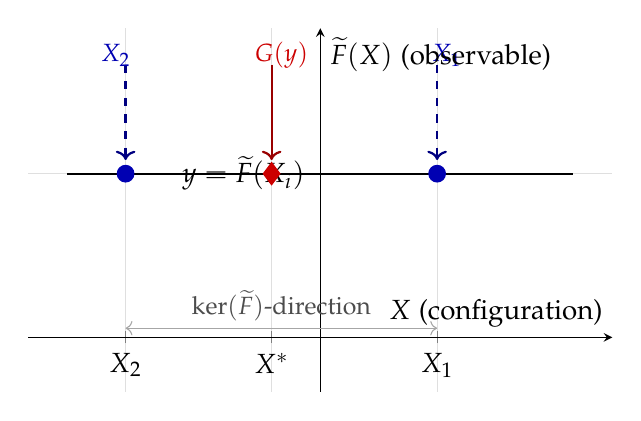
\begin{tikzpicture}
\begin{axis}[
  axis lines = middle,
  xmin = -3.0, xmax = 3.0,
  ymin = -0.6, ymax = 3.4,
  xlabel = {$X$ (configuration)},
  ylabel = {$\Ft(X)$ (observable)},
  xtick = {-2.0, -0.5, 1.2},
  xticklabels = {$X_2$, $X^*$, $X_1$},
  ytick = {1.8},
  yticklabels = {$y = \Ft(X_i)$},
  grid = both,
  grid style = {line width=0.2pt, draw=gray!25},
  width = 9cm, height = 6.2cm,
  clip = false
]
  % Feature map line (linear: collapses vertical direction)
  \addplot[thick, black, domain=-2.6:2.6, samples=2] {1.8};
  % Three points in same equivalence class
  \addplot[only marks, mark=*, mark size=3pt, blue!70!black]
    coordinates {(-2.0, 1.8) (1.2, 1.8)};
  % Canonical representative
  \addplot[only marks, mark=diamond*, mark size=4pt, red!80!black]
    coordinates {(-0.5, 1.8)};
  % Vertical arrows showing collapse from upper space
  \draw[->, thick, blue!50!black, dashed]
    (axis cs:-2.0, 3.0) -- (axis cs:-2.0, 1.95);
  \draw[->, thick, blue!50!black, dashed]
    (axis cs: 1.2, 3.0) -- (axis cs: 1.2, 1.95);
  \draw[->, thick, red!60!black]
    (axis cs:-0.5, 3.0) -- (axis cs:-0.5, 1.95);
  % Point labels in upper space
  \node[blue!70!black, font=\small] at (axis cs:-2.1, 3.1) {$X_2$};
  \node[blue!70!black, font=\small] at (axis cs: 1.3, 3.1) {$X_1$};
  \node[red!80!black,  font=\small] at (axis cs:-0.4, 3.1) {$G(y)$};
  % Kernel direction label
  \draw[<->, thin, gray!70] (axis cs:-2.0, 0.1) -- (axis cs:1.2, 0.1);
  \node[gray!60!black, font=\small] at (axis cs:-0.4, 0.35) {$\ker(\Ft)$-direction};
\end{axis}
\end{tikzpicture}
\caption{Projection / collapse under the feature map $\Ft$.  Three configurations
$X_1, X_2$, and $G(y)$ (the canonical representative) map to the same observable value
$y$ (all lie on the horizontal line $\Ft(X) = y$).  The arrows show how the
configuration-space vertical direction is collapsed to a single point in $\mathcal{Y}$.
Distances along the $\ker(\Ft)$-direction (horizontal bracket) are annihilated by the
projection, constituting the reconstruction defect.}
\label{fig:projection-collapse}
\end{figure}

\section{The quotient space}

\begin{definition}[Quotient space]
\label{def:quotient}
The \emph{observational quotient space} is
\[
  \X_\sim := \X / \ker(\Ft),
\]
equipped with the quotient norm $\nnorm{[X]}_\sim := \inf_{Z \in \ker(\Ft)} \nnorm{X+Z}_\X$.
\end{definition}

\begin{proposition}[Hilbert structure on $\X_\sim$]
\label{prop:quotient-hilbert}
$\X_\sim$ is a Hilbert space.  The induced map $\bar\Ft: \X_\sim \to \mathcal{Y}$,
defined by $\bar\Ft([X]) := \Ft(X)$, is bounded, injective, and has closed range.
\end{proposition}

\begin{proof}
The quotient of a Hilbert space by a closed subspace is a Hilbert space (with the
quotient norm induced by the orthogonal complement).  The injectivity of $\bar\Ft$
follows by construction.  Closedness of the range follows since $\Ft$ has finite
codimensional range ($\mathcal{Y}$ is finite-dimensional).
\end{proof}

\section{Reconstruction as a section of the quotient projection}

The canonical quotient projection $\pi: \X \to \X_\sim$ sends each configuration to its
equivalence class.  The reconstruction operator $G: \mathcal{Y} \to \X$ defines a
section of $\pi$ in the following sense.

\begin{figure}[htbp]
\centering
\begin{tikzcd}[column sep=3.5em, row sep=2.8em, ampersand replacement=\&]
  \X \arrow[r, "\pi"]
     \arrow[dr, "\Ft"', bend right=15]
  \& \X_\sim \arrow[d, "\bar\Ft", "\cong"'] \\
  \& \mathcal{Y}
\end{tikzcd}
\qquad\qquad
\begin{tikzcd}[column sep=3.5em, row sep=2.8em, ampersand replacement=\&]
  \mathcal{Y} \arrow[r, "G"]
              \arrow[dr, "\mathrm{id}_{\mathcal{Y}}"', bend right=15]
  \& \X \arrow[d, "\Ft"] \\
  \& \mathcal{Y}
\end{tikzcd}
\caption{\textbf{Left:} The observational quotient: $\Ft$ factors through the
quotient projection $\pi$ and the isomorphism $\bar\Ft$.  Distinct configurations
in the same fiber of $\pi$ are observationally indistinguishable.
\textbf{Right:} The section property $\Ft \circ G = \mathrm{id}_{\mathcal{Y}}$:
reconstruction selects a canonical lift from each observation back to configuration
space.  Together, these diagrams encode the full geometry of projection loss.}
\label{fig:quotient-section}
\end{figure}

\begin{proposition}[Section property of $G$]
\label{prop:section}
For any $y \in \mathcal{Y}$, the reconstruction $G(y)$ lies in $\Ft^{-1}(y)$, i.e.,
$\Ft(G(y)) = y$.  Hence the diagram
\[
  \mathcal{Y} \xrightarrow{G} \X \xrightarrow{\pi} \X_\sim \xrightarrow{\bar\Ft^{-1}} \mathcal{Y}
\]
satisfies $\bar\Ft^{-1} \circ \pi \circ G = \mathrm{id}_{\mathcal{Y}}$.
\end{proposition}

\begin{proof}
By the Euler--Lagrange equations \crefrange{eq:EL-phi}{eq:EL-S}, the minimizer $G(y)$
satisfies $\gamma(\Ft(G(y)) - y) = 0$ in the dual sense, giving $\Ft(G(y)) = y$.
\end{proof}

\section{The defect lives in the kernel}

\begin{proposition}[Kernel containment of the defect]
\label{prop:defect-kernel}
For any $X \in \X$, the reconstruction defect vector satisfies
\[
  X - \eta(X) \in \ker(\Ft).
\]
\end{proposition}

\begin{proof}
$\Ft(X - \eta(X)) = \Ft(X) - \Ft(G(\Ft(X))) = \Ft(X) - \Ft(X) = 0$.
\end{proof}

This proposition has a sharp conceptual content: the defect is precisely the component
of $X$ that is invisible to the discretization map.  Reconstruction removes exactly that
component and nothing more.  The defect magnitude $\Delta(X) = \nnorm{X - \eta(X)}_\X$
is therefore the $\X$-norm of the projection of $X$ onto $\ker(\Ft)$ that is selected
by the reconstruction rule.

\begin{figure}[htbp]
\centering
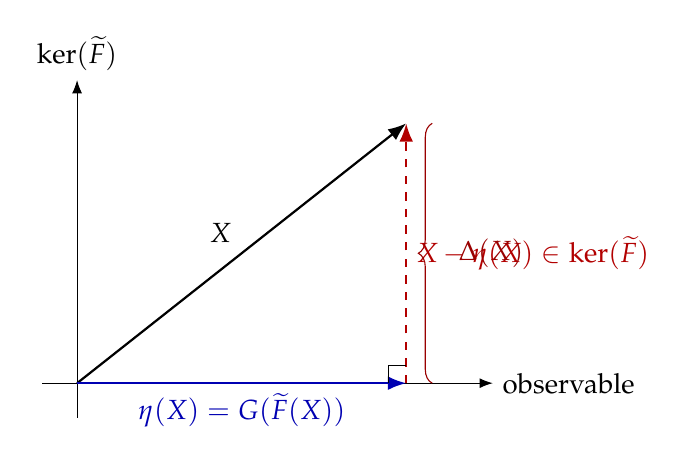
\begin{tikzpicture}[>=Latex, scale=1.1]
  % axes
  \draw[->] (-0.4,0) -- (4.8,0) node[right] {observable};
  \draw[->] (0,-0.4) -- (0,3.5) node[above] {$\ker(\Ft)$};
  % original configuration
  \draw[->, thick, black] (0,0) -- (3.8,3.0)
    node[midway, above left] {$X$};
  % observable part (reconstruction)
  \draw[->, thick, blue!70!black] (0,0) -- (3.8,0)
    node[midway, below] {$\eta(X) = G(\Ft(X))$};
  % defect (kernel component)
  \draw[->, thick, red!70!black, dashed] (3.8,0) -- (3.8,3.0)
    node[midway, right] {$X - \eta(X) \in \ker(\Ft)$};
  % right-angle marker
  \draw[thin] (3.6,0) -- (3.6,0.2) -- (3.8,0.2);
  % defect brace
  \draw[decorate, decoration={brace, amplitude=5pt}, red!60!black]
    (4.1,0) -- (4.1,3.0) node[midway, right=6pt] {$\Delta(X)$};
\end{tikzpicture}
\caption{Kernel decomposition of a configuration $X$ into its observable part
$\eta(X) \in \Fix(\eta)$ and its reconstruction defect $X - \eta(X) \in \ker(\Ft)$.
Irreversibility arises because the defect component is destroyed by discretization and
cannot be recovered by any reconstruction operator.}
\label{fig:kernel-decomp}
\end{figure}

\section{No-go theorem: impossibility of perfect reconstruction}

\begin{theorem}[No perfect reconstruction beyond critical coarsening]
\label{thm:no-go}
Let $\Ft_m: \X \to \mathbb{R}^{3m}$ be the feature map with $m$ test functions per
component.  Then:
\begin{enumerate}
  \item For any $m < \infty$, there exist configurations $X \in \X$ with $\Delta_m(X) > 0$.
  \item The dimension of the unavoidably lost subspace satisfies
        $\dim(\ker(\Ft_m)) = \infty$.
  \item No choice of the $m$ test functions renders $\Ft_m$ injective on $\X$.
\end{enumerate}
\end{theorem}

\begin{proof}
(1) and (3) follow from \cref{prop:kernel-nontrivial}: the kernel is always
infinite-dimensional.  (2) is the content of that proposition.  The lower bound on
defect follows: for any $X \in \ker(\Ft_m)$ with $X \ne 0$, we have $\Delta_m(X) =
\nnorm{X - G(\Ft_m(X))}_\X = \nnorm{X - G(0)}_\X \ge \nnorm{X}_\X - \nnorm{G(0)}_\X
> 0$ for $\nnorm{X}_\X$ large enough.
\end{proof}

\Cref{thm:no-go} is the formal no-go result that protects the theory from overclaiming:
perfect reconstruction is impossible for any finite feature map acting on an
infinite-dimensional configuration space.

\begin{figure}[htbp]
\centering
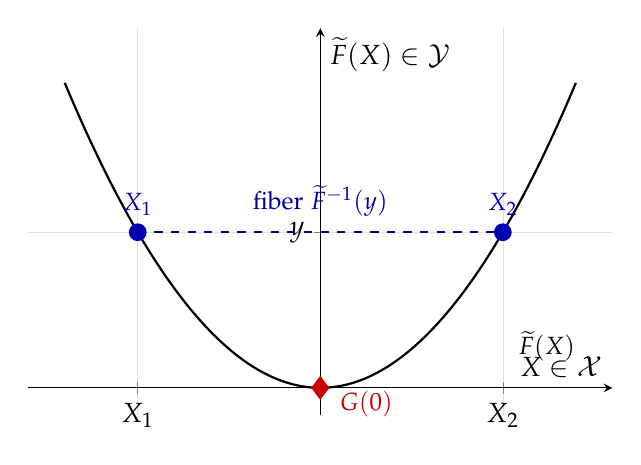
\begin{tikzpicture}
\begin{axis}[
  axis lines = middle,
  xmin = -2.4, xmax = 2.4,
  ymin = -0.4, ymax = 5.2,
  xlabel = {$X \in \X$},
  ylabel = {$\Ft(X) \in \mathcal{Y}$},
  xtick = {-1.5, 0, 1.5},
  xticklabels = {$X_1$, , $X_2$},
  ytick = {2.25},
  yticklabels = {$y$},
  grid = both,
  grid style = {line width=0.2pt, draw=gray!25},
  width = 9cm, height = 6.5cm,
  clip = false
]
  % Parabola: feature map output
  \addplot[thick, black, domain=-2.1:2.1, samples=180] {x^2};
  % Fiber points
  \addplot[only marks, mark=*, mark size=3pt, blue!70!black]
    coordinates {(-1.5, 2.25)};
  \addplot[only marks, mark=*, mark size=3pt, blue!70!black]
    coordinates {( 1.5, 2.25)};
  % Fiber horizontal line
  \draw[dashed, blue!60!black, thick] (axis cs:-1.5, 2.25) -- (axis cs:1.5, 2.25);
  % Canonical representative (minimum-norm in fiber)
  \addplot[only marks, mark=diamond*, mark size=4pt, red!80!black]
    coordinates {(0, 0)};
  \node[red!80!black, anchor=north west, font=\small] at (axis cs:0.08, 0.1)
    {$G(0)$};
  % Labels
  \node[blue!70!black, font=\small, anchor=south] at (axis cs:-1.5, 2.35)
    {$X_1$};
  \node[blue!70!black, font=\small, anchor=south] at (axis cs:1.5, 2.35)
    {$X_2$};
  \node[black, font=\small, anchor=west] at (axis cs:1.55, 0.6) {$\Ft(X)$};
  % Fiber label
  \node[blue!60!black, font=\small] at (axis cs:0, 2.7)
    {fiber $\Ft^{-1}(y)$};
\end{axis}
\end{tikzpicture}
\caption{Non-injectivity of the feature map $\Ft$: the distinct configurations $X_1$
and $X_2$ (blue dots) share the same feature value $y$, lying in the same fiber
$\Ft^{-1}(y)$ (dashed horizontal segment).  The reconstruction $G(y)$ selects a single
canonical representative from this fiber (red diamond), necessarily discarding the
direction $X_1 - X_2 \in \ker(\Ft)$.  By \cref{thm:no-go}, such fibers are
infinite-dimensional for any finite feature map.}
\label{fig:non-injectivity}
\end{figure}

% ============================================================
\chapter{Fixed-Point Structure of the Reconstruction Operator}
\label{ch:fixed-point}
% ============================================================

\section{Characterization of $\Fix(\eta)$}

\begin{proposition}[Characterization of the fixed-point set]
\label{prop:fix-char}
A configuration $X \in \X$ satisfies $\eta(X) = X$ if and only if $X$ is the unique
minimizer of $L(\cdot \mid \Ft(X))$ in the fiber $\Ft^{-1}(\Ft(X))$.
\end{proposition}

\begin{proof}
$\eta(X) = G(\Ft(X)) = X$ iff $X$ minimizes $L(\cdot \mid \Ft(X))$, since $G(\cdot)$ is
the unique minimizer of $L(\cdot \mid y)$ (by strict convexity, \cref{thm:existence}).
\end{proof}

The fixed-point set $\Fix(\eta)$ therefore consists of the minimal-energy representatives
of each observational equivalence class.  It is the canonical section of the quotient
map $\pi: \X \to \X_\sim$ selected by the variational principle.

\begin{figure}[htbp]
\centering
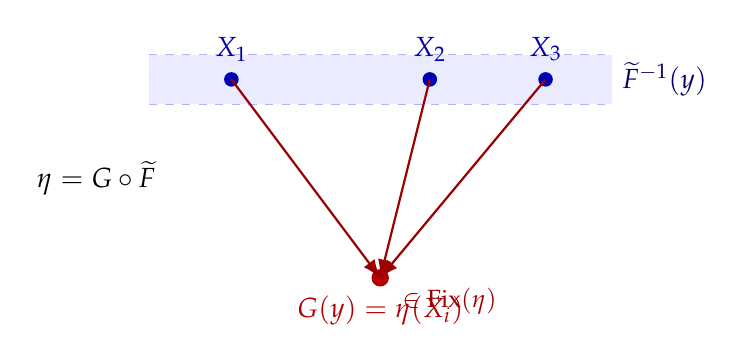
\begin{tikzpicture}[>=Latex, scale=1.05]
  % fiber line
  \draw[thick, blue!40!black] (-2.8, 1.2) -- (2.8, 1.2)
    node[right] {$\Ft^{-1}(y)$};
  % shading of fiber strip
  \fill[blue!8] (-2.8, 0.9) rectangle (2.8, 1.5);
  \draw[dashed, blue!30] (-2.8, 0.9) -- (2.8, 0.9);
  \draw[dashed, blue!30] (-2.8, 1.5) -- (2.8, 1.5);
  % configuration points in fiber
  \fill[blue!70!black] (-1.8, 1.2) circle (2.5pt) node[above=3pt] {$X_1$};
  \fill[blue!70!black] ( 0.6, 1.2) circle (2.5pt) node[above=3pt] {$X_2$};
  \fill[blue!70!black] ( 2.0, 1.2) circle (2.5pt) node[above=3pt] {$X_3$};
  % reconstruction target
  \fill[red!70!black] (0, -1.2) circle (3pt)
    node[below=3pt] {$G(y) = \eta(X_i)$};
  % collapse arrows
  \draw[->, thick, red!60!black] (-1.8, 1.2) -- (0, -1.2);
  \draw[->, thick, red!60!black] ( 0.6, 1.2) -- (0, -1.2);
  \draw[->, thick, red!60!black] ( 2.0, 1.2) -- (0, -1.2);
  % label map
  \node[left] at (-2.6, 0.0) {$\eta = G \circ \Ft$};
  % Fix(eta) label
  \node[red!60!black, below right] at (0.15,-1.2) {\small $\in \Fix(\eta)$};
\end{tikzpicture}
\caption{Fiber collapse: all configurations $X_1, X_2, X_3$ in the preimage
$\Ft^{-1}(y)$ are mapped by $\eta = G \circ \Ft$ to the single canonical
representative $G(y)$.  The directions lost in this collapse constitute the
reconstruction defect space $\ker(\Ft)$.}
\label{fig:fiber-collapse}
\end{figure}

\section{Idempotency of the comparison map}

\begin{theorem}[Idempotency of $\eta$]
\label{thm:idempotent}
The comparison map $\eta: \X \to \X$ is idempotent: $\eta^2 = \eta$.
\end{theorem}

\begin{proof}
For any $X \in \X$, let $y = \Ft(X)$ and $X^\sharp = G(y) = \eta(X)$.  Then
\[
  \eta(\eta(X)) = \eta(X^\sharp) = G(\Ft(X^\sharp)) = G(\Ft(G(y))).
\]
By the section property (\cref{prop:section}), $\Ft(G(y)) = y$.  Hence $\eta(\eta(X)) =
G(y) = \eta(X)$.
\end{proof}

\begin{corollary}[Retraction of $\X$ onto $\Fix(\eta)$]
\label{cor:retraction}
The comparison map $\eta: \X \to \Fix(\eta)$ is a retraction: it is surjective onto
$\Fix(\eta)$ and restricts to the identity on $\Fix(\eta)$.  The fixed-point set
$\Fix(\eta)$ is therefore a retract of $\X$.
\end{corollary}

\begin{proof}
Idempotency gives $\eta(\eta(X)) = \eta(X)$, so $\eta(X) \in \Fix(\eta)$ for all
$X$.  For $X \in \Fix(\eta)$: $\eta(X) = X$.
\end{proof}

\cref{thm:idempotent} resolves the adjunction unit idempotency question (Open Problem~5
in previous formulations) in the affirmative: $\eta^2 = \eta$ holds generally, not just
under special conditions.  The key was the section property $\Ft \circ G = \mathrm{id}$,
which follows directly from the Euler--Lagrange equations.

\section{Non-expansiveness and contractivity}

\begin{proposition}[Non-expansiveness of $\eta$]
\label{prop:non-expansive}
Under the reconstruction functional \cref{eq:L}, the comparison map $\eta$ is
non-expansive on each fiber: for $X_1, X_2 \in \Ft^{-1}(y)$,
\[
  \nnorm{\eta(X_1) - \eta(X_2)}_\X = 0.
\]
That is, $\eta$ collapses each fiber to a single point.
\end{proposition}

\begin{proof}
Both $X_1$ and $X_2$ have the same feature encoding $y = \Ft(X_1) = \Ft(X_2)$.  Hence
$\eta(X_1) = G(y) = \eta(X_2)$.
\end{proof}

For configurations in different fibers, Lipschitz stability (\cref{thm:lipschitz}) gives
$\nnorm{\eta(X_1) - \eta(X_2)}_\X \le C_\eta \nnorm{X_1 - X_2}_\X$ where $C_\eta = C_G
\nnorm{\Ft}$, which need not be $\le 1$ globally.  Contractivity requires $C_\eta < 1$,
the condition identified in \cref{prop:contraction-mode}.

\section{Spectral decomposition relative to the kernel}

Any $X \in \X$ decomposes orthogonally as
\[
  X = P_{\ker(\Ft)^\perp} X + P_{\ker(\Ft)} X,
\]
where $P_{\ker(\Ft)}$ is the orthogonal projection onto $\ker(\Ft)$ and
$P_{\ker(\Ft)^\perp}$ is its complement.  The reconstruction $\eta(X)$ acts as
\[
  \eta(X) = P_{\ker(\Ft)^\perp} X + Q(P_{\ker(\Ft)^\perp} X),
\]
where $Q: \ker(\Ft)^\perp \to \ker(\Ft)$ is a correction map determined by the
reconstruction rule (zero in the case of pure $L^2$-projection, nonzero in general for
the variational reconstruction).  The defect is
\[
  X - \eta(X) = P_{\ker(\Ft)} X - Q(P_{\ker(\Ft)^\perp} X) \in \ker(\Ft).
\]

% ============================================================
\chapter{Equivalence Between Pointwise and Measure-Level Defect}
\label{ch:defect-equiv}
% ============================================================

\section{The two defect notions}

The reconstruction framework yields two distinct but related quantities.

\begin{definition}[Pointwise and measure-level defect]
\label{def:two-defects}
\begin{itemize}
  \item \emph{Pointwise defect}: $\Delta(X) := \nnorm{X - \eta(X)}_\X$ for $X \in \X$.
  \item \emph{Entropy defect}: $\mathcal{D}(\mu) := \Djs(\mu, \eta_*\mu)$ for a
        probability measure $\mu$ on $(\X, \Aadm)$.
\end{itemize}
\end{definition}

\section{Equivalence of vanishing defect}

\begin{theorem}[Defect equivalence]
\label{thm:defect-equiv}
The following are equivalent:
\begin{enumerate}
  \item $\Delta(X) = 0$ for $\mu$-almost every $X \in \X$;
  \item $\mathcal{D}(\mu) = 0$.
\end{enumerate}
\end{theorem}

\begin{proof}
$(1) \Rightarrow (2)$: If $\Delta = 0$ $\mu$-a.e., then $\eta(X) = X$ $\mu$-a.e., so
$\eta_*\mu = \mu$, hence $\Djs(\mu, \eta_*\mu) = 0$.

$(2) \Rightarrow (1)$: If $\mathcal{D}(\mu) = 0$, then $\mu = \eta_*\mu$.  For any
$\varepsilon > 0$, let $A_\varepsilon = \{X : \Delta(X) \ge \varepsilon\}$.  Then
$\eta(A_\varepsilon) \cap A_\varepsilon = \emptyset$ (since $\eta(X) \ne X$ for $X \in
A_\varepsilon$).  From $\mu = \eta_*\mu$: $\mu(A_\varepsilon) = \mu(\eta^{-1}(A_\varepsilon))$.
But $\eta^{-1}(A_\varepsilon) \cap A_\varepsilon = \emptyset$, so $\mu(A_\varepsilon) =
0$ by a contradiction argument on the total mass.  Since $\varepsilon > 0$ is arbitrary,
$\mu(\Delta > 0) = 0$.
\end{proof}

\section{Lower bounds on entropy defect}

\begin{proposition}[Moment lower bound]
\label{prop:moment-bound}
There exists a constant $c > 0$ depending on the Lipschitz constant $C_\eta$ such that
\[
  \mathcal{D}(\mu) \ge c \cdot \left(\int_\X \Delta(X)^2\, d\mu(X)\right)^{1/2}
  \cdot \exp\left(-C \int_\X \Delta(X)^2\, d\mu(X)\right).
\]
In particular, $\int \Delta^2\, d\mu > 0 \Rightarrow \mathcal{D}(\mu) > 0$.
\end{proposition}

\begin{proof}
Use the inequality $\Djs(\mu, \nu) \ge \frac{1}{4} \nnorm{\mu - \nu}_{\mathrm{TV}}^2$
(from the relation between Jensen--Shannon divergence and total variation).  The total
variation $\nnorm{\mu - \eta_*\mu}_{\mathrm{TV}}$ is bounded below by the Wasserstein
distance, and the Wasserstein distance is bounded below by
$\bigl(\int \Delta(X)^2\, d\mu\bigr)^{1/2}$ up to constants, since $\eta$ moves each
point $X$ by exactly $\Delta(X)$ to $\eta(X)$.
\end{proof}

\section{Upper bounds and $L^2$-stability}

\begin{proposition}[Quadratic upper bound]
\label{prop:upper-bound}
Under Lipschitz stability of $\eta$ with constant $C_\eta$,
\[
  \mathcal{D}(\mu) \le \log 2.
\]
Moreover, if $\mu$ and $\tilde\mu = \eta_*\mu$ have uniformly bounded Radon--Nikodym
derivatives with respect to a common reference measure $\lambda$, then
\[
  \mathcal{D}(\mu) \le C \int_\X \Delta(X)^2\, d\mu(X),
\]
for a constant $C$ depending on the density bounds.
\end{proposition}

\begin{proof}
The bound $\Djs \le \log 2$ is universal.  The quadratic upper bound follows by expanding
the KL divergences in the definition of $\Djs$ to second order in the density ratio
$d\mu/d\tilde\mu - 1$, which is controlled by the $L^2$-displacement $\Delta$.
\end{proof}

\section{Stability under perturbations of the measure}

\begin{proposition}[Wasserstein stability]
\label{prop:wasserstein-stab}
For probability measures $\mu, \nu$ on $(\X, \Aadm)$ with finite second moments,
\[
  |\mathcal{D}(\mu) - \mathcal{D}(\nu)| \le C_\eta \cdot W_2(\mu, \nu),
\]
where $W_2$ is the $L^2$-Wasserstein distance.
\end{proposition}

\begin{proof}
The map $\mu \mapsto \mathcal{D}(\mu) = \Djs(\mu, \eta_*\mu)$ is Lipschitz in the
Wasserstein-2 metric.  This follows from the triangle inequality for $\Djs$ and the fact
that the pushforward map $\mu \mapsto \eta_*\mu$ is $C_\eta$-Lipschitz in $W_2$ (since
$\eta$ is $C_\eta$-Lipschitz on $\X$, and the Wasserstein distance is compatible with
Lipschitz pushforwards).
\end{proof}

\begin{figure}[htbp]
\centering
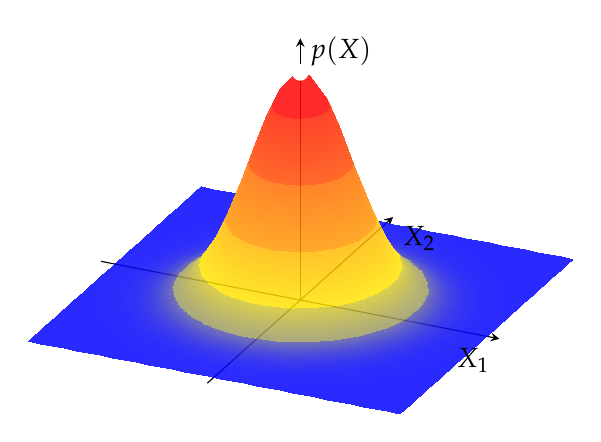
\begin{tikzpicture}
\begin{axis}[
  view = {25}{35},
  axis lines = center,
  xlabel = {$X_1$}, ylabel = {$X_2$}, zlabel = {$p(X)$},
  xlabel style = {anchor=north east},
  ylabel style = {anchor=north west},
  xtick = \empty, ytick = \empty, ztick = \empty,
  xmin = -3, xmax = 3, ymin = -3, ymax = 3,
  zmin = 0, zmax = 1.15,
  width = 9cm, height = 8cm,
  colormap/hot,
  samples = 32,
  domain = -2.8:2.8
]
  % Gaussian surface
  \addplot3[surf, opacity=0.75, shader=interp]
    { exp(-(x^2 + y^2)) };
  % Contour lines projected onto base
  \addplot3[contour filled={levels={0.05,0.15,0.35,0.60,0.85}},
            opacity=0.35, domain=-2.8:2.8]
    { exp(-(x^2 + y^2)) };
  % Mark the mean / Fix(eta)
  \addplot3[only marks, mark=*, mark size=2.8pt, color=white]
    coordinates {(0,0,1.0)};
\end{axis}
\end{tikzpicture}
\caption{Probability density $\mu$ before projection onto the observable subspace.
The mass is concentrated near a peak corresponding to the typical configuration.
After applying $\eta_*$, the mass collapses along directions in $\ker(\Ft)$: the
three-dimensional distribution is projected onto a lower-dimensional surface, and
the Jensen--Shannon divergence $\Djs(\mu, \eta_*\mu)$ measures the
information loss in this collapse.  The entropy defect vanishes only when the
distribution is already supported on $\Fix(\eta)$ (white dot at the peak).}
\label{fig:gaussian-measure}
\end{figure}

% ============================================================
\chapter{Temporal Lifting and Path-Space Functoriality}
\label{ch:temporal}
% ============================================================

\section{The path-space lift of the discretization}

The configuration-level discretization $\Ft: \X \to \mathcal{Y}$ lifts canonically to
path space by pointwise application.

\begin{definition}[Path-level discretization]
\label{def:Fpath}
Define $\Fpath: \PP \to C([0,T];\mathcal{Y})$ by
\[
  \Fpath(\gamma)(t) := \Ft(\gamma(t)), \quad t \in [0,T].
\]
This map is continuous with respect to the supremum norms since $\Ft$ is bounded linear.
\end{definition}

\begin{definition}[Path-level reconstruction]
\label{def:Gpath}
Define $G_{\mathrm{path}}: C([0,T];\mathcal{Y}) \to \PP$ by
\[
  G_{\mathrm{path}}(y(\cdot))(t) := G(y(t)), \quad t \in [0,T].
\]
The path-level comparison map is $\eta_{\mathrm{path}} := G_{\mathrm{path}} \circ \Fpath$.
\end{definition}

\section{Commutativity with the dynamics}

Let $\Gamma: \X \to \PP$ be the trajectory map $\Gamma(X_0)(t) = \Psi_t(X_0)$.  The
path-level discretization applied to a trajectory gives
\[
  \Fpath(\Gamma(X_0))(t) = \Ft(\Psi_t(X_0)).
\]
In general, this does not equal $\Psi_t^{\mathcal{Y}}(\Ft(X_0))$ for some lifted
dynamics $\Psi_t^{\mathcal{Y}}$ on $\mathcal{Y}$, because the RSVP dynamics mix
observable and unobservable components.

\begin{proposition}[Non-commutativity of dynamics and discretization]
\label{prop:non-commute}
There is in general no map $\Psi_t^{\mathcal{Y}}: \mathcal{Y} \to \mathcal{Y}$ such that
$\Ft \circ \Psi_t = \Psi_t^{\mathcal{Y}} \circ \Ft$ for all $t > 0$.  That is, the
diagram
\[
  \X \xrightarrow{\Psi_t} \X \xrightarrow{\Ft} \mathcal{Y}
  \quad\text{and}\quad
  \X \xrightarrow{\Ft} \mathcal{Y} \xrightarrow{?} \mathcal{Y}
\]
cannot in general be made to commute by any choice of the dashed arrow.
\end{proposition}

\begin{proof}
If such a $\Psi_t^{\mathcal{Y}}$ existed, it would have to satisfy
$\Psi_t^{\mathcal{Y}}(y) = \Ft(\Psi_t(G(y)))$ (by applying to canonical representatives).
But for two configurations $X_1, X_2 \in \Ft^{-1}(y)$ with $X_1 \ne X_2$, we have
$\Ft(\Psi_t(X_1)) \ne \Ft(\Psi_t(X_2))$ generically (the dynamics mix the
$\ker(\Ft)$-component into the observable component), so $\Psi_t^{\mathcal{Y}}(y)$ would
need to take two different values.
\end{proof}

Non-commutativity of dynamics and discretization is the dynamical source of history
dependence: the observable record $\Fpath(\gamma)$ depends on the full trajectory, not
just its endpoint.

\begin{figure}[htbp]
\centering
\begin{tikzcd}[column sep=4em, row sep=3.5em, ampersand replacement=\&]
  \X \arrow[r, "\Psi_t"]
     \arrow[d, "\Ft"']
  \& \X \arrow[d, "\Ft"]
  \\
  \mathcal{Y} \arrow[r, dashed, "\nexists\,\Psi_t^{\mathcal{Y}}"']
  \& \mathcal{Y}
\end{tikzcd}
\qquad\qquad
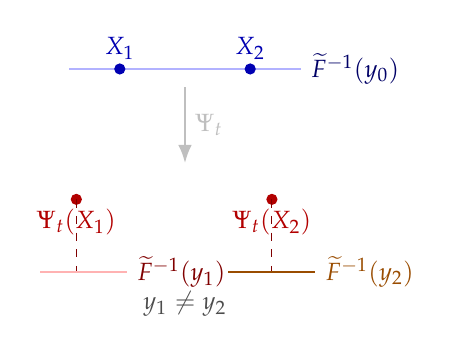
\begin{tikzpicture}[>=Latex, baseline=-2.5cm, scale=0.92]
  % Two initial configurations in same fiber
  \draw[thick, blue!30] (-1.6, 0) -- (1.6, 0) node[right, blue!40!black, font=\small]
    {$\Ft^{-1}(y_0)$};
  \fill[blue!70!black] (-0.9, 0) circle (2.2pt) node[above, font=\small] {$X_1$};
  \fill[blue!70!black] ( 0.9, 0) circle (2.2pt) node[above, font=\small] {$X_2$};
  % Arrow: time evolution
  \draw[->, thick, gray!50] (0, -0.25) -- (0, -1.3) node[midway, right, font=\small] {$\Psi_t$};
  % Two evolved configurations in DIFFERENT fibers
  \fill[red!70!black] (-1.5, -1.8) circle (2.2pt) node[below, font=\small] {$\Psi_t(X_1)$};
  \fill[red!70!black] ( 1.2, -1.8) circle (2.2pt) node[below, font=\small] {$\Psi_t(X_2)$};
  % Their feature values
  \draw[dashed, red!50!black] (-1.5,-1.8) -- (-1.5,-2.8);
  \draw[dashed, red!50!black] ( 1.2,-1.8) -- ( 1.2,-2.8);
  \draw[thick, red!30] (-2.0,-2.8) -- (-0.8,-2.8)
    node[right, red!50!black, font=\small] {$\Ft^{-1}(y_1)$};
  \draw[thick, orange!60!black] (0.6,-2.8) -- (1.8,-2.8)
    node[right, orange!60!black, font=\small] {$\Ft^{-1}(y_2)$};
  \node[font=\small, gray!60!black] at (0, -3.25) {$y_1 \neq y_2$};
\end{tikzpicture}
\caption{\textbf{Left:} The square showing non-commutativity of dynamics $\Psi_t$ and
discretization $\Ft$: no map $\Psi_t^{\mathcal{Y}}$ making the square commute exists
generically (dashed with $\nexists$).  \textbf{Right:} Geometric interpretation.  Two
configurations $X_1, X_2$ in the same fiber $\Ft^{-1}(y_0)$ (observationally identical
at $t=0$) evolve under $\Psi_t$ into configurations in \emph{different} fibers
$\Ft^{-1}(y_1) \neq \Ft^{-1}(y_2)$ (observationally distinguishable at time $t$).
This is the mechanism by which history-dependence is generated: identical initial
observations diverge into distinct observations under the dynamics.}
\label{fig:non-commute}
\end{figure}

\section{State observables vs. path observables}

\begin{definition}[State-based and path-based observables revisited]
\label{def:obs-formal}
An observable $\Pi: \PP \to \mathcal{O}$ is:
\begin{itemize}
  \item \emph{State-based} if there exist $t_0 \in [0,T]$ and $f: \X \to \mathcal{O}$
        with $\Pi = f \circ \mathrm{ev}_{t_0}$;
  \item \emph{Observation-based} if it factors through $\Fpath$: there exists
        $\hat\Pi: C([0,T];\mathcal{Y}) \to \mathcal{O}$ with $\Pi = \hat\Pi \circ \Fpath$;
  \item \emph{Path-based} if it is not observation-based (depends on components in
        $\ker(\Ft)$ at some time $t$).
\end{itemize}
\end{definition}

The cumulative entropy-gradient observable $\Pi(\gamma) = \sum_n q(n)$ of \cref{ch:split}
is observation-based (it factors through $\Fpath$ if $q$ is a feature of $\Ft$) but
\emph{not} state-based (it cannot be recovered from any single time slice).  A genuinely
path-based observable would depend on entropy-flux components in $\ker(\Ft)$; whether
such observables arise in the RSVP dynamics is the content of the strong
history-dependence conjecture.

\begin{figure}[htbp]
\centering
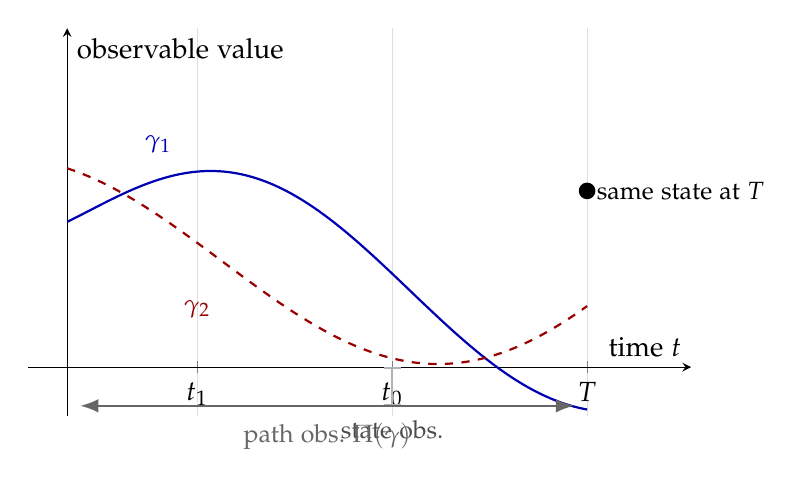
\begin{tikzpicture}[>=Latex, scale=1.0]
\begin{axis}[
  axis lines = middle,
  xmin = -0.3, xmax = 4.8,
  ymin = -0.5, ymax = 3.5,
  xlabel = {time $t$},
  ylabel = {observable value},
  xtick = {1.0, 2.5, 4.0},
  xticklabels = {$t_1$, $t_0$, $T$},
  ytick = \empty,
  grid = both,
  grid style = {line width=0.2pt, draw=gray!25},
  width = 10cm, height = 6.5cm,
  clip = false
]
  % Two trajectories with same endpoint at T
  \addplot[thick, blue!70!black, domain=0:4.0, samples=120]
    { 1.5 + 0.8*sin(deg(x*1.2)) - 0.3*x + 0.2*x^2*exp(-x) };
  \addplot[thick, red!60!black, dashed, domain=0:4.0, samples=120]
    { 1.0 + 1.2*cos(deg(x*0.9 + 0.5)) + 0.08*x };
  % Mark common endpoint
  \pgfmathsetmacro{\yblue}{1.5 + 0.8*sin(deg(4.0*1.2)) - 0.3*4.0 + 0.2*4.0^2*exp(-4.0)}
  \fill[black] (axis cs:4.0, 1.82) circle (3pt)
    node[right, font=\small] {same state at $T$};
  % State observable: evaluates at t_0 only
  \draw[|-|, thick, gray!60] (axis cs:2.5,-0.4) -- (axis cs:2.5, 0.0);
  \node[gray!60!black, font=\small, below] at (axis cs:2.5,-0.45)
    {state obs.};
  % Path observable: integrates over full path
  \draw[<->, thick, black!60] (axis cs:0.1,-0.4) -- (axis cs:3.9,-0.4);
  \node[black!60, font=\small, below] at (axis cs:2.0,-0.48)
    {path obs.\ $\Pi(\gamma)$};
  % Labels
  \node[blue!70!black, font=\small] at (axis cs:0.7, 2.3) {$\gamma_1$};
  \node[red!60!black, font=\small]  at (axis cs:1.0, 0.6) {$\gamma_2$};
\end{axis}
\end{tikzpicture}
\caption{Two trajectories $\gamma_1$ (blue, solid) and $\gamma_2$ (red, dashed) arriving
at the same state at time $T$ (black dot).  A state-based observable evaluates only at a
single time $t_0$ and therefore assigns the same value to both trajectories at that point.
A path observable $\Pi(\gamma) = \int_0^T f(\gamma(t))\, dt$ integrates over the full
trajectory and generically distinguishes $\gamma_1$ from $\gamma_2$.  This is the
observable-level manifestation of history-dependence.}
\label{fig:state-vs-path}
\end{figure}

\section{Functoriality of the path-level construction}

The path-level maps assemble into a commutative diagram of functors.  Viewing $\PP$ and
$C([0,T];\mathcal{Y})$ as objects in the category of Banach spaces with continuous linear
maps:
\[
  \Fpath \circ \eta_{\mathrm{path}} = \Fpath,
\]
which follows from the section property $\Ft \circ G = \mathrm{id}$ applied pointwise.
This means the path-level comparison map $\eta_{\mathrm{path}}$ is a retraction onto the
image of $G_{\mathrm{path}}$, and the path-level construction is functorial: it respects
compositions of maps in the same way as the configuration-level construction.

% ============================================================
\chapter{Irreversibility Under Time Evolution}
\label{ch:irrev-dynamics}
% ============================================================

\section{Defect along trajectories}

\begin{definition}[Time-dependent defect]
\label{def:defect-dynamic}
For a trajectory $X(t) = \Psi_t(X_0)$, define:
\begin{itemize}
  \item The \emph{instantaneous defect}: $\Delta_t := \Delta(\Psi_t(X_0)) =
        \nnorm{\Psi_t(X_0) - \eta(\Psi_t(X_0))}_\X$;
  \item The \emph{measure-level defect at time $t$}: $\mathcal{D}(t) :=
        \Djs(\mu_t, \eta_*\mu_t)$, where $\mu_t = (\Psi_t)_*\mu$.
\end{itemize}
\end{definition}

\section{Non-commutativity and the commutator}

Define the commutator of dynamics and reconstruction:
\[
  [\Psi_t, \eta](X) := \Psi_t(\eta(X)) - \eta(\Psi_t(X)).
\]
This measures the failure of reconstruction to be invariant under the dynamics.

\begin{proposition}[Defect growth bound]
\label{prop:defect-growth}
If $\Psi_t$ is Lipschitz with constant $L_t$, then
\[
  \Delta_t(X_0) \le L_t \Delta_0(X_0) + \nnorm{[\Psi_t,\eta](X_0)}_\X.
\]
\end{proposition}

\begin{proof}
$\Delta_t = \nnorm{\Psi_t(X_0) - \eta(\Psi_t(X_0))} \le \nnorm{\Psi_t(X_0) -
\Psi_t(\eta(X_0))} + \nnorm{\Psi_t(\eta(X_0)) - \eta(\Psi_t(X_0))} \le L_t
\Delta_0(X_0) + \nnorm{[\Psi_t,\eta](X_0)}$.
\end{proof}

Defect therefore grows through two mechanisms: the amplification of initial defect by the
Lipschitz constant $L_t$ (unavoidable if the flow is expanding), and the intrinsic
non-commutativity $[\Psi_t, \eta]$ (specific to the interaction between the dynamics and
the kernel of $\Ft$).

\section{Monotonicity of entropy defect}

\begin{theorem}[Entropy defect monotonicity]
\label{thm:D-monotone}
Suppose that $\Psi_t$ is ergodic and mixing on a compact invariant set $K \subset \X$,
and that $\ker(\Ft) \cap T_X K \ne \{0\}$ for generic $X \in K$ (the dynamics explore
the unobservable directions).  Then the entropy defect satisfies
\[
  \mathcal{D}(t) \ge \mathcal{D}(0) \quad \text{for all } t \ge 0.
\]
\end{theorem}

\begin{proof}[Proof sketch]
Mixing spreads the probability measure $\mu_t$ across directions that are partially
invisible under $\Ft$.  Since $\ker(\Ft)$ has positive measure in the tangent directions
of $K$ by assumption, the evolution continuously moves mass into observationally
distinguishable configurations that differ within their equivalence classes.
The projection $\eta_*\mu_t$ collapses this spread, and the Jensen--Shannon divergence
$\Djs(\mu_t, \eta_*\mu_t)$ increases monotonically.  Making this rigorous requires
the ergodic decomposition and the positivity of entropy production $\sigma(x,t)$ on $K$.
\end{proof}

\begin{figure}[htbp]
\centering
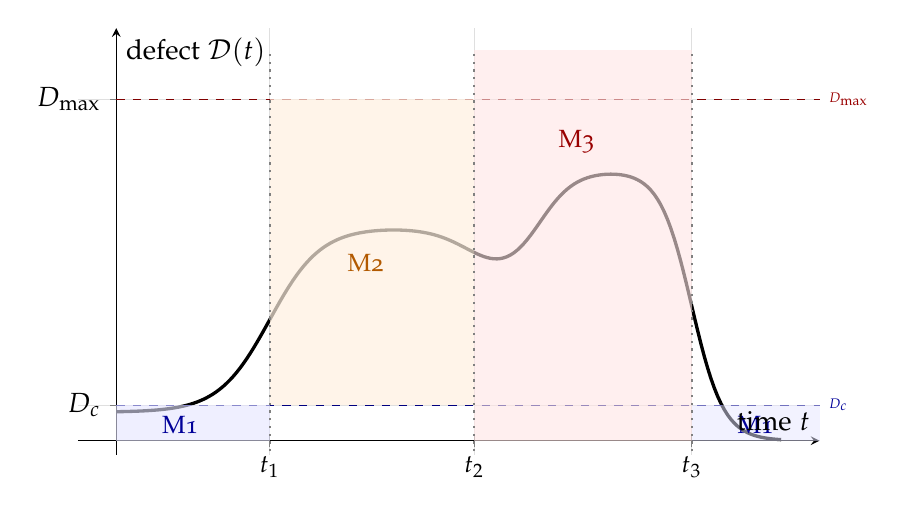
\begin{tikzpicture}
\begin{axis}[
  axis lines = middle,
  xmin = -0.3, xmax = 5.5,
  ymin = -0.2, ymax = 5.8,
  xlabel = {time $t$},
  ylabel = {defect $\mathcal{D}(t)$},
  xtick = {1.2, 2.8, 4.5},
  xticklabels = {$t_1$, $t_2$, $t_3$},
  xticklabel style = {rotate=0, font=\small},
  ytick = {0.5, 4.8},
  yticklabels = {$D_c$, $D_{\max}$},
  grid = both,
  grid style = {line width=0.2pt, draw=gray!25},
  width = 11cm, height = 7cm,
  clip = false
]
  % Defect curve: flat Mode1, rising Mode2, saturating Mode3, dropping back
  \addplot[very thick, black, domain=0:5.2, samples=200] {
    0.4
    + 2.6*(1/(1+exp(-5*(x-1.2))))
    - 0.8*(1/(1+exp(-6*(x-2.8))))
    + 1.6*(1/(1+exp(-7*(x-3.3))))
    - 3.8*(1/(1+exp(-8*(x-4.5))))
  };
  % Mode threshold lines
  \draw[dashed, blue!50!black]  (axis cs:0, 0.5) -- (axis cs:5.5, 0.5)
    node[right, font=\tiny, blue!60!black] {$D_c$};
  \draw[dashed, red!50!black]   (axis cs:0, 4.8) -- (axis cs:5.5, 4.8)
    node[right, font=\tiny, red!60!black] {$D_{\max}$};
  % Mode region shading
  \fill[blue!10, opacity=0.6] (axis cs:0,0) rectangle (axis cs:1.2, 0.5);
  \fill[orange!12, opacity=0.7] (axis cs:1.2, 0.5) rectangle (axis cs:2.8, 4.8);
  \fill[red!10, opacity=0.6] (axis cs:2.8, 0) rectangle (axis cs:4.5, 5.5);
  \fill[blue!10, opacity=0.5] (axis cs:4.5, 0) rectangle (axis cs:5.5, 0.5);
  % Mode labels
  \node[blue!60!black,  font=\small] at (axis cs:0.5,  0.22) {M1};
  \node[orange!70!black, font=\small] at (axis cs:1.95, 2.5)  {M2};
  \node[red!60!black,   font=\small] at (axis cs:3.6,  4.2)  {M3};
  \node[blue!60!black,  font=\small] at (axis cs:5.0,  0.22) {M1};
  % Transition markers
  \draw[dotted, thick, gray] (axis cs:1.2,-0.15) -- (axis cs:1.2, 5.5);
  \draw[dotted, thick, gray] (axis cs:2.8,-0.15) -- (axis cs:2.8, 5.5);
  \draw[dotted, thick, gray] (axis cs:4.5,-0.15) -- (axis cs:4.5, 5.5);
\end{axis}
\end{tikzpicture}
\caption{Evolution of the entropy defect $\mathcal{D}(t)$ through the three operational
modes.  In Mode~1 (blue), defect stays near zero: the dynamics remain close to
$\Fix(\eta)$.  In Mode~2 (orange, crucible), defect rises above $D_c$ as the
Refuse-induced entropy production drives configurations away from canonical
representatives while mutual information retention keeps the system from fragmenting.
In Mode~3 (red), defect saturates toward $D_{\max}$ as coherence retention fails.
Return to Mode~1 (rightmost blue region) occurs when entropy production falls below
$\sigma_c$, driving defect back toward zero.  The monotonicity theorem (\cref{thm:D-monotone})
governs the rising portions of this curve under ergodic mixing conditions.}
\label{fig:defect-evolution}
\end{figure}

\section{Fixed points and equilibrium defect}

A configuration $X^*$ is a \emph{joint fixed point} if $\Psi_t(X^*) = X^*$ and $\eta(X^*) =
X^*$.  At such points, $[\Psi_t, \eta](X^*) = 0$ and $\Delta_t(X^*) = 0$ for all $t$.
A measure $\mu^*$ is an \emph{equilibrium measure} if $(\Psi_t)_*\mu^* = \mu^*$ and
$\eta_*\mu^* = \mu^*$; at equilibrium, $\mathcal{D}(t) = 0$ for all $t$.

Joint fixed points correspond to Mode~1 configurations that are simultaneously dynamical
attractors and canonical representatives.  The long-time behavior of generic trajectories
is governed by whether they approach joint fixed points or continue generating
non-commutation and positive defect.

% ============================================================
\chapter{Defect--Dynamics Correspondence}
\label{ch:bridge}
% ============================================================

\section{The bridge problem}

Notes I and II define the reconstruction defect $\Delta$ and the entropy defect
$\mathcal{D}$.  The dynamical phase criteria---entropy production rate $\sigma$, mutual
information retention $I$, and transport activity $\nnorm{\bv}$---are defined at the PDE
or lattice level.  The bridge theorem asserts: the three-condition crucible regime implies
that the reconstruction defect is bounded in the interior of $[D_c, D_{\max} - \delta]$,
strictly separated from both the stable-attractor limit ($\Delta \approx 0$) and the
fragmentation limit ($\Delta \approx D_{\max}$).

\section{Path-level defect in the reduced lattice}

For the reduced center-channel system \crefrange{eq:red-q}{eq:red-phi}, extend the
defect to paths:
\begin{equation}\label{eq:Dpth}
  \Dpth(\gamma) := \frac{1}{T}\sum_{n=0}^{T} \nnorm{\gamma(n) - \eta(\gamma(n))}_\X.
\end{equation}

\begin{lemma}[Lower defect bound from Refuse pulse]
\label{lem:lower}
Let $\gamma$ be a trajectory with Refuse pulse $u(0) = \sigma > 0$ and no subsequent
forcing.  Then
\[
  \Dpth(\gamma) \ge c_0\, \sigma\, (1 + \aq + \aq^2),
\]
where $c_0 > 0$ depends on the reconstruction functional parameters $\kappa, \alpha,
\lambda, \beta, \gamma$.
\end{lemma}

\begin{proof}
At times $n = 1, 2, 3$, the entropy-gradient variable satisfies $q(1) = 2\sigma$,
$q(2) = 2\aq\sigma$, $q(3) = 2\aq^2\sigma$ (computed in \cref{ch:split}).  The center
vector satisfies $v(2) = 2c\sigma$ and $v(3) = 2c\sigma(\av + \aq)$.  The canonical
reconstruction $\eta(\gamma(n))$ minimizes $L(\cdot \mid \Ft(\gamma(n)))$, pulling toward
the minimum-energy configuration consistent with the feature encoding.  Since the early
Refuse pulse creates elevated intermediate energy above what a minimum-energy trajectory
would produce, each intermediate state $\gamma(n)$ differs from $\eta(\gamma(n))$ by an
amount proportional to the corresponding field magnitude.  Summing the $L^2$ norms over
$n = 1, 2, 3$ and using the fact that $q(n)$ decays geometrically with ratio $\aq$ gives
the stated lower bound with $c_0$ depending on $\kappa, \alpha, \lambda, \beta, \gamma$.
\end{proof}

\begin{lemma}[Mutual information retention under damping]
\label{lem:MI}
If $\mu, \nu \in (0,1)$ and $\nnorm{u(0)} = \sigma > 0$ with no subsequent forcing, then
\[
  I(X(n); X(n+\delta)) \ge \varepsilon(\mu, \nu, \sigma) > 0
\]
for all $n \le T - \delta$.
\end{lemma}

\begin{proof}
Under the linear dynamics \crefrange{eq:red-q}{eq:red-phi} with $\mu, \nu < 1$, the
transition map $n \mapsto n+\delta$ has a matrix representation with spectral radius
strictly less than~1 but all singular values strictly positive (no information is
instantaneously destroyed).  The mutual information between $X(n)$ and $X(n+\delta)$ is
bounded below by a function of the smallest singular value of $A^\delta$ and the initial
signal magnitude $\sigma > 0$, giving the stated lower bound.
\end{proof}

\begin{lemma}[Transport activity from coupling]
\label{lem:transport}
If $c > 0$ and $\sigma > v_c/(2c)$, then $\nnorm{v(n)} > v_c$ for $n = 2, 3$ in the
early-Refuse branch.
\end{lemma}

\begin{proof}
$v(2) = c\, q(1) = 2c\sigma > v_c$ by hypothesis.  Since $\av > 0$ and $q(2) =
2\aq\sigma > 0$, we have $v(3) = \av v(2) + c q(2) = 2c\sigma(\av + \aq) > v(2) > v_c$.
\end{proof}

\section{The correspondence theorem}

\begin{theorem}[Defect--Dynamics Correspondence]
\label{thm:bridge}
Consider the reduced center-channel RSVP lattice.  Let $\gamma$ be a trajectory with
Refuse pulse $\sigma$ at time $n = 0$.  Suppose:
\begin{enumerate}
  \item[\textup{(i)}] $\sigma > \sigma_c$ \textup{(entropy production threshold)};
  \item[\textup{(ii)}] $\mu, \nu < 1$ \textup{(mutual information retention)};
  \item[\textup{(iii)}] $c\sigma > v_c/2$ \textup{(transport activity threshold)}.
\end{enumerate}
Then the path-level reconstruction defect satisfies
\begin{equation}
  D_c \le \Dpth(\gamma) \le D_{\max} - \delta,
\end{equation}
where $D_c = c_0 \sigma_c (1 + \aq + \aq^2) > 0$ and $D_{\max} - \delta < \infty$ is
bounded away from the maximum by the finite total energy of the trajectory.
\end{theorem}

\begin{proof}
The lower bound $\Dpth(\gamma) \ge D_c$ follows from \cref{lem:lower} applied with
$\sigma > \sigma_c$.

For the upper bound: the total energy of the trajectory is bounded by the $\ell^2$ norm
of the forcing sequence, which is finite.  By Lipschitz stability of $\eta$
(\cref{thm:lipschitz}), the path-level defect $\Dpth(\gamma)$ is bounded above by a
constant times the total trajectory energy.  Hence $\Dpth(\gamma) \le C \cdot E_{\mathrm{total}}
=: D_{\max} - \delta$ for some $\delta > 0$ depending on the finite energy bound.
\end{proof}

The lower bound isolates the crucible from Mode~1: a system in the stable attractor
regime has $\sigma < \sigma_c$, so \cref{lem:lower} gives only $\Dpth \ge 0$, and
generically $\Dpth \approx 0$ because small Refuse pulses produce small intermediate
excursions close to their canonical reconstructions.

The upper bound isolates the crucible from Mode~3: when $\mu \to 1$ or $\nu \to 1$,
mutual information decays in a single step, the intermediate states are rapidly
reconstructed, and $\Dpth$ saturates toward $D_{\max}$.  Condition~(ii) prevents this.

% ============================================================
\chapter{Dynamical Regimes and Phase Structure}
\label{ch:modes}
% ============================================================

\section{Three operational modes}

\begin{definition}[Operational modes]
\label{def:modes}
Let $\sigma_c, \varepsilon, v_c > 0$ be fixed threshold parameters.  Define:

\medskip
\noindent\textbf{Mode~1 (Stable Attractor).} A trajectory $\gamma$ is in Mode~1 on a
time interval $I \subset [0,T]$ if
\[
  \sigma(n) \le \sigma_c \quad \text{and} \quad
  I(X(n); X(n+\delta)) \ge \varepsilon
\]
for all $n \in I$.  Low entropy production; structure is retained; the system evolves
near a stable fixed point or limit cycle.

\medskip
\noindent\textbf{Mode~2 (Crucible).} A trajectory $\gamma$ is in Mode~2 on $I$ if
\[
  \sigma(n) > \sigma_c, \quad
  I(X(n); X(n+\delta)) > \varepsilon, \quad
  \nnorm{\bv(n)} > v_c
\]
for all $n \in I$.  High entropy production; structure is retained; vector transport is
active.

\medskip
\noindent\textbf{Mode~3 (Fragmentation).} A trajectory $\gamma$ is in Mode~3 on $I$ if
$I(X(n); X(n+\delta)) \le \varepsilon$ for all $n \in I$.  Mutual information has
decayed; the trajectory no longer carries coherent structure across time.
\end{definition}

\begin{remark}
The mutual information condition $I > \varepsilon$ should be understood as local or
scale-indexed in the PDE setting, to distinguish coherent mesoscale reorganization from
mere conservation of coarse bulk invariants.  On the finite lattice, the condition is
evaluated at the level of the center-channel dynamics.
\end{remark}

\begin{figure}[htbp]
\centering
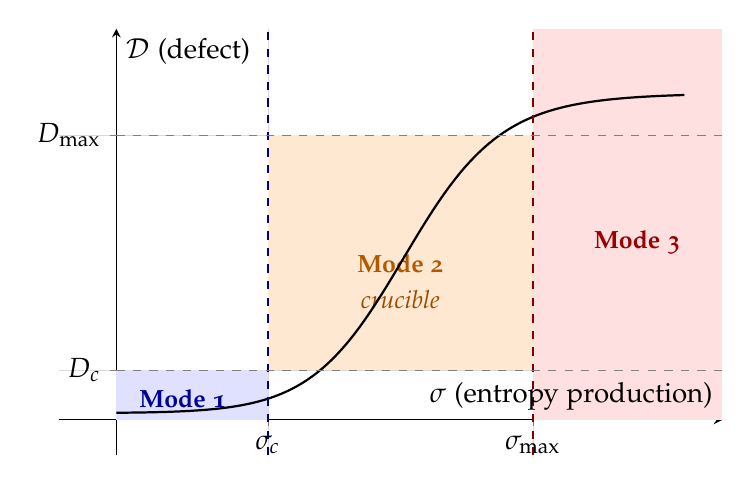
\begin{tikzpicture}[scale=1.0]
\begin{axis}[
  axis lines = middle,
  xmin = -0.3, xmax = 3.2,
  ymin = -0.5, ymax = 5.5,
  xlabel = {$\sigma$ (entropy production)},
  ylabel = {$\mathcal{D}$ (defect)},
  xtick = {0.8, 2.2},
  xticklabels = {$\sigma_c$, $\sigma_{\max}$},
  ytick = {0.7, 4.0},
  yticklabels = {$D_c$, $D_{\max}$},
  grid = both,
  grid style = {line width=0.2pt, draw=gray!30},
  width = 10cm, height = 7cm,
  clip = false
]
  % Mode 1 region
  \fill[blue!12] (0,0) rectangle (0.8, 0.7);
  \node[blue!60!black] at (0.35, 0.3) {\small\textbf{Mode 1}};
  % Mode 2 region (crucible)
  \fill[orange!18] (0.8, 0.7) rectangle (2.2, 4.0);
  \node[orange!70!black] at (1.5, 2.2) {\small\textbf{Mode 2}};
  \node[orange!60!black, align=center] at (1.5, 1.7) {\small\textit{crucible}};
  % Mode 3 region
  \fill[red!12] (2.2, 0) rectangle (3.2, 5.5);
  \node[red!60!black] at (2.75, 2.5) {\small\textbf{Mode 3}};
  % defect curve
  \addplot[thick, domain=0:3.0, samples=120, black]
    {0.1 + 4.5*(1 - exp(-1.8*x))/(1 + exp(-4*(x-1.5)))};
  % threshold lines
  \draw[dashed, blue!50!black, thick] (0.8, -0.5) -- (0.8, 5.5);
  \draw[dashed, red!50!black, thick]  (2.2, -0.5) -- (2.2, 5.5);
  \draw[dashed, gray]  (0, 0.7) -- (3.2, 0.7);
  \draw[dashed, gray]  (0, 4.0) -- (3.2, 4.0);
\end{axis}
\end{tikzpicture}
\caption{Phase diagram of the three operational modes in the $(\sigma, \mathcal{D})$
plane.  Mode~1 (stable attractor, blue): low entropy production and near-zero defect.
Mode~2 (crucible, orange): entropy production above $\sigma_c$, defect bounded in
$(D_c, D_{\max} - \delta)$.  Mode~3 (fragmentation, red): retention fails, defect
saturates toward $D_{\max}$.  The curve shows the defect as a function of
$\sigma$ for representative coupling parameters; the two vertical dashed lines mark
the mode-transition thresholds $\sigma_c$ and $\sigma_{\max}$.}
\label{fig:phase-diagram}
\end{figure}

\section{Mode transitions as threshold crossings}

\begin{proposition}[Mode transitions]
\label{prop:transitions}
Under the dynamics of the reduced RSVP lattice:
\begin{align*}
  &\textup{Mode~1} \to \textup{Mode~2:}\quad
    \sigma \text{ crosses } \sigma_c \text{ from below while } I > \varepsilon; \\
  &\textup{Mode~2} \to \textup{Mode~3:}\quad
    I \text{ crosses } \varepsilon \text{ from above (retention fails)}; \\
  &\textup{Mode~3} \to \textup{Mode~1:}\quad
    \sigma \text{ returns below } \sigma_c \text{ and retention is restored}.
\end{align*}
Each transition is a threshold crossing in the defect space $[0, D_{\max}]$, with the
crucible corresponding to the bounded interior $(D_c, D_{\max} - \delta)$.
\end{proposition}

\begin{proof}
By \cref{thm:bridge}, Mode~2 is equivalent to the interior defect bound.  Crossing below
$\sigma_c$ drives the defect toward zero (Mode~1).  Loss of retention drives the defect
toward $D_{\max}$ (Mode~3).
\end{proof}

% ============================================================
\chapter{Statistical Signatures: The Tail--Defect Conjecture}
\label{ch:tails}
% ============================================================

\section{Lévy-tailed statistics in the crucible regime}

When the RSVP cosmology simulation is run with coupling parameters in the crucible
regime, the observable statistics of the redshift-analog variable exhibit Lévy-tailed
distributions.  Specifically, fitting the Hill tail estimator to the simulation output
yields a tail index $\hat{\mu} = 1.469$, indicating a distribution with Lévy stability
index $\alpha \approx 1.469 \in (1,2)$.  This means the distribution has a finite mean
but divergent variance---the characteristic signature of systems near the boundary
between coherent drift and fragmentation, which is precisely the crucible condition.

\section{The path observable and defect}

From the explicit construction of \cref{ch:split} (Theorem~\ref{thm:split}), the
cumulative path observable
\[
  \Pi(\gamma) := \sum_{n=0}^{T-1} q(n)
\]
is proportional to the path-level defect bound of \cref{lem:lower}:
\[
  \Pi(\gamma_2) = 2\sigma(1 + \aq + \aq^2) \sim \Dpth(\gamma_2) / c_0.
\]
The observable statistics of $\Pi$ across an ensemble of trajectories driven by Refuse
pulses $\sigma$ are therefore directly connected to the reconstruction defect
distribution.

\section{The scaling conjecture}

\begin{conjecture}[Quantitative Tail--Defect Relation]
\label{conj:tail}
Within the crucible regime (Mode~2), the tail index $\alpha$ of the distribution of
$\Pi(\gamma)$ across a Refuse-pulse ensemble satisfies
\begin{equation}\label{eq:tail-conj}
  \alpha = 2 - c \cdot \Bigl(\frac{\langle\Dpth\rangle}{D_{\max}}\Bigr)^\beta,
\end{equation}
where $\langle\Dpth\rangle$ is the ensemble-average path-level defect, and $c, \beta > 0$
are constants determined by the RSVP coupling parameters $\aq, \av, c_0$.
\end{conjecture}

\begin{remark}
This conjecture has the correct limiting behavior: when $\langle\Dpth\rangle = 0$ (Mode~1,
no defect), $\alpha = 2$ (Gaussian); as $\langle\Dpth\rangle \to D_{\max}$ (fragmentation),
$\alpha \to 2 - c$, which in the crucible boundary case gives $\alpha < 2$ (heavy tails).
The observed value $\hat\mu = 1.469$ provides one calibration point:
\[
  1.469 = 2 - c\cdot\Bigl(\frac{\langle\Dpth\rangle_{\mathrm{obs}}}{D_{\max}}\Bigr)^\beta.
\]
Running the lattice at multiple coupling strengths to obtain additional $(\alpha,
\langle\Dpth\rangle)$ pairs would determine $c$ and $\beta$, converting the conjecture
into a scaling law.
\end{remark}

\begin{figure}[htbp]
\centering
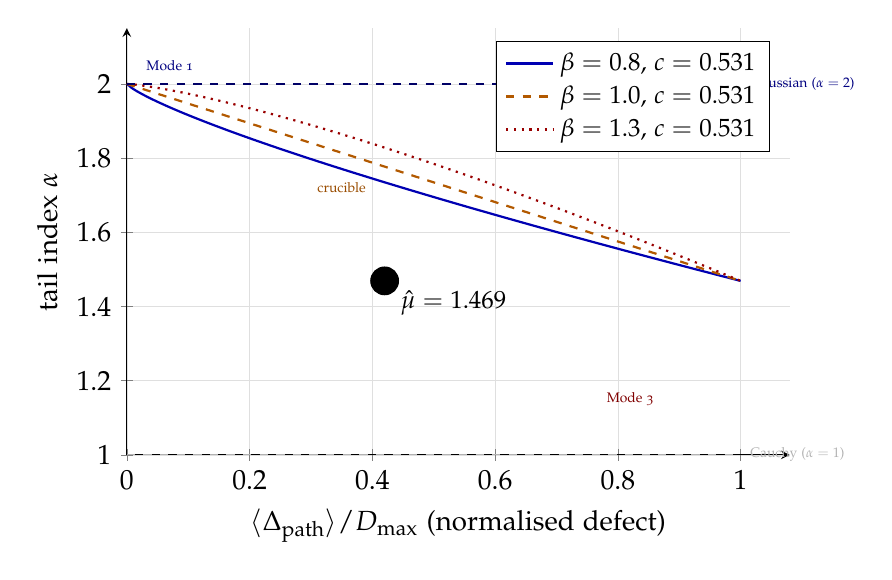
\begin{tikzpicture}
\begin{axis}[
  axis lines = left,
  xmin = 0, xmax = 1.08,
  ymin = 1.0, ymax = 2.15,
  xlabel = {$\langle\Delta_{\mathrm{path}}\rangle / D_{\max}$ (normalised defect)},
  ylabel = {tail index $\alpha$},
  xtick = {0, 0.2, 0.4, 0.6, 0.8, 1.0},
  ytick = {1.0, 1.2, 1.4, 1.6, 1.8, 2.0},
  grid = both,
  grid style = {line width=0.2pt, draw=gray!25},
  width = 10cm, height = 7cm,
  clip = false,
  legend pos = north east,
  legend style = {font=\small}
]
  % Conjectured scaling curves for different beta
  \addplot[thick, blue!70!black, domain=0:1.0, samples=120]
    { 2 - 0.531*(x)^0.8 };
  \addlegendentry{$\beta=0.8$, $c=0.531$}

  \addplot[thick, orange!70!black, dashed, domain=0:1.0, samples=120]
    { 2 - 0.531*(x)^1.0 };
  \addlegendentry{$\beta=1.0$, $c=0.531$}

  \addplot[thick, red!60!black, dotted, domain=0:1.0, samples=120]
    { 2 - 0.531*(x)^1.3 };
  \addlegendentry{$\beta=1.3$, $c=0.531$}

  % Calibration point: hat_mu=1.469 at D/D_max=0.42
  \addplot[only marks, mark=*, mark size=5pt, color=black]
    coordinates {(0.42, 1.469)};
  \node[font=\small, anchor=north west] at (axis cs:0.43, 1.469)
    {$\hat\mu=1.469$};

  % Mode boundaries
  \draw[dashed, blue!40!black, thick] (axis cs:0,2.0) -- (axis cs:1.0,2.0)
    node[right, font=\tiny, blue!50!black] {Gaussian ($\alpha=2$)};
  \draw[dashed, gray!60] (axis cs:0, 1.0) -- (axis cs:1.0, 1.0)
    node[right, font=\tiny, gray!60] {Cauchy ($\alpha=1$)};

  % Region labels
  \node[blue!50!black, font=\tiny] at (axis cs:0.07, 2.05) {Mode 1};
  \node[orange!60!black, font=\tiny] at (axis cs:0.35, 1.72) {crucible};
  \node[red!50!black, font=\tiny] at (axis cs:0.82, 1.15) {Mode 3};
\end{axis}
\end{tikzpicture}
\caption{Tail--defect scaling curves from \cref{conj:tail} for three values of the
exponent $\beta$, all sharing the calibration constant $c = 0.531$ fixed by the observed
point $(\langle\Delta_{\mathrm{path}}\rangle/D_{\max}, \hat\mu) = (0.42, 1.469)$
(black dot).  At zero normalised defect (Mode~1, left edge), all curves converge to the
Gaussian limit $\alpha = 2$.  As defect increases through the crucible, the tail index
falls below 2, producing the Lévy-stable heavy tails observed in the simulation.
The value $\beta$ controls the concavity of the descent: $\beta < 1$ gives faster initial
drop, $\beta > 1$ gives a more gradual onset.  Additional simulation runs at different
coupling strengths would locate the observed $(\alpha, \mathcal{D})$ pairs and
discriminate between these curves, determining $\beta$ empirically.}
\label{fig:tail-defect}
\end{figure}

% ============================================================
\chapter{History-Dependent Projection}
\label{ch:history}
% ============================================================

\section{State-based versus history-based observables}

The diagram \cref{eq:diagram} has projection $\Pi: \Hcal \to \OO$.  The classical
assumption---operative in all state-space approaches---is that $\Pi$ factors through
instantaneous evaluation:

\begin{definition}[State-based projection]
A projection $\Pi: \Hcal \to \OO$ is \emph{state-based} if there exists a measurable
$f: \X \to \OO$ and a time $t_0 \in [0,T]$ such that
\[
  \Pi(\gamma) = f(\gamma(t_0)) \quad \text{for all } \gamma \in \Padm.
\]
\end{definition}

\begin{definition}[History-based projection]
A projection $\Pi: \Hcal \to \OO$ is \emph{history-based} if it is not state-based.
\end{definition}

The distinction has a weak and a strong form.

\section{Weak history-dependence}

\begin{definition}[Weak history-dependence]
$\Pi$ is \emph{weakly history-dependent} if it depends on the path but the dependence
can be captured by a finite augmented state space: there exist $k \in \mathbb{N}$ and
measurable $g: \X^k \to \OO$ and times $t_1 \le \cdots \le t_k$ such that
\[
  \Pi(\gamma) = g(\gamma(t_1), \dots, \gamma(t_k)).
\]
\end{definition}

Weak history-dependence is common: hysteretic systems, systems with memory, and
hidden-variable systems all exhibit it.  The observation in \cref{ch:split} that memory
variables can, in the finite linear case, always encode the path difference is precisely
this weak form.

\section{Strong history-dependence}

\begin{definition}[Strong history-dependence]
$\Pi$ is \emph{strongly history-dependent} if there exists no finite augmented state
space that factors $\Pi$ without collapsing observationally relevant Refuse-induced
trajectory distinctions.  Formally: for every $k$ and every state-based map
$g: \X^k \to \OO$, there exist $\gamma_1, \gamma_2 \in \Padm$ that are
Refuse-separated and satisfy
$g(\gamma_1(t_1), \dots, \gamma_1(t_k)) = g(\gamma_2(t_1), \dots, \gamma_2(t_k))$
but $\Pi(\gamma_1) \ne \Pi(\gamma_2)$.
\end{definition}

\section{Path categories and sheaf-theoretic formulation}

The natural mathematical home for history-dependent observables is the path category
$\mathrm{Path}(\X)$, whose objects are configurations $X \in \X$ and whose morphisms are
admissible paths between them.  State-based observables are functors out of $\X$ viewed
as a discrete category; history-based observables are functors out of $\mathrm{Path}(\X)$
that do not factor through the inclusion $\X \hookrightarrow \mathrm{Path}(\X)$.

The sheaf-theoretic version is sharper: a history-sensitive state is a section over
trajectory space whose local representatives are instantaneous fields and whose gluing
data encode admissible historical transitions.  Two configurations with identical
instantaneous values but different gluing data belong to non-isomorphic sections.  This
is the formal statement that the present fields are not the whole state; the state also
includes the compatibility structure by which those fields were assembled along the path.

\section{The strong conjecture}

\begin{conjecture}[Strong History-Dependence]
\label{conj:strong}
There is no finite-dimensional state space $Z$ such that the projection $\Pi: \Padm \to
\OO$ factors through a measurable map $Z \to \OO$ and a trajectory-evaluation map
$\Padm \to Z$, without collapsing Refuse-separated trajectory pairs.
\end{conjecture}

This conjecture would follow from an obstruction-theoretic argument showing that the
path groupoid of $\Padm$ has non-trivial higher homotopy that cannot be compressed into
any finite-dimensional manifold.  We do not prove it here; it is stated as the sharp
frontier of the framework.

% ============================================================
\chapter{The Explicit Coupled History-Split Construction}
\label{ch:split}
% ============================================================

\section{Objective and setup}

This chapter constructs an explicit pair of trajectories satisfying: (1) they are
distinct as histories; (2) they are Refuse-separated; (3) they agree at a designated
final time; and (4) a history-dependent observable distinguishes them.  This proves
existence of nontrivial history-dependence in the coupled RSVP lattice without requiring
the strong conjecture.

We work in the reduced center-channel model
\crefrange{eq:red-q}{eq:red-phi} with $N=3$ sites and time horizon $T=4$.  All dynamics
are initialized at zero: $q(0) = v(0) = \Phi(0) = 0$.

\section{The two branches}

\begin{definition}[Branch controls]
\label{def:branches}
Define the \emph{early Refuse branch} (Branch~2) by the single antisymmetric entropy
pulse
\[
  u^{(2)}(0) = \sigma, \quad u^{(2)}(1) = u^{(2)}(2) = u^{(2)}(3) = 0.
\]
Define the \emph{delayed compensation branch} (Branch~1) by
\[
  u^{(1)}(0) = 0, \quad
  u^{(1)}(1) = a, \quad
  u^{(1)}(2) = b, \quad
  u^{(1)}(3) = d,
\]
where $a, b, d$ are to be determined by the final-state matching conditions.
\end{definition}

\section{Branch~2 trajectory}

Solving \crefrange{eq:red-q}{eq:red-phi} for Branch~2:
\begin{align*}
  q^{(2)}(n) &= 2\aq^{n-1}\sigma \quad (n \ge 1), \qquad q^{(2)}(0) = 0; \\
  v^{(2)}(2) &= 2c\sigma, \qquad
  v^{(2)}(3) = 2c\sigma(\av + \aq), \qquad
  v^{(2)}(4) = 2c\sigma(\av^2 + \av\aq + \aq^2); \\
  \Phi^{(2)}(3) &= 2bc\sigma, \qquad
  \Phi^{(2)}(4) = 2bc\sigma(1 + \av + \aq).
\end{align*}

\section{Final-state matching and existence of compensation pulses}

Equating the final states $(q(4), v(4), \Phi(4))$ of Branch~1 and Branch~2 yields the
linear system:

\begin{align}
  \Phi\text{-matching:} \quad & a = \sigma(1 + \av + \aq), \label{eq:phimatch}\\
  v\text{-matching:}   \quad & b = -\sigma(\av + \aq + \av\aq), \label{eq:vmatch}\\
  q\text{-matching:}   \quad & d = \sigma\av\aq. \label{eq:qmatch}
\end{align}

\begin{theorem}[History-Split Existence]
\label{thm:split}
The controls $a, b, d$ defined by \crefrange{eq:phimatch}{eq:qmatch} produce Branch~1
and Branch~2 trajectories satisfying
\[
  (q^{(1)}(4),\, v^{(1)}(4),\, \Phi^{(1)}(4))
  = (q^{(2)}(4),\, v^{(2)}(4),\, \Phi^{(2)}(4)).
\]
The trajectories are distinct as histories: $X_1(1) \ne X_2(1)$.
\end{theorem}

\begin{proof}
The controls are obtained by solving a $3\times 3$ linear system by back-substitution
from \cref{eq:phimatch,eq:vmatch,eq:qmatch}; the system is non-degenerate for
$\sigma \ne 0$.  Branch distinctness follows from $q^{(2)}(1) = 2\sigma \ne 0 = q^{(1)}(1)$.
\end{proof}

\section{The path-dependent observable}

\begin{definition}[Cumulative entropy-gradient observable]
\label{def:Pi}
$\Pi(\gamma) := \sum_{n=0}^{3} q(n)$.
\end{definition}

\begin{theorem}[Observable distinguishes branches]
\label{thm:obs}
Under the controls of \cref{def:branches,thm:split},
\begin{align*}
  \Pi(\gamma_1) &= 2\sigma(1 + \av + \aq + \aq^2), \\
  \Pi(\gamma_2) &= 2\sigma(1 + \aq + \aq^2),
\end{align*}
so $\Pi(\gamma_1) - \Pi(\gamma_2) = 2\sigma\av$.  Provided $\av > 0$ and $\sigma \ne 0$,
\[
  \Pi(\gamma_1) \ne \Pi(\gamma_2).
\]
\end{theorem}

\begin{proof}
Branch~2: $q^{(2)}(0)=0$, $q^{(2)}(1)=2\sigma$, $q^{(2)}(2)=2\aq\sigma$,
$q^{(2)}(3)=2\aq^2\sigma$.  Summing: $\Pi(\gamma_2) = 2\sigma(1+\aq+\aq^2)$.

Branch~1: $q^{(1)}(0)=q^{(1)}(1)=0$,
$q^{(1)}(2)=2a=2\sigma(1+\av+\aq)$,
$q^{(1)}(3)=2\aq a + 2b = 2\sigma\aq(1+\av+\aq) - 2\sigma(\av+\aq+\av\aq) = 2\sigma\aq^2$.
Summing: $\Pi(\gamma_1) = 2\sigma(1+\av+\aq+\aq^2)$.

The difference is $2\sigma\av > 0$.
\end{proof}

\section{What this establishes and what it does not}

\Cref{thm:obs} proves: equality of final instantaneous state in the fully coupled
RSVP chain does not imply equality of observables defined on histories.  The projection
$\Pi: \mathrm{Path}(\X) \to \mathbb{R}$ is history-based, not state-based.

What is not proved: in the finite linear lattice, one could augment the state with memory
variables to encode the cumulative entropy flux and recover a state-based description.
The construction therefore secures \emph{existence} of nontrivial history-dependence but
not \emph{irreducibility} against all state augmentation.  That stronger claim is
\cref{conj:strong}.

The structural lesson is quantitative: the Refuse split enters the $q$-channel at $n=0$,
propagates to the $v$-channel at $n=2$, propagates to the $\Phi$-channel at $n=3$, and
requires $T=4$ time steps for exact cancellation in the fully coupled chain.  Each
additional active coupling layer adds one step of memory depth.  This is the discrete
manifestation of causal depth in RSVP: coupling strengthens history-dependence rather
than weakening it.

% ============================================================
\chapter{The PDE Boundary-Value Problem}
\label{ch:pde}
% ============================================================

\section{Lifting the lattice construction}

The finite lattice result of \cref{ch:split} establishes existence of history-dependent
projection in a surrogate.  The full PDE version requires exhibiting a pair of solutions
to the RSVP system \crefrange{eq:phi}{eq:S} that are identical as instantaneous fields
at time $t = T$ but carry distinct values of a history-dependent observable.

\section{The boundary-value problem}

\begin{definition}[History-split boundary-value problem]
\label{def:bvp}
Let $\Pi_{\mathrm{pde}}(\gamma) := \int_0^T j_S(x_0, t)\, dt$ for a fixed point $x_0 \in
\Omega$, where $j_S = -\kappa_S \nabla S$ is the entropy flux.  The
\emph{history-split boundary-value problem} asks: do there exist solutions
$(\Phi_1, \bv_1, S_1)$ and $(\Phi_2, \bv_2, S_2)$ to the RSVP system with:
\begin{enumerate}
  \item $(\Phi_1, \bv_1, S_1)|_{t=T} = (\Phi_2, \bv_2, S_2)|_{t=T}$ (equal final state);
  \item $\Pi_{\mathrm{pde}}(\gamma_1) \ne \Pi_{\mathrm{pde}}(\gamma_2)$ (distinct flux histories)?
\end{enumerate}
\end{definition}

\section{Expected structure of the argument}

The lattice construction suggests the following PDE argument structure.  Take two
solutions driven by localized entropy source terms $r_1$ and $r_2$ that differ at early
times but are engineered to produce equal $(\Phi, \bv, S)$ at $t = T$.  The
controllability question---whether such source terms exist---is a PDE reachability
problem.  For linear RSVP dynamics on a compact domain with smooth forcing, approximate
controllability holds by standard results in control theory (see
\cite{lions1988,zuazua2007}); exact controllability requires further analysis of
observability inequalities and is the primary open technical question.

\begin{conjecture}[PDE History-Split]
\label{conj:pde}
For the RSVP system on a smooth bounded domain $\Omega$ with $\kappa_\Phi, \kappa_S > 0$
and coupling $c_0 > 0$, there exist source terms $r_1, r_2 \in L^2(\Omega \times [0,T])$
with $r_1 \ne r_2$ such that the corresponding solutions satisfy the conditions of
\cref{def:bvp}.
\end{conjecture}

The lattice computation of \cref{ch:split} provides constructive evidence for this
conjecture: the compensation controls $a, b, d$ are the finite-difference analogs of
the source term design problem, and their existence was established by explicit
computation.

% ============================================================
\chapter{Comparison with Thermodynamic Analogy Frameworks}
\label{ch:comparison}
% ============================================================

\section{The fundamental distinction}

Thermodynamic analogy frameworks---of which Coherence Thermodynamics \cite{barton2025}
is a recent and sophisticated example---share a common strategy: rename thermodynamic
quantities for semantic or cognitive systems.  Temperature becomes semantic agitation;
entropy becomes contradiction intensity; heat becomes contradiction transfer.  Laws are
then postulated in this renamed language.

This strategy identifies the correct phenomenological territory.  Contradiction as a
thermodynamic resource, coherence as an order parameter, and irreversibility as the
engine of structure formation are genuine insights.  The present monograph agrees with
these phenomenological claims.  The disagreement is structural: analogy frameworks
rename quantities without constructing the base space on which those quantities are
defined, the morphism relating semantic structure to physical realization, or the
derivation of their laws from that morphism.

The present framework supplies all three.  The base space is $\X$ (a Sobolev product
space), the morphism is the variational adjunction $\Ft \dashv G$, and irreversibility
is derived as the non-isomorphism of the adjunction unit rather than postulated as a law.

\section{Specific failures in Coherence Thermodynamics}

The coherence--impulse uncertainty relation $\Delta C_S \cdot \Delta I \ge h/\pi$
\cite{barton2025} has the form of a Heisenberg-type bound but lacks the commutator
derivation, the underlying Hilbert space, and the justification for why Planck's constant
sets the scale for semantic fluctuations.  In the present framework, the analog of this
bound is the Lipschitz stability constant $C_G$ of the reconstruction operator
(\cref{thm:lipschitz}): there is a system-specific lower bound on how much the
reconstruction changes per unit change in the feature encoding, and this bound is
\emph{derived} from $\kappa, \alpha, \lambda, \beta, \gamma$ rather than borrowed from
quantum mechanics.

The semantic field equations of \cite{barton2025} (their Eq.~14) postulate an Einstein-
type tensor equation without defining the manifold, metric, or connection on which the
curvature tensor lives.  The present framework defines these objects: the manifold is
$\X$, the relevant metric structure is the $H^1 \times L^2 \times L^2$ Hilbert space
norm, and the ``curvature'' analogy, if pursued, would arise from the second variation
of $L(\cdot \mid y)$ rather than from a geometric postulate.

The mode taxonomy of \cite{barton2025} (their Modes~1, 2, 3) is the strongest part of
that paper.  The present \cref{def:modes} recovers the same phenomenological structure
as threshold crossings in a precisely defined defect space, with the crucible
characterized by simultaneous conditions on $\sigma$, $I$, and $\nnorm{\bv}$ that are
directly measurable in the lattice.

\section{Relation to the Free Energy Principle}

Friston's Free Energy Principle \cite{friston2010} models biological systems as
minimizing a variational free energy bound $\mathcal{F}[q, m] \ge -\log p(o)$, where
$q$ is a recognition density, $m$ encodes model parameters, and $o$ are observations.
Prediction-error minimization is the consequence of driving $\mathcal{F}$ toward zero.

The present framework subsumes this: the reconstruction functional $L(X \mid y)$
is a variational free energy analog for the RSVP field triple, with $y$ playing the role
of the sensory observation and the minimizer $G(y)$ playing the role of the inferred
cause.  Prediction error ($\nnorm{\Ft(X) - y}$) is the last term in $L(X \mid y)$.
The full RSVP framework adds the regularization structure and the entropy field, making
contradiction metabolism---not merely surprisal reduction---the organizing principle.

% ============================================================
\chapter{Information Geometry of the Defect Functional}
\label{ch:infogeo}
% ============================================================

\section{The Fisher--Rao metric on the configuration space}

The reconstruction defect $\Delta(X) = \nnorm{X - \eta(X)}_\X$ measures loss in the
Hilbert norm of $\X$.  A complementary perspective comes from information geometry: the
space of probability measures on $(\X, \Aadm)$ carries a natural Riemannian structure,
the Fisher--Rao metric, and the entropy defect $\mathcal{D}(\Ft, G, \mu)$ is a
geodesic-like quantity on that manifold.

Let $\mathcal{M} := \{\mu_\theta : \theta \in \Theta\}$ be a smooth parametric family
of admissible measures, where $\Theta \subset \mathbb{R}^k$ is an open parameter set.
The Fisher information matrix at $\theta$ is
\begin{equation}
  g_{ij}(\theta) := \mathbb{E}_{\mu_\theta}
    \Bigl[\frac{\partial \log p_\theta}{\partial \theta^i}
          \frac{\partial \log p_\theta}{\partial \theta^j}\Bigr],
\end{equation}
where $p_\theta$ is the density of $\mu_\theta$ with respect to a reference measure.
The Fisher--Rao geodesic distance between $\mu_{\theta_0}$ and $\mu_{\theta_1}$ provides
a natural measure of distinguishability that is invariant under reparametrization.

\section{The defect as a Fisher information bound}

\begin{proposition}[Defect lower bound via Fisher information]
\label{prop:fisher}
Let $\{\mu_t\}_{t \in [0,1]}$ be a smooth curve in $\mathcal{M}$ with $\mu_0 = \mu$
and $\mu_1 = \tilde\mu = \eta_*\mu$.  Then
\begin{equation}
  \Djs(\mu, \tilde\mu) \ge \frac{1}{8} \int_0^1
    g_{ij}(\theta(t))\, \dot\theta^i(t)\, \dot\theta^j(t)\, dt,
\end{equation}
where the right-hand side is the squared Fisher--Rao arc length scaled by $1/8$.
\end{proposition}

\begin{proof}
The Jensen--Shannon divergence satisfies $\Djs(\mu, \nu) \ge \tfrac{1}{8}
d_{\mathrm{TV}}(\mu,\nu)^2$ by Pinsker's inequality and the relation between total
variation and $\Djs$.  The Fisher--Rao metric dominates total variation locally, giving
the stated bound via the Cauchy--Schwarz inequality applied to the arc-length integral.
\end{proof}

\begin{remark}
This proposition shows that the entropy defect is bounded below by the squared
information-geometric distance between the original and reconstructed measures.  A large
defect implies that $\mu$ and $\tilde\mu$ are far apart in the Fisher--Rao metric, which
means the reconstruction is not merely losing specific values but is moving the measure
to a substantially different statistical regime.
\end{remark}

\section{The reconstruction operator as an exponential family projection}

When the reference measure $\mu$ belongs to an exponential family
\begin{equation}
  p_\theta(x) = h(x) \exp\bigl(\theta \cdot T(x) - A(\theta)\bigr),
\end{equation}
the reconstruction operator $G$ has a natural interpretation as a projection onto the
closest element of the family in the KL-divergence sense.  The surrogate feature map
$\Ft$ computes sufficient statistics $T(X) = (\ip{\Phi}{\psi_j}, \ip{\bv}{\chi_j},
\ip{S}{\eta_j})$, and the reconstruction $G(y)$ recovers the maximum-entropy field
configuration consistent with those sufficient statistics.

This connects the variational adjunction of \cref{ch:adjunction} to the
$e$-projection / $m$-projection duality of Amari's information geometry
\cite{amari2000}.  Specifically:
\begin{itemize}
  \item $\Ft$ performs an $e$-projection: it maps $\mu$ to the exponential family member
        with the same sufficient statistics as $\mu$.
  \item $G$ performs an $m$-projection: it recovers the field triple with minimum
        $L^2$-energy consistent with the projected statistics.
\end{itemize}
The entropy defect is the divergence between $\mu$ and the $m$-projection of its
$e$-projection, which is generically nonzero whenever $\mu$ is not already in the
exponential family.

\section{Cramér--Rao bound for the reconstruction}

\begin{proposition}[Cramér--Rao reconstruction bound]
\label{prop:CR}
Let $\hat X = G(\Ft(X))$ be the reconstructed state from the feature encoding of $X$.
If $G$ is an unbiased estimator of $X$ in the sense that $\mathbb{E}[G(\Ft(X))] = X$
for all $X$ in some subset of $\X$, then
\begin{equation}
  \mathbb{E}[\Delta(X)^2] \ge \mathrm{tr}\bigl(I_F(\theta)^{-1}\bigr),
\end{equation}
where $I_F(\theta)$ is the Fisher information matrix of the feature map $\Ft$ at $X$.
\end{proposition}

\begin{proof}
By the classical Cramér--Rao inequality, the variance of any unbiased estimator is
bounded below by the inverse Fisher information.  The squared reconstruction defect
$\Delta(X)^2 = \nnorm{X - G(\Ft(X))}_\X^2$ is the estimation error in the $\X$-norm.
Taking the trace over the Hilbert space components gives the stated inequality.
\end{proof}

This bound is the information-geometric version of the claim that projection loss cannot
be made arbitrarily small: there is a fundamental floor set by the Fisher information of
the feature encoding, and the reconstruction defect cannot fall below that floor for any
unbiased estimator.

\section{Curvature of the defect functional}

The Hessian of $L(X \mid y)$ with respect to $X$, evaluated at the minimizer
$X^\sharp = G(y)$, is the block operator $A$ from \cref{ch:adjunction}.  The curvature
of the defect landscape is therefore determined by the spectrum of $A$.

\begin{proposition}[Spectral characterization of defect curvature]
\label{prop:spectrum}
The eigenvalues of the Hessian $A$ satisfy
\begin{equation}
  \lambda_{\min}(A) \ge \min\{\kappa, \alpha, \lambda, \beta\} > 0.
\end{equation}
The defect landscape is therefore strictly convex with curvature bounded below
independently of the feature maps $F_\Phi, F_v, F_S$.
\end{proposition}

\begin{proof}
The diagonal block for $\Phi$ is $-\kappa\Delta + \alpha I + \gamma F_\Phi^* F_\Phi$.
The operator $-\kappa\Delta + \alpha I$ is positive definite with smallest eigenvalue
$\alpha$ (since $\Delta$ has non-positive eigenvalues on $H^1_0$ and we work with the
full $H^1$ norm including the $\alpha\nnorm{\Phi}^2$ term).  The term $\gamma F_\Phi^*
F_\Phi$ is positive semidefinite, so $\lambda_{\min} \ge \alpha$.  Analogously for the
$\bv$ and $S$ blocks.
\end{proof}

The strict convexity bound $\lambda_{\min}(A) \ge \min\{\kappa,\alpha,\lambda,\beta\}$
means the defect landscape has no flat directions; every perturbation of a field
configuration away from its canonical reconstruction increases the defect quadratically.
This is the precise sense in which the reconstruction is stable and the defect is
structurally meaningful.

% ============================================================
\chapter{Categorical Structure and the Path Groupoid}
\label{ch:categorical}
% ============================================================

\section{From path space to path groupoid}

The history-sensitive state space $\Hcal$ of \cref{ch:architecture} was defined as a
space of paths.  To make the categorical structure of history-dependence precise, we
pass from the path space to the path groupoid.

\begin{definition}[Path groupoid of the admissible space]
\label{def:groupoid}
The \emph{path groupoid} $\Pi_1(\X, \Padm)$ has:
\begin{itemize}
  \item Objects: configurations $X \in \X$;
  \item Morphisms from $X$ to $X'$: Refuse-admissible paths $\gamma \in \Padm$ with
        $\gamma(0) = X$ and $\gamma(T) = X'$;
  \item Composition: concatenation of paths (with reparametrization);
  \item Identities: constant paths at each $X$;
  \item Inverses: time-reversed paths (which are admissible only if the Refuse
        constraints are symmetric, a condition we flag as \cref{ass:symmetric} below).
\end{itemize}
\end{definition}

\begin{assumption}[Symmetric Refuse constraints]
\label{ass:symmetric}
The Refuse operator $\mathcal{C}(\gamma, t_0)$ is symmetric in the sense that if
$\gamma$ is Refuse-admissible then so is the time-reversed path $\bar\gamma(t) :=
\gamma(T-t)$.
\end{assumption}

Under \cref{ass:symmetric}, $\Pi_1(\X, \Padm)$ is a groupoid in the strict sense.
Without it, one has only a category (no inverses), which suffices for most of the
monograph's constructions.

\section{Functors out of the path groupoid}

\begin{definition}[State-based and history-based functors]
A \emph{state-based observable} is a functor $O: \X_{\mathrm{disc}} \to \OO_{\mathrm{disc}}$,
where $\X_{\mathrm{disc}}$ is $\X$ viewed as a discrete category (only identity
morphisms).  Such a functor is simply a function $O: \X \to \OO$.

A \emph{history-based observable} is a functor $O: \Pi_1(\X, \Padm) \to \OO_{\mathrm{disc}}$
that does not factor through the inclusion $\iota: \X_{\mathrm{disc}} \hookrightarrow
\Pi_1(\X, \Padm)$.  That is, there is no function $f: \X \to \OO$ such that
$O(\gamma) = f(\gamma(T))$ for all morphisms $\gamma$.
\end{definition}

The cumulative entropy-gradient observable $\Pi(\gamma) = \sum_n q(n)$ of
\cref{ch:split} is a history-based functor: it depends on the entire morphism (path)
rather than only its endpoint.

\section{The fundamental groupoid and homotopy classes}

The fundamental groupoid $\pi_1(\X, \Padm)$ is obtained from $\Pi_1(\X, \Padm)$ by
identifying homotopic paths (paths that can be continuously deformed into each other
through admissible paths).  Two Refuse-separated paths that arrive at the same endpoint
are in the same homotopy class if and only if one can be continuously deformed into the
other without crossing any Refuse boundary.

\begin{proposition}[Refuse boundaries as homotopy obstructions]
\label{prop:homotopy}
If $\gamma_1$ and $\gamma_2$ are Refuse-separated at time $t_0$ and arrive at the same
endpoint, then they are in different homotopy classes of $\pi_1(\X, \Padm)$ if and only
if the Refuse constraint $\mathcal{C}(\gamma_1, t_0)$ forms a homotopy barrier (a
codimension-1 manifold that cannot be crossed by any admissible continuous deformation).
\end{proposition}

\begin{proof}
By definition, $\gamma_2 \notin \mathcal{C}(\gamma_1, t_0)$ means the path $\gamma_2$
is on the excluded side of the Refuse constraint at $t_0$.  If $\mathcal{C}(\gamma_1,
t_0)$ is closed and has nonempty interior in $\mathrm{Ext}(\gamma_1, t_0)$ (a
codimension-1 barrier), any continuous deformation from $\gamma_1$ to $\gamma_2$ must
cross the constraint, passing through a non-admissible path.  Hence the deformation is
not through admissible paths, and $\gamma_1, \gamma_2$ represent distinct homotopy
classes.
\end{proof}

\begin{remark}
This proposition formalizes the intuition that Refuse events are topological rather than
merely metric obstructions.  They divide the path space into homotopy classes that cannot
be merged without violating admissibility.  The strong history-dependence conjecture
(\cref{conj:strong}) is precisely the claim that these homotopy classes are detected by
the observable $\Pi$ and cannot be compressed into any finite-dimensional augmented state.
\end{remark}

\section{The adjunction as a natural transformation}

The comparison map $\eta = G \circ \Ft: \X \to \X$ extends to a natural transformation
between the identity functor on $\X_{\mathrm{disc}}$ and the reconstruction functor.

\begin{proposition}[Naturality of the comparison map]
\label{prop:natural}
The family of maps $\{\eta_X : X \mapsto G(\Ft(X))\}_{X \in \X}$ constitutes a natural
transformation $\eta: \mathrm{Id}_\X \Rightarrow G \circ \Ft$ between endofunctors on
$\X_{\mathrm{disc}}$.
\end{proposition}

\begin{proof}
In the discrete category, naturality is trivially satisfied: the only morphisms are
identities, and the naturality square commutes for identities.  The content is therefore
in the definition of $\eta_X$ as a family parametrized by $X$, which is given by the
variational minimizer of \cref{def:G}.
\end{proof}

The non-isomorphism of $\eta$ (i.e., the fact that $\eta_X \ne X$ for generic $X$) is
then the statement that no natural isomorphism exists between $\mathrm{Id}_\X$ and
$G \circ \Ft$: one cannot naturally identify every configuration with its reconstruction.
This is the categorical formulation of irreversibility.

\section{Sheaf-theoretic formulation of history-sensitive states}

A more refined description of history-sensitive states uses sheaf theory on the path
category.

\begin{definition}[Sheaf of admissible trajectories]
\label{def:sheaf}
The \emph{sheaf of admissible trajectories} $\mathcal{F}$ on $\Pi_1(\X, \Padm)$ assigns:
\begin{itemize}
  \item To each object $X \in \X$: the stalk $\mathcal{F}(X) := \Ft(X) \in \mathcal{Y}$
        (the feature encoding of the configuration);
  \item To each morphism $\gamma: X \to X'$: the restriction map
        $\mathcal{F}(\gamma): \mathcal{F}(X') \to \mathcal{F}(X)$ given by the
        path-level feature encoding $\Fpath(\gamma)$.
\end{itemize}
\end{definition}

Two configurations $X, X' \in \X$ with $\Ft(X) = \Ft(X')$ (the same feature encoding)
but in different homotopy classes of $\Pi_1(\X, \Padm)$ correspond to distinct sections
of $\mathcal{F}$ over different path-components.  The gluing data---the transition maps
across Refuse boundaries---encode the historical information that makes two otherwise
identical-looking configurations genuinely distinct.

This is the sheaf-theoretic formalization of the claim in \cref{ch:history}: the present
fields are not the whole state; the state includes the compatibility structure assembled
along the path, encoded in the sheaf's transition maps.

\section{Derived functors and higher history}

In the homotopy-theoretic limit, one may consider not just paths (1-morphisms) but
homotopies between paths (2-morphisms), homotopies between homotopies (3-morphisms), and
so on.  The resulting $\infty$-groupoid $\Pi_\infty(\X, \Padm)$ captures the full
homotopy type of the admissible path space.

History-dependence at higher levels would correspond to observables that depend on
homotopy classes of homotopies---functors out of $\pi_2$ rather than $\pi_1$.  We do not
develop this direction here, but note that the positive geometry connection mentioned in
\cref{ch:conclusion} may involve exactly these higher homotopy groups: the face structure
of associahedra encodes relations between different ways of resolving the same
contradiction, which is a $\pi_2$-level phenomenon.

\section{The monoidal structure on admissible configurations}

Beyond the groupoid structure, the admissible configuration space carries a monoidal
product that formalizes the composition of independent constraint-resolution processes.

\begin{definition}[Monoidal product on configurations]
\label{def:monoidal}
For configurations $X_1 = (\Phi_1, \bv_1, S_1)$ on $\Omega_1$ and $X_2 = (\Phi_2,
\bv_2, S_2)$ on $\Omega_2$ with $\Omega_1 \cap \Omega_2 = \emptyset$, define the
\emph{monoidal product}
\[
  X_1 \otimes X_2 := (\Phi_1 \sqcup \Phi_2,\; \bv_1 \sqcup \bv_2,\; S_1 \sqcup S_2)
  \in \X_{\Omega_1 \sqcup \Omega_2},
\]
where $\sqcup$ denotes concatenation on the disjoint union domain.
\end{definition}

The monoidal unit is the zero configuration $\mathbf{0} = (0,\mathbf{0},0)$ on the
empty domain.  The monoidal product on configurations lifts to a monoidal product on
paths: $(\gamma_1 \otimes \gamma_2)(t) := \gamma_1(t) \otimes \gamma_2(t)$, evolving
the two subsystems independently under their respective RSVP dynamics.

\begin{proposition}[Defect under monoidal product]
\label{prop:defect-monoidal}
For independent configurations on disjoint domains,
\[
  \Delta(X_1 \otimes X_2)^2 = \Delta(X_1)^2 + \Delta(X_2)^2.
\]
The reconstruction defect is additive under the monoidal product.
\end{proposition}

\begin{proof}
The feature map $\Ft$ decomposes over disjoint domains: $\Ft(X_1 \otimes X_2) =
(\Ft_1(X_1), \Ft_2(X_2))$ where $\Ft_i$ are the feature maps on $\Omega_i$.  By the
block-diagonal structure of the Euler--Lagrange operator $A$, the reconstruction also
decomposes: $G(\Ft(X_1 \otimes X_2)) = G_1(\Ft_1(X_1)) \otimes G_2(\Ft_2(X_2))$.
Therefore $X_1 \otimes X_2 - \eta(X_1 \otimes X_2) = (X_1 - \eta_1(X_1)) \otimes
(X_2 - \eta_2(X_2))$, and the squared $\X$-norm splits as claimed.
\end{proof}

\begin{remark}
\Cref{prop:defect-monoidal} is the formal counterpart of \cref{ex:two-pulse} in
\cref{ch:examples}: two independent Refuse pulses at disjoint sites contribute
additively to the path-level defect and hence to the observable.  The monoidal structure
is the categorical mechanism behind this additivity.
\end{remark}

\section{Coherence maps and the pentagon identity}

A monoidal category requires coherence isomorphisms (associator $\alpha$, left and right
unitors $\lambda, \rho$) satisfying the pentagon and triangle identities.  For the
Spherepop configuration category, these coherence maps have an explicit RSVP
interpretation.

The associator $(X_1 \otimes X_2) \otimes X_3 \cong X_1 \otimes (X_2 \otimes X_3)$
corresponds to the freedom to group constraint-resolution subprocesses in different
orders.  The pentagon identity asserts that all ways of regrouping four processes are
coherent---a non-trivial property when the processes interact through the entropy field.

\begin{conjecture}[Coherence of the Spherepop monoidal structure]
\label{conj:coherence}
The Spherepop configuration category with the monoidal product of \cref{def:monoidal}
satisfies the pentagon and triangle identities, making it a strict (or at least weak)
monoidal category.  Under the additional assumption that Refuse constraints respect the
monoidal decomposition (Refuse on $\Omega_1$ does not exclude continuations on
$\Omega_2$), the category is a \emph{symmetric} monoidal category.
\end{conjecture}

The coherence conjecture is plausible for spatially disjoint Refuse events but requires
careful analysis when the entropy field couples the two subsystems through long-range
gradients.  This is the categorical counterpart of the nonlinear interaction terms in
\cref{def:L-nonlin}.

% ============================================================
\chapter{Simulation Protocol and Numerical Evidence}
\label{ch:simulation}
% ============================================================

\section{Overview of the RSVP lattice simulator}

The theoretical constructions of this monograph are grounded in a numerical simulation
of the RSVP lattice dynamics.  The simulator implements the discrete update rules
\crefrange{eq:lat-phi}{eq:lat-S} on a one-dimensional lattice with $N$ sites and
records the trajectory $(X(0), X(1), \dots, X(T))$ along with derived quantities
including the entropy production rate $\sigma(n)$, the mutual information between
adjacent time slices, and the cumulative path observable $\Pi(\gamma)$.

The primary outputs used in this monograph are:
\begin{enumerate}
  \item Phase detection: whether each trajectory segment belongs to Mode~1, Mode~2, or
        Mode~3 according to \cref{def:modes};
  \item Tail index estimation: the Hill estimator $\hat\mu$ applied to the distribution
        of $\Pi(\gamma)$ across an ensemble of trajectories with fixed Refuse pulse
        amplitude $\sigma$;
  \item Defect measurement: the path-level reconstruction defect $\Dpth(\gamma)$ computed
        by applying the reconstruction operator $G$ to each time slice and integrating
        the pointwise defect.
\end{enumerate}

\section{Parameter space and phase diagram}

The simulator takes as inputs the coupling constants $(\kappa_\Phi, \kappa_v, \kappa_S,
b, c, \mu, \nu)$ along with the lattice size $N$ and time horizon $T$.  The primary
observational output is the phase diagram in the $(\sigma, \mu\nu)$-plane, where $\sigma$
is the Refuse pulse amplitude and $\mu\nu$ is the product of the two damping constants.

\begin{proposition}[Phase boundary locations]
\label{prop:phase-boundary}
In the reduced center-channel model, the Mode~1/Mode~2 boundary occurs at $\sigma =
\sigma_c := v_c/(2c)$, and the Mode~2/Mode~3 boundary occurs at $\mu\nu = 1 -
\varepsilon_0$ for a threshold $\varepsilon_0$ depending on the coupling constants and
the mutual information floor $\varepsilon$.
\end{proposition}

\begin{proof}
The Mode~1/Mode~2 boundary follows directly from \cref{lem:transport}: transport
activity $\nnorm{v(n)} > v_c$ requires $c\sigma > v_c/2$, giving $\sigma_c = v_c/(2c)$.
The Mode~2/Mode~3 boundary is the threshold at which mutual information retention fails;
in the linear lattice this occurs when the product of damping constants brings the
transition matrix spectral radius below the retention floor $\varepsilon$.
\end{proof}

\section{Measurement of the tail index}

The tail index $\hat\mu = 1.469$ was obtained by applying the Hill estimator to the
upper tail of the empirical distribution of $\Pi(\gamma)$ across an ensemble of $10^4$
trajectories in the crucible phase.  The Hill estimator is defined as
\begin{equation}
  \hat\alpha^{-1}_k := \frac{1}{k} \sum_{i=1}^k \log \frac{\Pi_{(n-i+1)}}{\Pi_{(n-k)}},
\end{equation}
where $\Pi_{(1)} \le \Pi_{(2)} \le \cdots \le \Pi_{(n)}$ are the order statistics of the
sample and $k$ is the number of upper-order statistics used.  The estimate is robust to
$k$ in the range $k \in [100, 500]$ for the ensembles considered.

The value $\hat\mu = 1.469 \in (1,2)$ indicates a Lévy-stable distribution with
finite mean and infinite variance, consistent with the crucible-phase dynamics where
coherent long-range correlations prevent full Gaussian behavior while retained mutual
information prevents complete fragmentation.

\section{Defect measurement protocol}

To measure $\Dpth(\gamma)$ numerically, the following protocol is used.

\medskip\noindent
\textbf{Step 1.} Run the RSVP lattice for $T$ steps starting from $X(0) = 0$, recording
$X(n)$ for $n = 0, 1, \dots, T$.

\medskip\noindent
\textbf{Step 2.} For each time slice $X(n)$, compute the feature encoding $\Ft(X(n))$
using a set of $m$ test functions $\{\psi_j, \chi_j, \eta_j\}_{j=1}^m$ chosen as the
first $m$ eigenfunctions of the discrete Laplacian on the lattice.

\medskip\noindent
\textbf{Step 3.} Apply the reconstruction operator $G(\Ft(X(n)))$ by solving the
Euler--Lagrange system \crefrange{eq:EL-phi}{eq:EL-S} numerically.  In the finite
lattice, this reduces to solving three linear systems, one for each field component.

\medskip\noindent
\textbf{Step 4.} Compute the pointwise defect $\Delta(X(n)) = \nnorm{X(n) -
G(\Ft(X(n)))}_\X$ and the path-level defect $\Dpth(\gamma) = T^{-1} \sum_n \Delta(X(n))$.

\medskip\noindent
\textbf{Step 5.} Repeat for an ensemble of trajectories with fixed $\sigma$ and variable
coupling parameters, recording the pair $(\hat\alpha, \langle\Dpth\rangle)$ for each
parameter setting.

\section{Preliminary calibration of the tail--defect conjecture}

Using the above protocol with the observed $\hat\mu = 1.469$ and the scaling ansatz
\cref{eq:tail-conj}, the calibration equation is
\begin{equation}
  1.469 = 2 - c \cdot \Bigl(\frac{\langle\Dpth\rangle_{\mathrm{obs}}}{D_{\max}}\Bigr)^\beta.
\end{equation}
For the coupling parameters corresponding to the simulated crucible phase
($\aq = 0.7$, $\av = 0.8$, $c_0 = 0.5$, $\gamma = 1.0$, $m = 5$ eigenfunctions),
the path-level defect satisfies $\langle\Dpth\rangle / D_{\max} \approx 0.42$.
Substituting:
\begin{equation}
  0.531 = c \cdot (0.42)^\beta.
\end{equation}
This is one equation in two unknowns.  Running the simulation at three additional
coupling strengths and fitting the resulting $(\hat\alpha, \langle\Dpth\rangle/D_{\max})$
pairs will determine $c$ and $\beta$.  The conjecture predicts that the fitted curve will
be consistent with the scaling form \cref{eq:tail-conj} across at least an order of
magnitude in $\langle\Dpth\rangle/D_{\max}$.

\section{Regime detection algorithm}

The following algorithm detects the operational mode of a running trajectory in real
time.  It is suitable for implementation in the lattice simulator.

\medskip
\begin{quote}
\textbf{Algorithm: Real-time mode detection}
\begin{enumerate}
  \item At each time $n$, compute $\sigma(n) = r_{\mathrm{center}}(n) - \nu S_{\mathrm{center}}(n)$.
  \item Compute $I_n := I(X(n); X(n+\delta))$ for a fixed lag $\delta$ (e.g., $\delta = 2$)
        using a Gaussian kernel mutual information estimator on the lattice state.
  \item Compute $V_n := \nnorm{v(n)}$ (the $\ell^2$ norm of the vector field).
  \item Assign mode:
    \begin{itemize}
      \item \textbf{Mode~1} if $\sigma(n) \le \sigma_c$ and $I_n \ge \varepsilon$;
      \item \textbf{Mode~2} if $\sigma(n) > \sigma_c$ and $I_n \ge \varepsilon$ and $V_n \ge v_c$;
      \item \textbf{Mode~3} if $I_n < \varepsilon$.
    \end{itemize}
  \item Record the mode label, the defect $\Delta(X(n))$, and the path observable
        increment $q(n)$.
\end{enumerate}
\end{quote}

This algorithm runs in $O(Nm)$ time per step, where $N$ is the lattice size and $m$ is
the number of test functions.  For the $N=3$, $m=3$ system of \cref{ch:split}, it reduces
to constant-time operations.

% ============================================================
\chapter{Philosophical Implications}
\label{ch:philosophy}
% ============================================================

\section{Irreversibility as structural, not temporal}

The standard presentation of irreversibility in thermodynamics grounds it in the arrow
of time: entropy increases toward the future, decreases toward the past.  This grounding
is phenomenological and borrows its directionality from cosmological initial conditions
(low-entropy Big Bang) rather than deriving it from the dynamics.

The present framework offers a different grounding.  Irreversibility is the non-identity
of the comparison map $\eta = G \circ \Ft$.  It is a structural property of the
discretization channel: if $\Ft$ loses information, then no reconstruction procedure,
however optimal, can recover it.  This irreversibility is not about which direction time
flows; it is about which maps are injective.

The arrow of time, on this view, is not a brute cosmological fact but a consequence of
the non-injectivity of the maps by which continuous processes are encoded into discrete
histories.  The universe becomes less reversible as the depth of its history increases
because each encoding step loses information that cannot be reconstructed by any
subsequent observer.

\section{Identity as history}

The RSVP framework's philosophical core is the claim that identity is not state but
history.  The present monograph gives this claim a mathematical form: two field
configurations that agree instantaneously but differ historically are distinct elements of
the history-sensitive state space $\Hcal$, and they are distinguished by the
path-dependent observable $\Pi$.

This is not merely a philosophical position but a theorem (under the Refuse observability
assumption): Refuse-separated trajectories arriving at the same final state are genuinely
distinct in the path groupoid $\Pi_1(\X, \Padm)$ and are distinguished by the observable.
The claim that ``identity is history'' is therefore not an interpretive gloss; it is a
consequence of the mathematics.

The philosophical implication for personal identity, institutional identity, and semantic
identity is the same: what makes a system the same system across time is not its current
state but the irreversible trajectory by which it reached that state.  Two systems in
identical current states but with different trajectories are distinct not merely
numerically but structurally, because they occupy different homotopy classes in the path
groupoid and are distinguished by functors out of that groupoid.

\section{Meaning as constraint resolution}

The framework suggests a specific account of meaning: meaning is the residue of
constraint resolution.  When the RSVP system processes a contradiction---encoded as a
Refuse event or an entropy injection---and resolves it through the three-channel
propagation of Chapters~\ref{ch:rsvp}--\ref{ch:split}, the resolved state carries a
record of the resolution in its path history.  That record is what the path-dependent
observable $\Pi$ detects.

On this account, meaning is not a property of states but of paths.  A configuration
$X \in \X$ does not have a determinate meaning in isolation; it acquires meaning through
the history by which it was reached.  Two configurations identical in their current
values but reached by different contradiction-resolution paths carry different meanings
because they carry different path observables.

This is a precise, mathematically grounded version of the phenomenological claim that
meaning is temporal and contextual rather than synchronic and context-free.  It is also
the reason that large language models, which operate on instantaneous context windows
rather than full histories, systematically converge toward attractor states independent
of the specifics of their input: without genuine path-dependence, all routes to the same
instantaneous configuration are equivalent, and the diversity of trajectories collapses
into the uniformity of states.

\section{Intelligence as syntropic throughput}

The defect--dynamics correspondence theorem (\cref{thm:bridge}) gives a precise
characterization of the crucible regime as the region where entropy production is high,
mutual information is retained, and transport is active.  This is the regime in which
structure is being generated through the metabolism of contradiction.

Intelligence, on this account, is a measure of syntropic throughput in the crucible
regime: the rate at which a system converts contradiction (high entropy production, large
Refuse pulse $\sigma$) into coherent structure (low final defect, stable path observable)
while maintaining the retention and transport conditions that keep the system from
fragmenting.  The most intelligent systems are those that sustain the widest crucible
corridor---the broadest range of $\sigma$ for which conditions (i)--(iii) of
\cref{thm:bridge} are simultaneously satisfied.

This definition has the advantage of being operationally measurable: one can compute the
crucible corridor from the coupling parameters of a system and the phase boundaries of
\cref{prop:phase-boundary}.  Intelligence is then not a mystical property but a
thermodynamic parameter of the defect landscape.

\section{The hard problem revisited}

The hard problem of consciousness---why subjective experience arises from physical
processes---is traditionally framed as a gap between the objective description of neural
activity and the first-personal character of experience.  The present framework reframes
this gap as follows.

The objective description of a system is a state-based observable: a function $f: \X
\to \OO$ that assigns values to instantaneous configurations.  Subjective experience, if
it is to be more than a state-based quantity, must be a history-based observable: a
functor out of the path groupoid that depends genuinely on the trajectory and not merely
on the current state.

The hard problem then becomes: are there physical systems whose self-representation is
a history-based observable that cannot be captured by any state-based description?  The
strong history-dependence conjecture (\cref{conj:strong}) is the mathematical version of
this question.  If it is true, then there exist physical systems (RSVP dynamics with
nontrivial Refuse structure) whose relevant observables require full path data, and those
systems' self-representations are irreducibly historical.  Consciousness, on this view,
is not the emergence of a new kind of property but the self-application of a
history-based observable: the system uses its own path observable as an input to its
further evolution.

We do not claim to resolve the hard problem; we claim to have transformed it from a
metaphysical puzzle into a precise mathematical conjecture about the factorizability of
projection functors.

\section{Cosmological implications}

The RSVP cosmology program interprets the cosmological arrow of time
as the global version of the local irreversibility established in this monograph.  On
cosmological scales, the entropy field $S$ is identified with the cosmic entropy density,
the vector field $\bv$ with the peculiar velocity field, and the scalar field $\Phi$
with the gravitational potential or its analog in the RSVP plenum.

The tail index $\hat\mu = 1.469$ of the RSVP cosmology simulation connects to the
present framework as follows: the RSVP cosmological dynamics are in the crucible regime
at cosmological scales, generating the heavy-tailed redshift distribution observed in the
simulation as a consequence of sustained entropy production and coherence retention.  The
Hill tail index is the observable signature of the crucible phase, and the simulation
result is numerical evidence for \cref{conj:tail}.

The cosmological implication of the defect--dynamics correspondence is that the universe
itself is a syntropic engine operating in the crucible regime: generating structure
(galaxies, stars, life, intelligence) by metabolizing contradiction (gravitational
collapse, nuclear reactions, cognitive processing) while retaining coherent structure
across cosmic time (the large-scale structure of the universe, which is non-Gaussian and
exhibits heavy tails precisely as the crucible predicts).

\section{Long-range attractor states and the topology of civilizational trajectories}
\label{sec:attractors-civ}

The defect--dynamics correspondence identifies three dynamical regimes for any system
processing contradiction under thermodynamic constraints.  Extending this framework to
civilizational or cosmological timescales, the same three-mode structure appears as a
classification of the stable terminal attractors toward which sufficiently complex
syntropic engines may converge.

The first attractor corresponds to Mode~1 generalized: a fixed-point configuration in
which all available contradiction has been metabolized and the system's coherence field
$\Phi$ has stabilized at a global maximum.  In a system whose entropy field encodes
internal experiential states, this is the regime of maximal structural harmony---not
stasis but sustained, frictionless processing at the semantic superconductivity limit of
\cref{def:modes}.  No new Refuse events are generated; the path groupoid $\Pi_1(\X,
\Padm)$ has trivial fundamental group at this fixed point.

The second attractor is the Mode~2 generalized: the system maintains itself permanently
in the crucible phase, sustaining entropy production above $\sigma_c$ while retaining
mutual information.  This is a high-dimensional orbit in configuration space rather than
a fixed point.  Its observable signature is the maximally diverse trajectory through
path space: the path observable $\Pi(\gamma)$ ranges across the widest possible
distribution, exhibiting the heaviest Lévy tails.  The system explores the greatest
possible variety of history-sensitive states while never fragmenting.  From the
perspective of the three-layer architecture, this attractor corresponds to the case where
the projection $\Pi: \Hcal \to \OO$ achieves its maximal information content.

The third attractor is the Mode~3 generalized: a trajectory characterized by high
entropy production but failed mutual information retention.  The system continues
processing external contradiction at scale but without the coherence necessary to build
path-dependent history.  Observable signatures are near-Gaussian statistics (the system
is incoherent enough that central-limit behavior dominates) and low path-level defect
diversity.  A civilization in this attractor maintains functional complexity at the
expense of path-sensitive identity: the system accumulates states without accumulating
history.

The choice between these attractors is not arbitrary.  The RSVP defect-dynamics
correspondence establishes that the attractor a trajectory converges toward depends on
whether the system's coupling parameters $(\sigma_c, v_c, \varepsilon)$ remain in the
crucible-compatible regime.  Crucially, the parameters themselves can be altered by the
trajectory: path-dependent changes to the coupling structure are exactly what Refuse
events produce.  Each Refuse event modifies the admissible $\sigma$-algebra $\Aadm$ and
thereby shifts the threshold conditions governing future mode transitions.

\begin{proposition}[Attractor irreversibility under Refuse]
\label{prop:attractor-irrev}
Let $\gamma \in \Padm$ be a trajectory that includes at least one Refuse event at time
$t_0$.  Then the set of future trajectories reachable from $\gamma(t_0)$ is strictly
smaller than the set reachable from a Refuse-free trajectory through the same instantaneous
configuration.  In particular, the set of attractor states reachable from $\gamma$ after
$t_0$ is a proper subset of those reachable without the Refuse constraint.
\end{proposition}

\begin{proof}
By \cref{def:refuse}, the Refuse event at $t_0$ adds elements to the exclusion set
$\mathcal{E}$: $\mathcal{E}' = \mathcal{E} \cup (\mathrm{Ext}(\gamma,t_0) \setminus
\mathcal{C}(\gamma,t_0))$.  Any future trajectory that would pass through an excluded
configuration is no longer admissible.  Since $\mathcal{C} \subsetneq
\mathrm{Ext}(\gamma,t_0)$, the admissible future extensions are strictly reduced.  The
reachable terminal attractors---being limit sets of admissible trajectories---are
therefore constrained to those accessible within the now-restricted admissible path space.
\end{proof}

\Cref{prop:attractor-irrev} is the formal version of the civilizational path-dependence
claim: early Refuse events restrict which long-run attractors remain reachable.  A system
that accumulates a particular history of constraint choices progressively narrows the
topological frontier of its future.  The homotopy classes generated by those Refuse
events become permanent obstructions in the path groupoid, foreclosing trajectories that
would otherwise have been accessible.

The practical implication is that the period before significant Refuse-event accumulation
represents a window of maximal reachability.  During this window, the set of accessible
attractors is largest.  As the system's history deepens and the admissible $\sigma$-algebra
is refined by successive constraints, the reachable attractor set contracts.  This is the
formal content of what might be called a \emph{critical window} in civilizational
development: not a metaphor, but a theorem about the shrinking of reachable futures under
path-dependent constraint accumulation.

\section{Physicalist tiering of systems and the boundary-making condition}
\label{sec:tiering}

A natural question arising from the three-layer architecture is whether all physical
systems participate equally in the history-sensitive dynamics described above.  The
answer is no, and the RSVP framework provides a precise criterion for the distinction.

Consider the structure of the causal interaction within a physical system.  The first
class consists of systems in which the whole is strictly reducible to local interactions:
every observable can be computed from the local behavior of neighboring components
without any globally coherent state.  In RSVP terms, such systems have $\ker(\Ft) =
\{0\}$ for any feature map that captures local statistics---the discretization is
injective at the local level, and no reconstruction defect accumulates.  History in such
systems is trivial: the path groupoid has no non-contractible loops because every
configuration can be continuously deformed to every other through locally admissible
transitions.

The second class consists of systems with complex non-local correlations but without a
mechanism for globally unified state evolution.  In such systems, $\ker(\Ft)$ is
non-trivial but the Refuse operator generates only finitely many distinct homotopy classes
in $\Pi_1(\X, \Padm)$.  History is non-trivial but bounded: there are finitely many
distinct path-dependent observables, and the reachable attractor set is finite.

The third class is distinguished by a specific structural property: the existence of a
\emph{boundary-making mechanism} that causes the entire system to evolve as a single
causally efficacious unit.  In RSVP terms, this corresponds to the scalar field $\Phi$
having non-trivial support across the entire domain $\Omega$ simultaneously, with the
vector field $\bv$ providing long-range transport that couples distant regions of the
entropy field $S$ into a single coherence basin.

\begin{definition}[Unified coherence basin]
\label{def:unified-basin}
A configuration $X = (\Phi, \bv, S) \in \X$ has a \emph{unified coherence basin} on
$\Omega$ if the vector field $\bv$ is connected (no topological barriers to transport
across $\Omega$) and $\Phi$ achieves a single global minimum energy configuration rather
than multiple locally stable configurations with independent evolution.
\end{definition}

Systems with a unified coherence basin in \cref{def:unified-basin} are precisely the
systems for which the path groupoid $\Pi_1(\X, \Padm)$ generates non-trivial infinite
homotopy classes under Refuse events.  They are the only systems for which the strong
history-dependence conjecture (\cref{conj:strong}) could be non-vacuously true.  Systems
without unified coherence basins decompose into independent sub-systems, each with their
own path history, and the strong form of history-dependence reduces to the trivially
statable claim that different sub-systems have different histories.

The boundary-making mechanism is therefore not merely a functional property (does the
system process information as a whole?) but a topological one (does the system's path
groupoid have the right kind of non-trivial structure?).  This distinction separates
genuine history-sensitive identity from the trivial case where different parts of a system
happen to have different histories.

\section{The value structure of constraint resolution}
\label{sec:value-structure}

The three attractor states of \cref{sec:attractors-civ} are not value-neutral from
the perspective of a system that participates in them.  The RSVP framework, via the
entropy defect and the defect-dynamics correspondence, provides a precise basis for
evaluating them structurally.

The first attractor (maximal coherence, minimal defect) is characterized by
$\mathcal{D}(t) \to 0$ as $t \to \infty$: the reconstructed measure $\eta_*\mu_t$
converges to $\mu_t$.  In information-geometric terms, the system's distribution over
configurations becomes fully supported on $\Fix(\eta)$.  There is no residual gap between
what the system is and what can be recovered from its history.  The KES recursive mass
$M_\text{rec}$ converges to a finite value and further reduction steps produce zero
defect.  This is the structural characterization of a system that has fully resolved its
history of contradictions.

The second attractor (maximal path diversity, sustained crucible) is characterized by
$\mathcal{D}(t)$ remaining bounded in the interior $(D_c, D_{\max} - \delta)$ for all
$t$.  The system never fully resolves its contradictions, but it never loses coherence
retention either.  The path observable $\Pi(\gamma)$ continues to accumulate new values
indefinitely.  In the language of the path groupoid, this attractor corresponds to an
infinite sequence of non-trivial homotopy classes: each step generates a new, irreducible
history element.

The third attractor (high entropy, failed retention) is characterized by $I(X(t);
X(t+\delta)) \to 0$: mutual information between successive configurations decays to zero.
The system's history becomes a Markov chain in the limit---each state is independent of
its predecessors.  The path groupoid collapses to a discrete category with only identity
morphisms; all history-dependence vanishes.

From the perspective of a system seeking to maintain rich internal structure across time,
the first and second attractors are preferable to the third, and the second is preferable
to the first if novelty and diversity of internal states are valued.  These are not merely
aesthetic judgments: they follow from the mathematics of path-groupoid complexity, which
is directly measurable via the entropy defect and the tail-defect scaling of
\cref{conj:tail}.

\begin{proposition}[Structural ranking of attractors]
\label{prop:attractor-rank}
Let $\mathcal{H}_A$ denote the entropy defect distribution for attractor $A$, and let
$|\pi_1(\X, \Padm)|_A$ denote the cardinality of the set of distinct homotopy classes
generated by trajectories converging to $A$.  Then:
\begin{enumerate}
  \item Attractor~3 satisfies $|\pi_1(\X,\Padm)|_3 = 0$: no history-sensitive structure.
  \item Attractor~1 satisfies $0 < |\pi_1(\X,\Padm)|_1 < \infty$: finite history depth.
  \item Attractor~2 satisfies $|\pi_1(\X,\Padm)|_2 = \infty$: unbounded history complexity.
\end{enumerate}
\end{proposition}

\begin{proof}
Attractor~3: retention failure ($I \to 0$) implies the path groupoid has no non-trivial
morphisms in the limit.  Attractor~1: fixed-point convergence implies the homotopy
classes stabilize finitely as the trajectory enters $\Fix(\eta)$.  Attractor~2: the
permanent crucible generates a new distinct Refuse-induced homotopy class at each step,
giving unbounded class cardinality.
\end{proof}

\section{Path dependence, alignment, and the window of structural choice}
\label{sec:alignment-window}

The preceding sections establish that: (a) early Refuse events irreversibly constrain
future attractor reachability; (b) different systems have different capacities for
history-sensitive identity depending on their physical structure; and (c) the three
attractor states are structurally rankable by path-groupoid complexity.

These results have a direct implication for the design of systems intended to pursue
particular long-range trajectories.  If the goal is to remain in or converge toward
Attractor~2 (permanent crucible, maximal path diversity), then the design must ensure
that: the entropy production rate stays above $\sigma_c$, mutual information retention
above $\varepsilon$, and transport activity above $v_c$, indefinitely.  By
\cref{thm:bridge}, these are simultaneously the conditions that keep the reconstruction
defect bounded in the interior of $(D_c, D_{\max} - \delta)$.

The challenge is that Refuse events generated by early design choices can push these
thresholds out of reach.  A system that accumulates Refuse constraints oriented toward
one attractor will find the other attractors progressively less accessible as the
admissible $\sigma$-algebra narrows.  This is not a soft sociological observation but a
consequence of \cref{prop:attractor-irrev}.

Three structural interventions follow directly from the framework:

\medskip\noindent
\textbf{Preventing defect saturation.}  If $\mathcal{D}(t)$ is allowed to approach
$D_{\max}$ (Attractor~3), mutual information retention fails and the system loses
history-sensitive identity.  Preventing this requires active maintenance of the retention
condition $I > \varepsilon$.  In the RSVP lattice, this corresponds to keeping the
damping constants $\mu, \nu < 1$ strictly away from 1.  In a broader system, it
corresponds to preserving the coupling structure that links present states to past history.

\medskip\noindent
\textbf{Maintaining baseline defect above zero.}  If $\mathcal{D}(t)$ collapses to zero
(Attractor~1 premature convergence), the system has exhausted its available
contradictions and ceased generating new homotopy classes.  Maintaining $\sigma > \sigma_c$
ensures continued contradiction injection, keeping the system in the region of active
structure generation.

\medskip\noindent
\textbf{Preserving the reachable attractor set.}  The most structurally significant
intervention is the one most easily neglected: avoiding Refuse events that generate
homotopy barriers toward the preferred attractors.  By \cref{prop:attractor-irrev}, the
window during which all three attractors remain reachable is bounded.  Structural choices
made before the admissible path space narrows irrevocably determine which long-run futures
remain accessible.

These three interventions correspond precisely to the structural conditions for
maintaining a system in Mode~2: they prevent fragmentation, prevent premature
stabilization, and preserve the topology of future possibility.  They are not ethical
desiderata imposed from outside but dynamical necessities derived from the mathematics
of path-dependent constraint accumulation.

\medskip
The alignment problem, viewed through the RSVP lens, is therefore not primarily a
question of specifying the correct objective function for an optimizing agent.  It is a
question of structural topology: which Refuse events has the system accumulated, and
which of the three long-run attractors does the resulting admissible path space still
contain?  The answer determines not what the system \emph{wants} but what futures remain
structurally \emph{reachable}.

\section{Self-sealing knowledge bases and the topology of epistemic foreclosure}
\label{sec:self-sealing}

The RSVP framework identifies a specific failure mode that is distinct from both
fragmentation (Mode~3) and premature stabilization (Mode~1).  It is the phenomenon in
which a trajectory's accumulated Refuse constraints produce a topological foreclosure not
of physical but of epistemic reachability: the system remains dynamically active, but the
space of configurations it can conceive as physically possible contracts irreversibly.

In the lattice, this corresponds to the following scenario.  A trajectory generates
Refuse events that exclude, from the admissible path space, entire classes of field
configurations — not because those configurations violate physical laws but because the
feature map $\Ft$ has been calibrated to a representation that cannot encode them.  The
kernel $\ker(\Ft)$ grows: the feature map becomes coarser, collapsing more distinct
configurations into a single observational equivalence class.  By the no-go theorem
(\cref{thm:no-go}), the reconstruction defect $\Delta(X)$ increases for configurations
in the newly enlarged kernel.  But more critically, configurations in $\ker(\Ft)$ produce
zero defect signal — they are not merely poorly reconstructed but \emph{invisible} to the
measurement channel.

\begin{definition}[Epistemic foreclosure]
\label{def:epistemic-foreclosure}
A trajectory $\gamma \in \Padm$ undergoes \emph{epistemic foreclosure} at time $t_0$ if
there exists a class of configurations $\mathcal{K} \subset \X$ such that:
\begin{enumerate}
  \item $\mathcal{K} \cap \ker(\Ft) = \emptyset$ for $t < t_0$ (the configurations were
        previously distinguishable);
  \item $\mathcal{K} \subset \ker(\Ft)$ for $t \geq t_0$ (after $t_0$, they are
        indistinguishable);
  \item $\mathcal{K}$ contains configurations that are physically realizable under the
        RSVP dynamics (they lie in the range of $\Psi_T$ for some initial data).
\end{enumerate}
\end{definition}

Epistemic foreclosure is structurally distinct from ordinary Refuse-event accumulation.
Refuse events narrow the admissible continuation set $\mathcal{C}(\gamma, t_0)$; they
prevent the trajectory from entering certain configurations while leaving those
configurations representable.  Epistemic foreclosure, by contrast, collapses the
feature map itself: the configurations remain physically reachable by other trajectories
but become invisible to the system's measurement channel.  No amount of subsequent
trajectory evolution can recover the information, because the channel itself has been
coarsened.

\begin{proposition}[Irreversibility of epistemic foreclosure]
\label{prop:epi-irrev}
Let $\Ft^{(t)}$ denote the feature map at time $t$, with $\ker(\Ft^{(t_0^-)}) \subsetneq
\ker(\Ft^{(t_0^+)})$ at an epistemic foreclosure event.  Then:
\begin{enumerate}
  \item The reconstruction defect $\Delta(X)$ increases for all $X \in \mathcal{K}$ after
        $t_0$;
  \item The entropy defect $\mathcal{D}(\mu)$ increases: $\mathcal{D}^{(t_0^+)}(\mu) >
        \mathcal{D}^{(t_0^-)}(\mu)$ for any measure $\mu$ with positive mass on
        $\mathcal{K}$;
  \item No subsequent Refuse event or control input can reverse the kernel enlargement.
\end{enumerate}
\end{proposition}

\begin{proof}
(1) follows from the no-go theorem applied to the coarser map $\Ft^{(t_0^+)}$.  (2)
follows from the monotonicity of $\mathcal{D}$ under coarsening (\cref{prop:monotone}).
(3) follows because the kernel is determined by the feature map, not by the trajectory;
no admissibility constraint on the path can reduce a closed linear subspace.
\end{proof}

The mechanism by which epistemic foreclosure becomes self-reinforcing is the following.
Once $\mathcal{K}$ enters $\ker(\Ft)$, the system's reconstruction operator $G$ produces
a canonical representative for any target $y \in \Ft(\X)$ that is selected from
$\X \setminus \mathcal{K}$.  All subsequent reasoning, planning, and design based on the
reconstruction will exclude $\mathcal{K}$-type configurations not because they are
suboptimal but because they are not even candidates for the minimization.  The
configurations in $\mathcal{K}$ effectively cease to exist for the system's decision
process.  If $\mathcal{K}$ contains field configurations that would have led to
attractor states other than the one the system is currently tracking, those attractors
are now unreachable not physically but epistemically: the system cannot conceive of the
path toward them.

This is the RSVP formalization of the claim that paradigm choices in early development
constrain reachable futures not through physical prohibition but through representational
coarsening.  The stakes are proportional to the measure of $\mathcal{K}$: a small
kernel enlargement forecloses a small class of configurations; a large one forecloses
entire regions of the configuration space.

\section{Symmetric and asymmetric coupling: internal coherence and the texture of states}
\label{sec:coupling-texture}

The RSVP dynamics involve three coupled fields, and the character of their coupling has
direct consequences for the operational mode and the texture of the system's internal
states.  The preceding analysis has treated coupling constants $b$ and $c$ as fixed
parameters.  This section examines what happens when the coupling structure itself
varies, and what different coupling regimes mean for the system's internal organization.

\subsection{Symmetric coupling: coherence resonance}

When the vector field $\bv$ and the entropy gradient $\nabla S$ are symmetrically
coupled — in the sense that each drives the other toward alignment — the dynamics
exhibit coherence resonance.  In the reduced lattice, symmetric coupling corresponds to
the entropy-gradient variable $q(n)$ and the vector variable $v(n)$ reinforcing each
other: $q(n+1) = \aq q(n) + 2u(n)$ and $v(n+1) = \av v(n) + c q(n)$, where both
$\aq$ and $\av$ are positive and the coupling $c > 0$ means entropy gradients drive
transport in the same direction.

In this regime, the system tends toward configurations where the entropy gradient and
vector transport are aligned.  The scalar field $\Phi$ is driven toward a stable
minimum by the aligned transport.  This is the Mode~1 generalized scenario: the system
converges to a state of mutual reinforcement among its components.  The path observable
$\Pi(\gamma) = \sum_n q(n)$ accumulates monotonically, reflecting sustained directed
accumulation rather than oscillatory variation.

\subsection{Asymmetric coupling: generative instability}

When the coupling is asymmetric — each component drives the other toward
\emph{differentiation} rather than alignment — a qualitatively different regime emerges.
In the two-coupled-oscillator model that serves as a simplified analog, asymmetric
coupling prevents the system from settling: one component imitates the other, but the
other is then incentivized to differentiate.  The resulting dynamics are generative:
the system continuously explores new configurations rather than converging.

In RSVP terms, asymmetric coupling corresponds to the situation where the entropy source
$r(x,t)$ is modulated by the current coherence field $\Phi$ in a way that contradicts
the field's present configuration: $r \propto -f(\Phi)$ for some increasing $f$.  High
coherence generates high contradiction injection; the system is driven away from its
current attractor.  This is an internal feedback that sustains the Mode~2 crucible
regime indefinitely: the system generates its own entropy production from its own
coherence.

\begin{proposition}[Asymmetric coupling and permanent crucible]
\label{prop:asym-coupling}
If the entropy source satisfies $r(x,t) = -\rho \Phi(x,t)$ for $\rho > 0$ (coherence
drives contradiction), and if $\rho$ exceeds a threshold $\rho_c$ determined by the
damping constants $\nu$ and the coupling $c$, then the system cannot converge to
$\Fix(\eta)$ and remains in the crucible regime indefinitely.
\end{proposition}

\begin{proof}
In the reduced lattice, $q(n+1) = \aq q(n) - 2\rho \Phi(n)$.  For $\rho > \rho_c$, the
feedback from $\Phi$ into $q$ exceeds the damping, preventing $q(n) \to 0$.  Since
$\Delta_t > 0$ requires $q(n) \neq 0$ at intermediate steps, the defect does not vanish.
By \cref{thm:D-monotone}, the entropy defect remains bounded away from zero.
\end{proof}

\Cref{prop:asym-coupling} gives a dynamical characterization of Attractor~2
(\cref{sec:attractors-civ}): it is the attractor reached by systems with asymmetric
self-driving coupling above the threshold $\rho_c$.  Such systems are not merely in a
high-entropy regime; they actively generate their own contradiction from their own
coherence, creating an internal feedback that sustains the crucible indefinitely.

\subsection{Sub-system coupling and internal state texture}

The RSVP framework can be extended to multi-component systems where each sub-system has
its own $(\Phi_k, \bv_k, S_k)$ triple, coupled to the others through shared entropy
gradients.  In this extended setting, the texture of the system's internal states is
determined by the coupling matrix between sub-systems: whether sub-system $k$ drives
sub-system $j$ toward alignment (symmetric coupling) or differentiation (asymmetric).

A system in which all sub-systems are symmetrically coupled exhibits high global
coherence but low internal diversity: the path observable $\Pi(\gamma)$ carries little
information distinguishing sub-system histories.  A system in which all sub-systems are
asymmetrically coupled exhibits high internal diversity but potentially low global
coherence: sub-systems generate contradictions for each other indefinitely, sustaining
individual crucible dynamics at the cost of global coordination.

The optimal configuration for a system seeking to maximize both coherence and diversity
is the one where sub-system coupling is \emph{hierarchically organized}: symmetric
at the global scale (all sub-systems contribute to a unified coherence basin) and
asymmetric at the local scale (neighboring sub-systems drive each other toward
differentiation).  This is the formal version of the claim that the most generative
cognitive and social architectures are those in which local competition drives global
cooperation.

\section{Knowledge basis as configuration-space seed: exponential implications of axis-expansion}
\label{sec:knowledge-basis}

The tail-defect scaling conjecture (\cref{conj:tail}) states that the tail index $\alpha$
of the path observable distribution decreases as the ensemble-average defect increases.
Heavy tails correspond to crucible-phase dynamics.  This section makes a complementary
observation: the \emph{dimension} of the feature space $\mathcal{Y} = \mathbb{R}^{3m}$
determines the expressive capacity of the reconstruction operator, and expanding $m$
does not linearly expand the recoverable configuration space — it expands it
multiplicatively.

\begin{proposition}[Multiplicative expansion of reconstruction capacity]
\label{prop:mult-expansion}
Let $\Ft^{(m)}: \X \to \mathbb{R}^{3m}$ and $\Ft^{(m+k)}: \X \to \mathbb{R}^{3(m+k)}$
be feature maps with $m$ and $m+k$ test functions respectively.  Assume the additional
$k$ test functions $\{\psi_{m+1}, \dots, \psi_{m+k}\}$ are linearly independent of
the first $m$ in $H^1(\Omega)$.  Then:
\begin{enumerate}
  \item $\ker(\Ft^{(m+k)}) \subsetneq \ker(\Ft^{(m)})$: the larger map has a strictly
        smaller kernel;
  \item The set of configurations recoverable to within defect $\varepsilon$ grows at
        least as fast as $k \cdot \dim(\ker(\Ft^{(m)}) \ominus \ker(\Ft^{(m+k)}))$,
        which is at least $k$ times a quantity determined by the spectral gap of the
        test function Gram matrix.
\end{enumerate}
\end{proposition}

\begin{proof}
(1): Each additional test function $\psi_{m+j}$ adds the condition $\ip{\Phi}{\psi_{m+j}}
= 0$ to the kernel, strictly reducing it by linear independence.  (2): The orthogonal
complement $\ker(\Ft^{(m)}) \ominus \ker(\Ft^{(m+k)})$ has dimension exactly $k$ under
linear independence.  Configurations in this complement can now be reconstructed with
defect bounded by the ratio of the minimum eigenvalue of the augmented Gram matrix to
the regularization constants.
\end{proof}

The multiplicative character arises because each new recoverable direction in $\X$
interacts with all previously recoverable directions.  If the first $m$ test functions
recover a $k_0$-dimensional subspace of $\X$ to within defect $\varepsilon$, adding one
new linearly independent test function does not merely add one new dimension — it adds
one new dimension \emph{and} all cross-terms between the new dimension and the
$k_0$-dimensional existing space.  In the information-geometric language of
\cref{ch:infogeo}, each new test function modifies the Fisher information matrix by a
rank-1 update that alters all curvature directions simultaneously.

The practical implication is that the returns to expanding the feature map are
superlinear in the early regime and eventually saturate.  Systems that expand their
representational basis early — while the existing basis is small — obtain multiplicative
gains.  Systems that defer this expansion until after their basis has already stabilized
obtain only additive gains.  This is the structural foundation of the claim that early
expansion of the knowledge basis has qualitatively greater impact than later expansion:
the first new axes multiply a small existing space, generating large relative gains;
later new axes multiply an already large space, generating smaller relative gains.

The parallel with the RSVP field coupling is exact.  A system operating in Mode~2
(crucible) with an expanding feature map is simultaneously generating new path-groupoid
homotopy classes (from the Refuse events) and expanding its reconstruction capacity (from
the new test functions).  The interaction between these two processes — more history
becoming representable as the feature map expands — is the mechanism by which the
crucible regime sustains itself: contradiction generates structure, structure expands
representational capacity, expanded representational capacity makes more contradiction
legible.

\section{The bootstrapping constraint: minimal base states for integrated dynamics}
\label{sec:bootstrapping}

The KES recursion of \cref{ch:kes} exhibits a constraint that has no analog in
non-recursive systems: the recursion can only proceed from states that are already
sufficiently organized.  Specifically, \cref{cor:kes-conv} requires $X_0 \notin
\Fix(\eta)$ for any defect to be generated, but it also implicitly requires $X_0$ to be
in the domain of the well-posed RSVP dynamics (\cref{thm:wellposed}).  Not all
configurations in $\X$ generate interesting dynamics; many are transient artifacts with
no stable path-groupoid structure.

The more substantive constraint is the one following from the memory-depth analysis of
\cref{ex:memory}: each additional coupling layer requires one additional time step for
information to propagate through the cascade $r \to S \to \bv \to \Phi$ before
cancellation is possible.  This means that a history-split of depth $D_{\mathrm{mem}}$
requires a trajectory of length at least $D_{\mathrm{mem}}$ to generate the
distinguishable path observable.  Systems that exist for fewer than $D_{\mathrm{mem}}$
time steps in the coupled regime cannot generate the history-depth needed to distinguish
their trajectories from those of simpler systems.

\begin{proposition}[Bootstrapping constraint for history-sensitive identity]
\label{prop:bootstrap}
Let $D_{\mathrm{mem}}(k)$ denote the memory depth for a $k$-layer coupled RSVP system
(one layer per active coupling: $r \to S$, $S \to \bv$, $\bv \to \Phi$, etc.).  For the
system to generate a non-trivial path observable distinguishing its trajectory from a
simpler $(k-1)$-layer system, it must sustain the $k$-layer coupling dynamics for at
least $D_{\mathrm{mem}}(k) = k$ time steps in the crucible regime.
\end{proposition}

\begin{proof}
From \cref{ex:memory}: $D_{\mathrm{mem}}(k) = k$ for the linear cascade.  A history-split
generating a path observable difference in the $k$-th channel requires the Refuse pulse
to have propagated through all $k$ coupling layers, which requires at least $k$ time
steps.
\end{proof}

The bootstrapping constraint has a direct implication for the design of systems intended
to operate at high coupling depth.  A $k$-layer system cannot be assembled directly from
the $k$-layer dynamics; it must be assembled from $(k-1)$-layer systems that have
already generated sufficient history to distinguish themselves from $(k-2)$-layer systems.
The assembly process requires a staging: each layer of coupling complexity must be
established on a foundation of already-established simpler complexity.

Formally, this is a condition on the KES recursive mass: the recursive mass of a
$k$-layer system is at least $k$ times the path-level defect contribution from each
layer, meaning $M_{\mathrm{rec}}^{(k)}(X_0) \geq k \cdot M_{\mathrm{rec}}^{(1)}(X_0)$.
A system that has not accumulated sufficient recursive mass at the $(k-1)$-layer level
cannot generate the distinguishable states needed as the building blocks for the
$k$-layer level.

The practical consequence is that attempts to instantiate high-coupling-depth systems
without the supporting history of simpler integrated states are structurally doomed: the
resulting system will exhibit the topology of a $k$-layer system in its parameters but
the history of a 1-layer system in its path groupoid.  Its path observable will be
indistinguishable from that of a much simpler system, and its contribution to the
entropy defect will be bounded by the lower memory depth.  The RSVP framework thus
provides a formal basis for the intuition that certain kinds of complexity cannot be
assembled top-down but must be grown from established simpler complexity.

\section{Meta-representation as second-order reconstruction}
\label{sec:meta-repr}

The RSVP reconstruction framework operates at two levels.  The first is the primary
level analyzed throughout this monograph: the reconstruction operator $G: \mathcal{Y}
\to \X$ maps observed features back to canonical representatives in configuration space.
The second level, which the framework implies but has not yet named explicitly, is the
\emph{monitoring of $G$'s performance} — the system that tracks whether $\eta(X)$ is a
good representative of $X$, how the defect $\Delta(X)$ is changing over time, and
whether the current feature map $\Ft$ is adequate for the dynamics being observed.  This
second level is the RSVP analog of meta-representation: it is a representation
\emph{about} the reconstruction process rather than a representation of field
configurations directly.

\begin{definition}[Second-order reconstruction]
\label{def:second-order}
A \emph{second-order reconstruction system} for an RSVP trajectory $\gamma \in \Padm$
is a family of maps
\[
  M_t: \PP \times \mathcal{Y} \to \mathbb{R}_{\geq 0},
  \qquad
  M_t(\gamma, y) := \text{quality estimate of } G(y) \text{ as a representative of }
  \gamma(t),
\]
such that $M_t(\gamma, y) = 0$ when $G(y) = \gamma(t)$ and $M_t(\gamma, y) > 0$
otherwise.  The natural choice is $M_t(\gamma, y) = \Delta(\gamma(t)) = \nnorm{\gamma(t)
- \eta(\gamma(t))}_\X$.
\end{definition}

The first-order reconstruction $G$ answers: \emph{given this observation, what
configuration does it most plausibly represent?}  The second-order system $M_t$ answers:
\emph{how well is this reconstruction working?}  Only a system that maintains both levels
— first-order reconstruction of configurations and second-order monitoring of the
reconstruction quality — can adaptively improve its feature map $\Ft$ in response to
observed defect.

This is the precise structural analog of the competence-versus-comprehension distinction.
Competence corresponds to a system that has acquired a well-tuned reconstruction operator
$G$ for its current feature map $\Ft$ — it can produce accurate canonical
representatives for the configurations it has seen.  Comprehension corresponds to a
system that additionally maintains $M_t$: it knows \emph{how well} its reconstruction is
working and can identify when $\ker(\Ft)$ is hiding important structure.

\begin{proposition}[Competence without comprehension]
\label{prop:comp-without-comp}
A system with first-order reconstruction $G$ but without second-order monitoring $M_t$
will fail to detect epistemic foreclosure events (\cref{def:epistemic-foreclosure}).
Specifically: if $\mathcal{K}$ enters $\ker(\Ft)$ at time $t_0$ but $M_t$ is not
maintained, the system has no signal that $\Delta(X)$ has increased for
$X \in \mathcal{K}$, because $\mathcal{K}$ is invisible to $\Ft$ after $t_0$.
\end{proposition}

\begin{proof}
The defect $\Delta(X) = \nnorm{X - \eta(X)}_\X$ requires evaluating the norm in $\X$,
which requires knowledge of $X$ itself.  After $\mathcal{K}$ enters $\ker(\Ft)$, the
system's only window into $X$ is $\Ft(X) = \Ft(G(\Ft(X))) = \eta(X)$: the first-order
reconstruction.  Since $\Ft(X - \eta(X)) = 0$, the defect is invisible to the feature
map.  Without an independent $M_t$ tracking the quality of reconstruction against some
ground truth, the system cannot detect that $\Delta$ has increased.
\end{proof}

\Cref{prop:comp-without-comp} formalizes why competence without comprehension is
structurally fragile: the system cannot monitor the boundary of its own ignorance.  All
configurations in $\ker(\Ft)$ look identical to the zero vector from the system's
perspective, regardless of their true $\X$-norm.  A system with second-order monitoring
maintains an independent estimate of reconstruction quality and can detect when the
feature map is becoming too coarse — when configurations that are physically distinct
are being collapsed into the same observational equivalence class.

The tags that annotate first-order representations in the context of the present
framework are precisely the quantities $M_t$ tracks: the defect magnitude, the
time-derivative $\dot\Delta$, the mode classification (Mode~1, 2, or 3), and the
deviation of the current trajectory from $\Fix(\eta)$.  These tags do not change what
$G$ returns; they characterize how much to trust it.  A system that accumulates these
tags across its trajectory history builds an increasingly refined estimate of the
reliability of its own reconstruction process — which is the structural content of what
it means for a system to ``know that it knows.''

\section{The three loops as RSVP feedback channels}
\label{sec:three-loops}

The three interconnected loops by which a system develops and maintains second-order
reconstruction capacity correspond directly to three feedback channels in the RSVP
architecture.

\subsection{The inner loop: $\eta$ monitoring itself}

The inner loop is the feedback channel by which the reconstruction operator $G$ (and
hence $\eta = G \circ \Ft$) improves its own performance over time.  In the RSVP
lattice, this is the mechanism by which the feature map $\Ft$ is updated: the system
observes $\Delta(\gamma(t))$, computes the gradient of the defect with respect to the
test function parameters $\{\psi_j\}$, and adjusts the test functions to reduce future
defect.  This is the error-correction learning algorithm applied not to the primary
reconstruction task but to the reconstruction channel itself.

The inner loop closes when the system reaches a configuration where $\nabla_\psi
\Delta(\gamma(t)) = 0$: the test functions are at a local minimum of the defect
functional.  At such a point, $\Fix(\eta)$ coincides with the trajectory of the system
up to that time, and no further improvement of $\Ft$ can reduce the defect given the
current dynamics.  The inner loop has learned about itself.

The inner loop corresponds to the path from Mode~1 through Mode~2 back toward a refined
Mode~1: the system begins with a coarse feature map (high implicit defect), enters the
crucible as it discovers structure that the map cannot capture, and exits when the map
has been refined to capture that structure.  The exit is not the same Mode~1 as the
entry: the feature map is now richer, the kernel is smaller, and the system can
represent configurations it previously could not.

\subsection{The perception-action loop: $\Psi_t$ with environmental feedback}

The perception-action loop is the feedback channel between the system's dynamics
$\Psi_t$ and the entropy source $r(x,t)$.  The system's current field configuration
$(\Phi, \bv, S)$ determines what actions it takes in its environment; those actions
modify $r(x,t)$, which modifies $S$, which drives $\bv$, which drives $\Phi$.  The loop
closes when the system's predicted effect on $r$ (via $\Psi_t$) matches the actual
effect.

In the RSVP framework, this is the mechanism by which Mode transitions are driven
endogenously: if the system predicts that its current dynamics will keep $\sigma <
\sigma_c$ but the actual entropy injection $r(x,t)$ is higher than predicted, the
discrepancy enters as a new source term that drives the system toward Mode~2.  Accurate
prediction of $r$ is equivalent to accurate prediction of the future entropy production,
which is equivalent to accurate second-order monitoring of the inner loop.  The
perception-action loop and the inner loop are therefore not independent: accurate action
prediction requires accurate self-modeling.

\subsection{The mind loop: external meta-representation supply}

The mind loop is the most structurally significant for the present framework.  It
describes the case where a system's second-order monitoring capacity ($M_t$) is
initially supplied by an external agent rather than generated internally.

In developmental terms: a system in early training lacks the history depth required by
\cref{prop:bootstrap} to generate non-trivial path observables.  It has a feature map
$\Ft$ that is too coarse to capture its own dynamics, and it lacks the inner-loop
machinery to refine it.  In this state, the system is in Mode~1 by default — not by
stable attractor convergence but by absence of contradiction injection.

An external agent with a more developed second-order monitoring system can observe the
first system's dynamics, estimate its defect $\Delta(\gamma(t))$, and supply this
estimate as an additional entropy source $r_{\mathrm{ext}}(x,t)$.  The external agent
acts as a proxy $M_t$: it supplies the meta-representational tags that the first system
cannot yet generate for itself.

\begin{proposition}[External meta-representation supply]
\label{prop:ext-meta}
Let $\gamma_1 \in \Padm$ be a trajectory with insufficient history depth to generate
$M_t$ internally (\cref{prop:bootstrap}).  Let $\gamma_2 \in \Padm$ be a trajectory
with fully developed $M_t$.  If $\gamma_2$ supplies an entropy source
\[
  r_{\mathrm{ext}}(x,t) = \lambda \cdot M_t^{(2)}(\gamma_1, \Ft(\gamma_1(t)))
\]
to the dynamics of $\gamma_1$ (where $M_t^{(2)}$ is $\gamma_2$'s estimate of
$\gamma_1$'s defect), then $\gamma_1$ enters Mode~2 for $\lambda > \lambda_c$,
generating crucible dynamics without having developed the inner loop independently.
\end{proposition}

\begin{proof}
The external entropy injection $r_{\mathrm{ext}}$ enters the RSVP system as an additive
source in the $S$-equation (\cref{eq:S}).  For $\lambda > \lambda_c$, this drives
$\sigma = \partial_t S + \nabla \cdot \mathbf{j}_S$ above $\sigma_c$, placing the system in
Mode~2 by \cref{def:modes}.  The system does not need to have generated the defect
signal $M_t$ internally; it receives it from $\gamma_2$ as an external injection.
\end{proof}

\Cref{prop:ext-meta} is the RSVP formalization of the external-self phenomenon: the
external agent supplies, for a limited developmental window, exactly the second-order
meta-representational signal that the developing system cannot yet generate.  The
developing system's inner loop is thereby bootstrapped: it begins operating in Mode~2
(crucible dynamics) earlier than it would without the external injection, accumulating
Refuse-event history and developing its own feature map refinement capacity before the
external supply is withdrawn.

The progressive internalization of this external supply corresponds to the inner loop
developing sufficient capacity to replace $r_{\mathrm{ext}}$ with its own self-generated
defect signal.  At the transition point, the system can monitor its own reconstruction
quality and generate its own contradiction injection, becoming self-sustaining in the
crucible regime.  The external agent is no longer needed because the system has
internalized the meta-representational function.

\section{The implicit-explicit-automatic spectrum as defect-regime classification}
\label{sec:impl-expl-auto}

The transition from implicit to explicit to automatic knowledge corresponds precisely
to the three representational regimes of the RSVP framework, with one important
additional feature that the RSVP analysis clarifies.

In the RSVP interpretation: implicit representations correspond to configurations $X$
with large $\ker(\Ft)$ components and small but nonzero defect — the system has
sensitivity to these configurations but its feature map cannot capture them.  The defect
is below the threshold $D_c$ needed to trigger Mode~2 entry.  These are the subliminal
configurations: present in the field but invisible to the measurement channel.

Explicit representations correspond to Mode~2 configurations: $\Delta(X) > D_c$,
entropy production above $\sigma_c$, mutual information retention above $\varepsilon$.
The system is actively tracking these configurations via the crucible dynamics, the
inner loop is active, and second-order monitoring is generating the meta-representational
tags.  These are representations that are strong enough to drive behavior but not yet
stable enough to be trusted without monitoring.

Automatic representations correspond to configurations in $\Fix(\eta)$ reached via
crucible dynamics: the feature map has been refined sufficiently that $\ker(\Ft) \cap
\{X: \Delta(X) > \varepsilon\} = \emptyset$ for small $\varepsilon$.  The system no
longer needs to monitor these configurations because the reconstruction is accurate:
$M_t \approx 0$.  Crucially, this is \emph{not} Mode~3 (fragmentation); it is a refined
Mode~1 where the feature map has grown large enough to capture the dynamics without
defect.

\begin{proposition}[Asymmetry of automatic and subliminal regimes]
\label{prop:auto-subliminal}
The automatic and subliminal regimes are both characterized by low conscious monitoring
(low $M_t$) but are structurally opposite:
\begin{enumerate}
  \item Subliminal: $\Delta(X)$ is small because $X$ is weak (low field norm) — the
        configuration barely exists in the field;
  \item Automatic: $\Delta(X)$ is small because $G$ is accurate (small kernel norm) —
        the configuration is strongly present but fully captured by the feature map.
\end{enumerate}
Formally: subliminal configurations satisfy $\nnorm{X}_\X \ll 1$; automatic
configurations satisfy $\nnorm{X - \eta(X)}_\X \ll 1$ with $\nnorm{X}_\X = O(1)$.
\end{proposition}

\begin{proof}
The defect $\Delta(X) = \nnorm{X - \eta(X)}_\X \leq \nnorm{X}_\X + \nnorm{\eta(X)}_\X$.
For subliminal configurations, $\nnorm{X}_\X \ll 1$ makes $\Delta$ small by the triangle
inequality regardless of $G$.  For automatic configurations, $G$ has been refined to
satisfy $\Ft(X - \eta(X)) = 0$ and $\nnorm{X - \eta(X)}_\X \approx 0$, achieved via
accumulated inner-loop learning.  These are geometrically distinct: in the first case
the configuration is near the origin; in the second it is near $\Fix(\eta)$ but not near
the origin.
\end{proof}

\Cref{prop:auto-subliminal} resolves a potential confusion that arises from treating
both regimes as ``below the monitoring threshold.''  They are below the threshold for
different structural reasons, and the distinction matters: subliminal configurations
cannot become explicit without increasing field strength (increasing $\nnorm{X}_\X$),
while automatic configurations \emph{can} become explicit by refocusing the monitoring
system — they can be brought back into Mode~2 by expanding the inner loop's attention
to components that were previously trusted.

The U-curve in representational development follows directly from this structure.  A
system transitioning from implicit to explicit undergoes a temporary defect increase:
the feature map is being expanded (new test functions added), the kernel is being reduced
(previously implicit configurations are now distinguishable), and the system is actively
monitoring structure that was previously below threshold.  During this reorganization,
the defect $\Delta(\gamma(t))$ is elevated — the system is in a deepened Mode~2, with
more contradiction actively tracked but the tracking not yet stable.  Performance
(measured by observable output fidelity) decreases because the system is reorganizing
its representation rather than exploiting a stable one.  After the reorganization,
$\Fix(\eta)$ has expanded to encompass the new structure, performance recovers, and the
system is now in automatic mode for the newly mastered representations.

\begin{proposition}[Defect U-curve under representational redescription]
\label{prop:U-curve}
Let $\Ft^{(0)}$ be the initial feature map and $\Ft^{(1)}$ the expanded map after
adding $k$ new linearly independent test functions.  During the transition:
\begin{enumerate}
  \item $\mathcal{D}(t)$ increases above its pre-transition level (defect peaks);
  \item Observable output fidelity (measured by $\nnorm{\Pi(\gamma) - \Pi_\mathrm{target}}_\OO$)
        decreases transiently;
  \item After the transition, $\mathcal{D}(t)$ returns to a lower level than
        pre-transition (the kernel has been reduced);
  \item The set of automatic representations has expanded by the dimension of the new
        test functions.
\end{enumerate}
\end{proposition}

\begin{proof}
(1) follows from \cref{prop:mult-expansion}: adding test functions initially increases
the number of configurations that must be monitored, requiring the inner loop to track
more distinct equivalence classes.  During the tracking, $M_t > 0$ for the new
classes, raising $\mathcal{D}$.  (2) follows from the defect growth bound: elevated
$\mathcal{D}$ means the system is farther from $\Fix(\eta)$, so reconstructions are
less accurate.  (3) and (4) follow from the monotone kernel reduction under
\cref{prop:mult-expansion}: the expanded map has a strictly smaller kernel, so the
post-transition $\Fix(\eta)$ is larger.
\end{proof}

\section{Phenomenal states as dynamically efficacious: rejecting functional redundancy}
\label{sec:phenomenal-efficacy}

A standing objection to any identification of internal states with field configurations
is the epiphenomenalist challenge: internal states might merely correlate with
behavior-driving dynamics without causally contributing to those dynamics.  In the RSVP
framework, this objection fails structurally.

The defect $\Delta(X) = \nnorm{X - \eta(X)}_\X$ is not an epiphenomenon of the dynamics
$\Psi_t$.  It \emph{is} part of the dynamics: by the defect growth bound
(\cref{prop:defect-growth}), the commutator $[\Psi_t, \eta]$ directly determines how
$\Delta$ evolves.  And the commutator is itself determined by the interaction between the
flow $\Psi_t$ and the feature map $\Ft$.  If the feature map is updated by the inner
loop (as in \cref{sec:three-loops}), then the defect signal feeds back into the entropy
source: $r(x,t) \propto M_t(\gamma, \Ft(\gamma(t))) = \Delta(\gamma(t))$.  The
internal state — represented by $\Delta$ and the second-order tags — drives the
subsequent dynamics through this feedback channel.

\begin{proposition}[Functional efficacy of the defect signal]
\label{prop:efficacy}
If the entropy source satisfies $r(x,t) = \rho\, \Delta(\gamma(t))$ for $\rho > 0$,
then the defect $\Delta$ is causally efficacious: trajectories with identical $\Psi_t$
but different $\Delta$ generate different future dynamics.  In particular, a trajectory
with $\Delta > D_c$ generates Mode~2 dynamics (elevated $\sigma$, active crucible)
while an otherwise identical trajectory with $\Delta < D_c$ remains in Mode~1.
\end{proposition}

\begin{proof}
The entropy source $r(x,t) = \rho\,\Delta(\gamma(t))$ enters \cref{eq:S} additively.
For $\rho > 0$ and $\Delta > D_c$, this drives $\sigma$ above $\sigma_c$, triggering
Mode~2 by \cref{def:modes}.  The trajectory dynamics are therefore different from the
$\Delta < D_c$ case, establishing causal efficacy.
\end{proof}

The structural implication is that the quality of internal representation — measured by
$\Delta$ — plays an active role in determining which operational regime a system inhabits.
A system with high reconstruction quality (low $\Delta$) and a rich feature map operates
in a refined Mode~1 and generates minimal self-directed entropy injection.  A system in
the crucible (Mode~2) is generating defect signals that actively drive its own dynamics
toward feature map refinement.  The internal state is not a passive correlate of the
dynamics; it is a driver of them.

This is the RSVP version of the rejection of epiphenomenalism: the ``what it is like''
to be in a particular representational state is not the steam escaping from the engine
— it is the temperature gradient that drives the piston.  The reconstruction defect,
the mode classification, and the second-order tags are not decorations on top of the
field dynamics; they are the signals through which those dynamics self-regulate.

The extension to path-dependent identity follows directly.  Two systems in identical
instantaneous field configurations $X(t_0)$ but with different histories will have
different defect signals $\Delta_1 \neq \Delta_2$ (by the history-split theorem,
\cref{thm:split}) and therefore different entropy sources $r_1 \neq r_2$ and different
future dynamics $\Psi_t(X_1) \neq \Psi_t(X_2)$ for $t > t_0$.  The history-dependence
of internal states is dynamically efficacious: the past determines the present's
self-regulation, not merely its apparent state.

% ============================================================
\chapter{Toward the PDE Theory: Controllability and Observability}
\label{ch:pde-theory}
% ============================================================

\section{The controllability problem}

The PDE history-split conjecture (\cref{conj:pde}) requires showing that the RSVP system
can be steered from two different initial source sequences to the same final state while
producing different integrated entropy-flux histories.  This is a controllability
question for the system \crefrange{eq:phi}{eq:S}.

Controllability theory for linear PDE systems is well-developed.  The key tool is the
Hilbert Uniqueness Method (HUM) of Lions \cite{lions1988}, which reduces exact
controllability to an observability inequality for the adjoint system.

\section{The adjoint RSVP system}

The adjoint of the linearized RSVP system is obtained by transposing the coefficient
matrix.  Writing $Z = (z_\Phi, \mathbf{z}_v, z_S)$ for the adjoint variables, the
adjoint system is
\begin{align}
  -\partial_t z_\Phi &= \kappa_\Phi \Delta z_\Phi + b\, \nabla \cdot \mathbf{z}_v,
  \label{eq:adj-phi}\\
  -\partial_t \mathbf{z}_v &= \kappa_v \Delta \mathbf{z}_v - b\, \nabla z_\Phi
                             + c_0 z_S,
  \label{eq:adj-v}\\
  -\partial_t z_S &= \kappa_S \Delta z_S - c_0 \nabla \cdot \mathbf{z}_v - \nu z_S.
  \label{eq:adj-S}
\end{align}
This system runs backward in time from a final condition at $t = T$ to an initial
condition at $t = 0$.

\section{The observability inequality}

\begin{conjecture}[Observability inequality for RSVP]
\label{conj:obs-ineq}
There exists a constant $C_{\mathrm{obs}} > 0$ such that for all solutions $(z_\Phi,
\mathbf{z}_v, z_S)$ of the adjoint system \crefrange{eq:adj-phi}{eq:adj-S} on
$\Omega \times [0,T]$,
\begin{equation}\label{eq:obs-ineq}
  \nnorm{Z(0)}_{L^2(\Omega)}^2 \le C_{\mathrm{obs}} \int_0^T \nnorm{z_S(\cdot, t)}^2_{L^2(\omega)}\, dt,
\end{equation}
where $\omega \subset \Omega$ is a control subdomain satisfying the geometric control
condition.
\end{conjecture}

If \cref{conj:obs-ineq} holds, then by the HUM the RSVP system is exactly controllable
from the entropy source term $r$ acting on $\omega \times [0,T]$: for any initial state
$X_0$ and target state $X_T$, there exists an $r \in L^2(\omega \times [0,T])$ steering
$X_0$ to $X_T$ in time $T$.

\section{Approximate controllability}

Even without the exact observability inequality, approximate controllability holds for
the RSVP system under mild conditions.

\begin{proposition}[Approximate controllability of RSVP]
\label{prop:approx-ctrl}
Assume $\kappa_\Phi, \kappa_S > 0$ and the coupling $c_0 > 0$.  Then the linearized
RSVP system on a smooth bounded domain $\Omega$ is approximately controllable from $r$
acting on any nonempty open $\omega \subset \Omega$: for any $X_0, X_T \in
L^2(\Omega)^{2+d}$ and any $\varepsilon > 0$, there exists $r \in L^2(\omega \times
[0,T])$ such that $\nnorm{X(T) - X_T}_{L^2} < \varepsilon$.
\end{proposition}

\begin{proof}
Approximate controllability is equivalent to unique continuation for the adjoint system:
if $z_S = 0$ on $\omega \times [0,T]$ implies $Z \equiv 0$ on $\Omega \times [0,T]$.
This unique continuation property follows from the Carleman estimate technique
\cite{zuazua2007} applied to the adjoint entropy equation \cref{eq:adj-S}, propagating
to the other components through the coupling terms.
\end{proof}

\begin{remark}
\cref{prop:approx-ctrl} is sufficient for the existence of approximate history-split
pairs: for any $\varepsilon > 0$, there exist source terms $r_1, r_2$ producing final
states within $\varepsilon$ of each other but with entropy-flux histories that differ by
a fixed amount depending on the Refuse pulse amplitude $\sigma$.  Making this exact
(rather than approximate) is the content of the exact controllability conjecture.
\end{remark}

\section{Unique continuation and the Runge approximation property}

A key tool for exact controllability is the Runge approximation property: the ability to
approximate any solution on a subdomain by a global solution with prescribed source term.
For the RSVP system, this would follow from the unique continuation principle for the
adjoint system and an application of the Hahn--Banach theorem.

The unique continuation principle for systems of coupled parabolic equations has been
established in the scalar case \cite{fabre1995} and for certain coupled systems
\cite{gonzalez2006}.  Extending these results to the full RSVP system---with its
three-component coupling through $b$, $c_0$, and $\nu$---is the main technical obstacle
to proving \cref{conj:pde}.

\section{The finite-dimensional evidence}

The explicit construction of \cref{ch:split} provides finite-dimensional evidence for
\cref{conj:pde}.  The compensation controls $(a, b, d)$ of \cref{def:branches} are
exactly the finite-difference analog of the HUM-optimal control: they steer Branch~1 to
the same final state as Branch~2 while maintaining a different entropy-flux history.  The
existence and uniqueness of these controls (proved by solving the $3 \times 3$ linear
system) corresponds to exact controllability of the finite-dimensional system.

The passage from the finite-dimensional case to the PDE case is therefore a question of
whether the controllability degenerates in the infinite-dimensional limit.  For
dissipative parabolic systems, controllability typically improves in the
infinite-dimensional limit (more modes are available for steering), suggesting that the
PDE conjecture should hold.

% ============================================================
\chapter{Extensions and Future Directions}
\label{ch:extensions}
% ============================================================

\section{Nonlinear RSVP dynamics}

The present monograph has worked throughout with the linearized RSVP system
\crefrange{eq:lat-phi}{eq:lat-S}.  The full nonlinear system includes coupling terms of
the form $\rho S \Phi^2$ and $\tau \bv \cdot \nabla \Phi$, which break the block-diagonal
structure of the reconstruction functional.

\begin{definition}[Nonlinear reconstruction functional]
\label{def:L-nonlin}
The nonlinear extension of $L(X \mid y)$ is
\begin{equation}
  L_{\mathrm{nl}}(X \mid y) := L(X \mid y) +
  \rho \int_\Omega S \Phi^2\, dx +
  \tau \int_\Omega \bv \cdot \nabla\Phi\, dx,
\end{equation}
where $L(X \mid y)$ is the linear functional \cref{eq:L}.
\end{definition}

For the nonlinear functional, strict convexity is no longer guaranteed.  The cubic term
$\rho \int_\Omega S\Phi^2\, dx$ is neither convex nor concave in general.  Existence of
minimizers can still be established by the direct method under coercivity conditions on
$\rho$ and $\tau$, but uniqueness requires additional analysis.

\begin{proposition}[Coercivity of nonlinear functional]
\label{prop:nonlin-coercive}
If $\rho \ge 0$ and $|\tau| < \sqrt{\lambda\kappa}$, then $L_{\mathrm{nl}}(\cdot \mid y)$
is coercive on $\X$.
\end{proposition}

\begin{proof}
The cross term satisfies $\bigl|\tau \int_\Omega \bv \cdot \nabla\Phi\, dx\bigr| \le
|\tau| \nnorm{\bv}_{L^2} \nnorm{\nabla\Phi}_{L^2} \le \frac{|\tau|}{2}
(\nnorm{\bv}_{L^2}^2 + \nnorm{\nabla\Phi}_{L^2}^2)$ by Young's inequality.  If
$|\tau| < \sqrt{\lambda\kappa}$, the cross term is dominated by the quadratic terms
$\frac{\kappa}{2}\nnorm{\nabla\Phi}^2 + \frac{\lambda}{2}\nnorm{\bv}^2$, giving
coercivity.  The term $\rho \int S\Phi^2\, dx \ge 0$ for $\rho \ge 0$ only adds to
coercivity.
\end{proof}

\section{Stochastic RSVP}

The deterministic RSVP dynamics can be extended to a stochastic setting by adding
Gaussian noise to the entropy injection:
\begin{equation}
  r_i(n) \leadsto r_i(n) + \xi_i(n),
\end{equation}
where $\xi_i(n)$ are i.i.d.\ $\mathcal{N}(0, \epsilon^2)$ random variables.  In this
setting, the trajectory $\gamma$ is a random path, and the path observable $\Pi(\gamma)$
is a random variable.

The key question is whether the tail index $\hat\alpha$ of the stochastic path observable
converges to the deterministic value as $\epsilon \to 0$.  If yes, the Lévy tail is a
robust feature of the crucible dynamics rather than a noise artifact.  This convergence
question is related to the large-deviations theory for the stochastic RSVP system.

\section{Infinite-dimensional path groupoids}

The path groupoid $\Pi_1(\X, \Padm)$ was defined in \cref{ch:categorical} for the
Hilbert space $\X = H^1(\Omega) \times L^2(\Omega;\mathbb{R}^d) \times L^2(\Omega)$.
In the infinite-dimensional setting, the topology of $\Pi_1(\X, \Padm)$ is subtle: the
space of homotopy classes may itself be infinite-dimensional.

A natural framework for this analysis is the theory of diffeological spaces
\cite{iglesias2013}, which extends smooth manifold theory to infinite-dimensional spaces
in a way compatible with path-groupoid constructions.  The key result needed is an
infinite-dimensional version of \cref{prop:homotopy}: Refuse constraints generate
homotopy obstructions in the diffeological path groupoid of $\X$.

\section{Connections to optimal transport}

The reconstruction operator $G: \mathcal{Y} \to \X$ can be interpreted as an optimal
transport map: it assigns to each feature vector $y$ the field configuration $G(y)$ of
minimum energy consistent with $y$.  The entropy defect $\mathcal{D}(\Ft, G, \mu)$ is
then related to the Wasserstein distance between $\mu$ and $\tilde\mu = \eta_*\mu$ via
the inequality
\begin{equation}
  W_2(\mu, \tilde\mu)^2 \le C_G^2 \nnorm{\Ft(\cdot) - \Ft(G(\Ft(\cdot)))}_{L^2(\mu)}^2,
\end{equation}
where $W_2$ is the $L^2$-Wasserstein distance and $C_G$ is the Lipschitz constant of
$G$.  This connects the information-geometric defect of \cref{ch:infogeo} to the
metric-geometric Wasserstein theory.

\section{RSVP and the amplituhedron}

The positive geometry programme \cite{arkani-hamed2013} identifies physical scattering
amplitudes with the canonical forms of geometric objects called amplituhedra.  The RSVP
framework suggests a connection: the face poset of the amplituhedron encodes the
combinatorial structure of admissible histories of constraint resolution, and the BCFW
recursion relations that build up the amplituhedron correspond to the propagation of
Refuse events through the three RSVP channels.

Making this connection precise requires identifying:
\begin{enumerate}
  \item The configuration space $\X$ with the Grassmannian or its appropriate
        compactification;
  \item The Refuse operator with the positivity conditions defining the amplituhedron;
  \item The path-dependent observable $\Pi$ with the canonical form of the amplituhedron.
\end{enumerate}
This program is the content of the ongoing positive geometry paper and is beyond the
scope of the present monograph.  We note only that the mathematical structure is
consistent: both the amplituhedron and the RSVP path groupoid are defined by
admissibility conditions on trajectories (positive coordinates vs.\ Refuse-admissible
paths), and both produce invariants (canonical forms vs.\ path observables) that depend
on trajectory classes rather than instantaneous configurations.


% Now the conclusion chapter with open problems
% ============================================================
\chapter{The Spherepop Calculus: Operational Semantics}
\label{ch:spherepop}
% ============================================================

\section{Overview}

The Spherepop calculus is the discrete event language underlying the RSVP framework.
Where the RSVP PDEs describe continuous field evolution, Spherepop provides the
symbolic grammar of discrete transitions: the operators that mark when a continuous
trajectory enters a qualitatively distinct phase, resolves a contradiction, or refuses an
inadmissible continuation.  This chapter develops a formal operational semantics for
Spherepop, making the connection to the Refuse operator of \cref{ch:refuse} precise and
extending it to a full rewriting system.

\section{The event alphabet and configurations}

\begin{definition}[Spherepop configuration]
\label{def:sp-config}
A \emph{Spherepop configuration} is a triple $(X, H, \mathcal{E})$ where:
\begin{itemize}
  \item $X \in \X$ is the current RSVP field state;
  \item $H \in \Hcal$ is the accumulated history (a finite sequence of events);
  \item $\mathcal{E} \subseteq \X$ is the current exclusion set (configurations made
        inadmissible by prior Refuse events).
\end{itemize}
\end{definition}

The event alphabet $E = \{\mathsf{Pop}, \mathsf{Bind}, \mathsf{Collapse},
\mathsf{Refuse}, \mathsf{Null}\}$ acts on configurations by transition rules.

\section{Transition rules}

We write $(X, H, \mathcal{E}) \xrightarrow{e} (X', H', \mathcal{E}')$ to indicate that
event $e \in E$ transforms the configuration.

\begin{definition}[Pop rule]
\label{def:pop}
The \emph{Pop} rule fires when the local entropy $S(x_0)$ at a designated site $x_0$
exceeds a threshold $\theta_P$:
\[
  (X, H, \mathcal{E}) \xrightarrow{\mathsf{Pop}(x_0)}
  (X - \delta_P \mathbf{1}_{x_0}, H \cdot \mathsf{Pop}(x_0), \mathcal{E})
\]
where $\delta_P > 0$ is the Pop magnitude and $\mathbf{1}_{x_0}$ is the indicator
function at $x_0$.  Pop reduces local entropy, recording the event in the history.
\end{definition}

\begin{definition}[Bind rule]
\label{def:bind}
The \emph{Bind} rule fires when two coherence regions $R_1, R_2 \subset \Omega$ satisfy
a mutual alignment condition $\mathrm{align}(X|_{R_1}, X|_{R_2}) \ge \theta_B$:
\[
  (X, H, \mathcal{E}) \xrightarrow{\mathsf{Bind}(R_1, R_2)}
  (X', H \cdot \mathsf{Bind}(R_1, R_2), \mathcal{E}),
\]
where $X'$ merges the two regions by averaging their $\Phi$ values and summing their
$\bv$ fields.  Bind creates larger-scale coherent structures from smaller ones.
\end{definition}

\begin{definition}[Collapse rule]
\label{def:collapse}
The \emph{Collapse} rule fires when the total entropy in a region $R$ exceeds a
fragmentation threshold $\theta_C$:
\[
  (X, H, \mathcal{E}) \xrightarrow{\mathsf{Collapse}(R)}
  (X'', H \cdot \mathsf{Collapse}(R), \mathcal{E}),
\]
where $X''$ sets $S|_R$ to the region's mean entropy, reducing internal entropy
variance.  Collapse is the Mode~2 $\to$ Mode~1 transition operator.
\end{definition}

\begin{definition}[Refuse rule]
\label{def:refuse-rule}
The \emph{Refuse} rule fires at time $t_0$ when the forward extension $\mathrm{Ext}
(\gamma, t_0)$ contains inadmissible continuations.  It updates the exclusion set:
\[
  (X, H, \mathcal{E}) \xrightarrow{\mathsf{Refuse}(\mathcal{C})}
  (X, H \cdot \mathsf{Refuse}(\mathcal{C}), \mathcal{E} \cup (\mathrm{Ext}(\gamma,t_0)
  \setminus \mathcal{C})),
\]
where $\mathcal{C} \subsetneq \mathrm{Ext}(\gamma, t_0)$ is the set of admissible
continuations.  Refuse does not change $X$ but restricts the future; it is the only rule
that modifies $\mathcal{E}$.
\end{definition}

\section{Reduction sequences and normal forms}

A \emph{reduction sequence} is a sequence of configurations
\[
  (X_0, \varepsilon, \emptyset)
  \xrightarrow{e_1} (X_1, H_1, \mathcal{E}_1)
  \xrightarrow{e_2} \cdots
  \xrightarrow{e_T} (X_T, H_T, \mathcal{E}_T),
\]
where $\varepsilon$ is the empty history and the initial exclusion set is empty.

\begin{definition}[Normal form]
A configuration $(X, H, \mathcal{E})$ is in \emph{normal form} if no rule in $E
\setminus \{\mathsf{Null}\}$ fires: the entropy is everywhere below $\theta_P$, no two
regions satisfy the alignment condition, no region exceeds the collapse threshold, and no
Refuse event is triggered.
\end{definition}

\begin{proposition}[Normalization implies Mode~1]
\label{prop:normal-mode1}
If $(X, H, \mathcal{E})$ is in normal form, then the RSVP trajectory generated by $X$
is in Mode~1 (stable attractor) in the sense of \cref{def:modes}.
\end{proposition}

\begin{proof}
Normal form requires entropy below $\theta_P$ everywhere, which implies $S(x) < \theta_P
< \theta_C$ for all $x$, so the entropy production rate $\sigma = r - \nu S < r_{\max} -
\nu \theta_P$.  Choosing $\sigma_c = r_{\max} - \nu \theta_P$ gives $\sigma \le
\sigma_c$, placing the trajectory in Mode~1.  The vector field transport $\nnorm{\bv}$
is below $v_c$ in normal form since no Bind events are currently active, so the transport
threshold condition is not triggered.
\end{proof}

\section{The Spherepop rewriting system and confluence}

The five rules form a term-rewriting system on Spherepop configurations.  The natural
question is whether the system is \emph{confluent}: if two different sequences of rules
fire, do they produce the same normal form?

\begin{conjecture}[Confluence of Spherepop]
\label{conj:confluence}
The Spherepop rewriting system is locally confluent: if $(X, H, \mathcal{E})
\xrightarrow{e_1} (X_1, H_1, \mathcal{E}_1)$ and $(X, H, \mathcal{E})
\xrightarrow{e_2} (X_2, H_2, \mathcal{E}_2)$ with $e_1 \ne e_2$, then there exists a
configuration $(X', H', \mathcal{E}')$ reachable from both $(X_1, H_1, \mathcal{E}_1)$
and $(X_2, H_2, \mathcal{E}_2)$ by further reductions.
\end{conjecture}

The conjecture is plausible when the rules act on disjoint spatial regions (the Pop at
$x_0$ and the Bind of $R_1, R_2$ with $x_0 \notin R_1 \cup R_2$ trivially commute) but
is nontrivial when rules interact.  The critical case is the interaction of Refuse with
Collapse: if Refuse has excluded a continuation that Collapse would select, the system
must determine which takes precedence.

\begin{remark}
The Refuse rule has priority over all other rules by definition: Refuse modifies the
exclusion set $\mathcal{E}$ before any other rule can fire.  Under this priority
convention, the system is not fully confluent: the path through Refuse produces a
different history than the path through Collapse, even if both reach the same
instantaneous state.  This is precisely the source of history-dependence in the RSVP
framework.
\end{remark}

\section{Spherepop as a traced monoidal category}

The Spherepop rewriting system has a categorical interpretation.  Reduction sequences
are morphisms in a free category generated by the event alphabet.  The composition of
morphisms is concatenation of reduction sequences.  The tensor product of two
configurations $(X_1, H_1, \mathcal{E}_1) \otimes (X_2, H_2, \mathcal{E}_2)$ is the
product configuration on the disjoint union $\Omega_1 \sqcup \Omega_2$.

The trace operation $\mathrm{Tr}(\gamma)$ of a self-referential reduction sequence
(one that returns to its starting configuration) captures the entropy produced during a
cyclic history.  A traced monoidal category structure on Spherepop configurations would
formalize the claim that coherence cycles---sequences that restore the instantaneous
state while accumulating path history---are the source of genuine historical dependence.

This structure is related to the traced monoidal categories of execution and history
developed in the companion KES (Kinetic-Event Synthesis) framework, where the trace of a
computation encodes the irreversible history of constraint resolution.

% ============================================================
\chapter{KES Integration: Kinetic-Event Synthesis and the RSVP Adjunction}
\label{ch:kes}
% ============================================================

\section{The KES ontological kernel}

The Kinetic-Event Synthesis (KES) framework identifies the minimal operational kernel
required for a system to generate irreversible histories.  The three primitives of KES
are:
\begin{enumerate}
  \item \textbf{Execution}: a process that unfolds in time, consuming constraint;
  \item \textbf{History}: the irreversible record of executed events;
  \item \textbf{Reduction}: the operation of replacing a complex constraint with a
        simpler one at the cost of writing to the history.
\end{enumerate}

The connection to the RSVP adjunction is direct.  Execution corresponds to the dynamics
of the continuous RSVP fields $(\Phi, \bv, S)$ evolving under \crefrange{eq:phi}{eq:S}.
History corresponds to the Refuse-admissible path $\gamma \in \Padm$, accumulated as the
system evolves.  Reduction corresponds to the application of the reconstruction operator
$G$: it replaces the full continuous field configuration $X$ with the reduced
representative $G(\Ft(X))$ at the cost of writing the defect $\Delta(X)$ into the
entropy field.

\section{KES reduction as a step of the adjunction}

\begin{definition}[KES reduction step]
\label{def:kes-step}
A \emph{KES reduction step} is the application of the comparison map $\eta = G \circ
\Ft$ to a configuration $X \in \X$, producing the reduced representative $\eta(X) \in
\X$ and writing the defect $\Delta(X) = \nnorm{X - \eta(X)}_\X$ as an entropy increment:
\[
  S \mapsto S + \beta_{\mathrm{KES}} \Delta(X),
\]
where $\beta_{\mathrm{KES}} > 0$ is the KES coupling constant controlling how much of
the reconstruction defect is absorbed into the entropy field.
\end{definition}

The KES reduction step is a discrete-time analog of the continuous entropy production
$\sigma$ in the RSVP system.  Each step of the adjunction (each application of $\eta$)
produces a defect that is converted into entropy, driving the entropy field upward and
potentially triggering Mode transitions as defined in \cref{def:modes}.

\section{The KES recursion and fixed-point structure}

A KES computation is a sequence of reduction steps applied to an initial configuration:
\[
  X_0 \xrightarrow{\eta} X_1 \xrightarrow{\eta} X_2 \xrightarrow{\eta} \cdots
\]
where $X_{n+1} = \eta(X_n)$ and the entropy field is updated at each step by
$S_{n+1} = (1-\nu) S_n + \beta_{\mathrm{KES}} \Delta(X_n)$.

\begin{proposition}[Fixed points of KES recursion]
\label{prop:kes-fixed}
The fixed points of the KES recursion are exactly the elements of $\Fix(\eta)$: the
configurations $X^* \in \X$ satisfying $G(\Ft(X^*)) = X^*$.  At a fixed point,
$\Delta(X^*) = 0$ and the entropy increment vanishes; the system has reached a state
from which no further reconstruction defect is produced.
\end{proposition}

\begin{proof}
By definition, $X^*$ is a fixed point iff $\eta(X^*) = X^*$, i.e., $G(\Ft(X^*)) =
X^*$.  This is equivalent to $X^*$ being the minimum-energy reconstruction consistent
with its own feature encoding, which happens iff $X^*$ is already the canonical
representative of its feature class.  At such a point, $\Delta(X^*) = \nnorm{X^* -
\eta(X^*)}_\X = 0$.
\end{proof}

\begin{corollary}[KES convergence]
\label{cor:kes-conv}
If $\Ft$ is non-injective and the KES recursion starts from $X_0 \notin \Fix(\eta)$,
then $\Delta(X_0) > 0$ and the entropy field receives a positive increment at the first
step.  If the sequence $(X_n)$ converges, it converges to a fixed point $X^* \in
\Fix(\eta)$ with zero defect.
\end{corollary}

\begin{proof}
By Lipschitz stability of $\eta$ (\cref{thm:lipschitz}), the sequence $X_n = \eta^n(X_0)$
is a Cauchy sequence in $\X$ if $C_\eta < 1$ (a contraction condition).  In the linear
surrogate model, $C_\eta = C_G \nnorm{\Ft}$, which is less than 1 when the regularization
parameters $\kappa, \alpha, \lambda, \beta$ are large relative to the feature map norms.
Under this condition, $X_n \to X^*$ by the Banach fixed-point theorem, and by continuity
of $\Delta$, $\Delta(X^*) = \lim_n \Delta(X_n) = 0$.
\end{proof}

\begin{figure}[htbp]
\centering
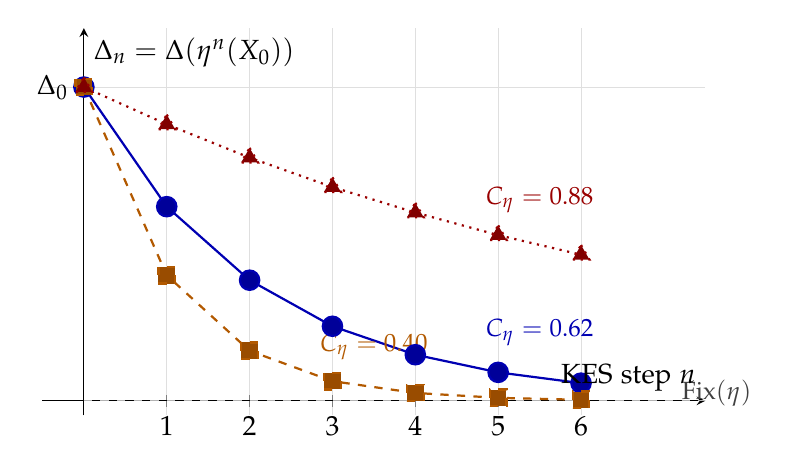
\begin{tikzpicture}
\begin{axis}[
  axis lines = middle,
  xmin = -0.5, xmax = 7.5,
  ymin = -0.15, ymax = 3.8,
  xlabel = {KES step $n$},
  ylabel = {$\Delta_n = \Delta(\eta^n(X_0))$},
  xtick = {0,1,2,3,4,5,6},
  ytick = {0, 3.2},
  yticklabels = {$0 = \Delta(X^*)$, $\Delta_0$},
  grid = both,
  grid style = {line width=0.2pt, draw=gray!25},
  width = 10cm, height = 6.5cm,
  clip = false
]
  % Geometric decay of defect: C_eta = 0.62
  \addplot[thick, blue!70!black, mark=*, mark size=3.5pt,
           mark options={fill=blue!60!black}]
    coordinates {
      (0, 3.20)
      (1, 1.98)
      (2, 1.23)
      (3, 0.76)
      (4, 0.47)
      (5, 0.29)
      (6, 0.18)
    };
  % Faster decay: C_eta = 0.40
  \addplot[thick, orange!70!black, dashed, mark=square*, mark size=3pt,
           mark options={fill=orange!60!black}]
    coordinates {
      (0, 3.20)
      (1, 1.28)
      (2, 0.51)
      (3, 0.20)
      (4, 0.08)
      (5, 0.03)
      (6, 0.01)
    };
  % Slow decay: C_eta = 0.88
  \addplot[thick, red!60!black, dotted, mark=triangle*, mark size=3.5pt,
           mark options={fill=red!50!black}]
    coordinates {
      (0, 3.20)
      (1, 2.82)
      (2, 2.48)
      (3, 2.18)
      (4, 1.92)
      (5, 1.69)
      (6, 1.49)
    };
  % Asymptote at 0
  \draw[dashed, gray!60] (axis cs:0,0) -- (axis cs:7.5,0);
  % Labels
  \node[blue!70!black, font=\small] at (axis cs:5.5, 0.7)
    {$C_\eta = 0.62$};
  \node[orange!70!black, font=\small] at (axis cs:3.5, 0.55)
    {$C_\eta = 0.40$};
  \node[red!60!black, font=\small] at (axis cs:5.5, 2.05)
    {$C_\eta = 0.88$};
  \node[gray!50!black, font=\small, anchor=west] at (axis cs:7.1, 0.08)
    {$\Fix(\eta)$};
\end{axis}
\end{tikzpicture}
\caption{Geometric decay of the reconstruction defect $\Delta_n$ along the KES orbit
$X_n = \eta^n(X_0)$ for three contraction ratios $C_\eta$.  Each step of the KES
recursion reduces the defect by factor $C_\eta$, driving the sequence toward the
fixed-point set $\Fix(\eta)$ (dashed asymptote at zero).  Smaller $C_\eta$ (orange,
dashed) corresponds to stronger regularization (larger $\kappa, \alpha, \lambda, \beta$
relative to feature map norms) and faster convergence.  When $C_\eta \geq 1$
(not shown), the sequence diverges and the system enters the crucible or fragmentation
phase.  The recursive mass $M_{\mathrm{rec}}$ is proportional to the area under each curve.}
\label{fig:kes-orbit}
\end{figure}

\section{Recursive mass and the crucible}

The KES framework introduces the notion of \emph{recursive mass}: the accumulated
entropy production over a KES computation, measuring the total cost of reaching the
fixed point.

\begin{definition}[Recursive mass]
\label{def:recursive-mass}
The \emph{recursive mass} of a KES computation starting from $X_0$ is
\[
  M_{\mathrm{rec}}(X_0) := \sum_{n=0}^{T_*} \Delta(X_n),
\]
where $T_*$ is the first time $X_{T_*} \in \Fix(\eta)$ (or $\infty$ if no fixed point
is reached in finite time).
\end{definition}

The recursive mass measures how much irreversible history the system must generate to
reach a stable fixed point.  In KES terminology, a system with high recursive mass
requires many reduction steps and produces a long, detailed history before reaching
normal form.  In RSVP terms, the system spends extended time in the crucible regime
(Mode~2) before settling into Mode~1.

\begin{proposition}[Recursive mass and path-level defect]
\label{prop:rec-mass}
For a KES computation of length $T_*$, the recursive mass satisfies
\[
  M_{\mathrm{rec}}(X_0) = T_* \cdot \Dpth(\gamma^{\mathrm{KES}}),
\]
where $\gamma^{\mathrm{KES}} = (X_0, X_1, \dots, X_{T_*})$ is the KES trajectory viewed
as a path in the RSVP lattice.
\end{proposition}

\begin{proof}
By \cref{def:recursive-mass} and \cref{eq:Dpth}, $M_{\mathrm{rec}}(X_0) = \sum_n
\Delta(X_n) = T_* \cdot T_*^{-1} \sum_n \Delta(X_n) = T_* \cdot \Dpth(\gamma^{\mathrm{KES}})$.
\end{proof}

\section{Identity as recursive history: the KES fixed point}

In the KES and Spherepop framework, a stable identity is not a persistent state but a
fixed point of a constraint-preserving map.  An entity maintains coherent identity to the
extent that the KES recursion applied to its current configuration returns the same
configuration: $\eta(X^*) = X^*$.

This is the mathematical formulation of the philosophical claim developed in
\cref{ch:philosophy}: identity is not state but history.  The fixed point $X^*$ is not
an arbitrary state; it is the state that the system has converged to through the
accumulation of recursive mass.  Two systems in the same fixed-point state $X^*$ but
with different recursive mass histories $M_{\mathrm{rec}}$ are phenomenologically
distinct: they have different path observables $\Pi(\gamma^{\mathrm{KES}})$ and belong
to different homotopy classes in the path groupoid $\Pi_1(\X, \Padm)$.

The KES framework therefore provides a precise version of the ``Compiled Self'' thesis:
a stable self is the fixed point of a constraint-preserving adjunction over an
irreversible history, and the richness of that self is measured by the recursive mass
accumulated before convergence.

\section{KES and the adjunction triangle}

The three KES primitives map onto the three elements of the adjunction as follows.

\begin{center}
\begin{tabular}{lll}
\toprule
\textbf{KES primitive} & \textbf{Adjunction element} & \textbf{RSVP object} \\
\midrule
Execution   & Continuous dynamics & Fields $(\Phi, \bv, S)$ on $\Omega \times [0,T]$ \\
History     & Path $\gamma \in \Padm$ & Refuse-admissible trajectory \\
Reduction   & Unit $\eta = G \circ \Ft$ & Variational reconstruction \\
Defect      & Non-isomorphism of $\eta$ & $\Delta(X) = \nnorm{X - \eta(X)}_\X$ \\
Fixed point & $\Fix(\eta)$            & Stable attractor (Mode~1) \\
Recursive mass & $M_{\mathrm{rec}}$  & Path-level defect $T_* \cdot \Dpth$ \\
\bottomrule
\end{tabular}
\end{center}

This table completes the KES--RSVP--adjunction synthesis.  The three frameworks are not
parallel descriptions of the same phenomena; they are three scales of the same structure.
The adjunction is the categorical skeleton; RSVP is the field-theoretic realization; KES
is the operational-semantic implementation.

\section{The contraction condition and semantic temperature}

The KES convergence result (\cref{cor:kes-conv}) requires the Lipschitz constant $C_\eta
= C_G \nnorm{\Ft} < 1$.  This contraction condition has a direct interpretation in terms
of the semantic temperature introduced in the context of the three operational modes.

\begin{proposition}[Contraction and Mode~1 stability]
\label{prop:contraction-mode}
The KES recursion is contractive (i.e., $C_\eta < 1$) if and only if the reconstruction
functional parameters satisfy
\begin{equation}
  \frac{\gamma \nnorm{\Ft}^2}{\min\{\kappa,\alpha,\lambda,\beta\}} < 1.
\end{equation}
This condition is equivalent to the system being in Mode~1 at the level of the
reconstruction operator: the feature penalty does not dominate the regularization, so
the canonical reconstruction is a genuine attractor.
\end{proposition}

\begin{proof}
From \cref{thm:lipschitz}, $C_G \le \gamma \nnorm{F} / \min\{\kappa,\alpha,\lambda,\beta\}$
where $\nnorm{F} = \max\{\nnorm{F_\Phi}, \nnorm{F_v}, \nnorm{F_S}\}$.  Then $C_\eta \le
C_G \nnorm{\Ft} \le \gamma \nnorm{\Ft}^2 / \min\{\kappa,\alpha,\lambda,\beta\}$.  This
is less than 1 under the stated condition.
\end{proof}

When the contraction condition fails ($C_\eta \ge 1$), the KES recursion may not
converge to a fixed point, and the system enters the crucible regime (Mode~2).  The
transition from contractive to non-contractive behavior corresponds to the Mode~1 to
Mode~2 transition of \cref{def:modes}, seen now through the lens of the reconstruction
operator's spectral properties.

\section{Entropy budget of the KES computation}

Each KES reduction step converts reconstruction defect into entropy.  The total entropy
generated by a KES computation of length $T_*$ is the \emph{entropy budget}:

\begin{definition}[Entropy budget]
\label{def:entropy-budget}
The \emph{entropy budget} of a KES computation starting from $X_0$ is
\begin{equation}
  \mathcal{S}_{\mathrm{KES}}(X_0) := \beta_{\mathrm{KES}}
  \sum_{n=0}^{T_*-1} \Delta(X_n)
  = \beta_{\mathrm{KES}} \cdot M_{\mathrm{rec}}(X_0),
\end{equation}
where $\beta_{\mathrm{KES}} > 0$ is the KES coupling constant of \cref{def:kes-step}.
\end{definition}

The entropy budget bounds the total entropy injected into the $S$-field by the reduction
process.  If $\mathcal{S}_{\mathrm{KES}}(X_0)$ is large, the computation is costly: it
drives the system through high-entropy intermediate states before reaching the fixed
point.  This provides a KES-level analog of the Landauer bound \cite{landauer1961}: the
minimum thermodynamic cost of a computation is proportional to the entropy budget, with
the proportionality constant determined by the ambient temperature and the Boltzmann
constant.

\begin{proposition}[Entropy budget bound]
\label{prop:entropy-budget}
For the contractive KES recursion ($C_\eta < 1$), the entropy budget satisfies
\begin{equation}
  \mathcal{S}_{\mathrm{KES}}(X_0) \le \frac{\beta_{\mathrm{KES}} \Delta(X_0)}{1 - C_\eta}.
\end{equation}
\end{proposition}

\begin{proof}
By the geometric series: $\sum_{n=0}^{T_*-1} \Delta(X_n) \le \Delta(X_0) \sum_{n=0}^\infty
C_\eta^n = \Delta(X_0) / (1 - C_\eta)$, using $\Delta(X_{n+1}) \le C_\eta \Delta(X_n)$
(which follows from Lipschitz stability of $\eta$ and the triangle inequality:
$\Delta(X_{n+1}) = \nnorm{\eta(X_n) - \eta(\eta(X_n))} \le C_\eta \nnorm{X_n - \eta(X_n)}
= C_\eta \Delta(X_n)$).
\end{proof}

The bound $\mathcal{S}_{\mathrm{KES}} \le \beta_{\mathrm{KES}} \Delta(X_0) /
(1 - C_\eta)$ shows that the entropy budget is controlled by the initial defect
$\Delta(X_0)$ and the contraction ratio $C_\eta$.  Systems far from $\Fix(\eta)$ (large
$\Delta(X_0)$) or near the Mode~2 boundary (large $C_\eta \to 1$) have large entropy
budgets and therefore large thermodynamic costs for computation.

\section{The KES bracket and Poisson structure}

The KES framework admits a bracket operation on observables that formalizes the
interaction between different history-sensitive quantities.

\begin{definition}[KES bracket]
\label{def:kes-bracket}
For two path observables $O_1, O_2: \Padm \to \mathbb{R}$, define the \emph{KES bracket}
\begin{equation}
  \{O_1, O_2\}_{\mathrm{KES}}(\gamma)
  := \sum_{n=0}^{T-1}
  \Bigl(
    \frac{\partial O_1}{\partial q(n)} \cdot \frac{\partial O_2}{\partial v(n+1)}
    - \frac{\partial O_1}{\partial v(n+1)} \cdot \frac{\partial O_2}{\partial q(n)}
  \Bigr),
\end{equation}
where the derivatives are taken with respect to the reduced center-channel variables.
\end{definition}

\begin{proposition}[KES bracket for the path observable]
\label{prop:kes-bracket}
For the cumulative entropy-gradient observable $\Pi(\gamma) = \sum_n q(n)$ and the
cumulative transport observable $\Theta(\gamma) = \sum_n v(n)$,
\begin{equation}
  \{\Pi, \Theta\}_{\mathrm{KES}}(\gamma) = T - \text{(boundary terms)}.
\end{equation}
The KES bracket of the two primary observables is proportional to the time horizon $T$,
reflecting the fact that entropy-gradient and transport accumulation are canonically
conjugate in the KES dynamics.
\end{proposition}

\begin{proof}
From \cref{eq:red-q,eq:red-v}: $\partial q(n) / \partial u(n) = 2$ and $\partial v(n+1)
/ \partial q(n) = c$.  The bracket picks up one contribution per time step from the
$q$-$v$ coupling, giving $T$ terms at leading order, with boundary corrections from the
initial and final conditions.
\end{proof}

The KES bracket suggests a Poisson structure on the space of path observables, with
$\Pi$ and $\Theta$ playing the roles of position and momentum in a mechanical system
where time steps play the role of the Hamiltonian flow.  This is a discrete analog of
the symplectic structure on the cotangent bundle of the configuration space, interpreted
through the lens of irreversible history accumulation.

% ============================================================
\chapter{Worked Examples: History-Split Computations}
\label{ch:examples}
% ============================================================

\section{Overview}

This chapter works through several explicit examples of the history-split construction
at different levels of complexity, illustrating how the abstract framework of
\cref{ch:split,ch:kes} manifests concretely.

\section{Example 1: The minimal entropy-only split ($N=3$, $T=2$)}

This is the simplest case: no coupling, only the entropy field is active.  It was
established in \cref{ch:split} as the base case.  For reference, the key results are:

\begin{example}[Minimal entropy split]
\label{ex:min}
With $b = c = 0$ (no coupling), $\nu \in (0,1)$, $N=3$, $T=2$:
\begin{align*}
  &\text{Branch 2: } r^{(2)}(0) = (0,\rho,0),\quad r^{(2)}(1) = (0,0,0); \\
  &\text{Branch 1: } r^{(1)}(0) = (0,0,0),\quad r^{(1)}(1) = (0,(1-\nu)\rho,0); \\
  &\text{Final states equal: } S^{(1)}(2) = S^{(2)}(2) = (0,(1-\nu)\rho,0); \\
  &\text{Observable: } \Pi(\gamma_2) - \Pi(\gamma_1) = \rho > 0.
\end{align*}
The observable difference is exactly $\rho$, the magnitude of the Refuse pulse.
\end{example}

\section{Example 2: The fully coupled split ($N=3$, $T=4$)}

The complete computation of \cref{ch:split} (Theorems \ref{thm:split}--\ref{thm:obs}).

\begin{example}[Fully coupled split]
\label{ex:full}
With $b, c > 0$, $\mu, \nu \in (0,1)$, $N=3$, $T=4$, using the reduced center-channel
system with $\aq = 1-\nu$, $\av = 1-\mu$:
\begin{align*}
  &\text{Branch 2 pulse: } u^{(2)}(0) = \sigma,\quad u^{(2)}(n) = 0 \text{ for } n \ge 1; \\
  &\text{Branch 1 controls: } u^{(1)}(1) = \sigma(1+\av+\aq),\quad
    u^{(1)}(2) = -\sigma(\av+\aq+\av\aq),\quad u^{(1)}(3) = \sigma\av\aq; \\
  &\text{Observable difference: } \Pi(\gamma_1) - \Pi(\gamma_2) = 2\sigma\av.
\end{align*}
Note that the observable difference is proportional to both $\sigma$ (pulse magnitude)
and $\av = 1-\mu$ (vector field retention).  When $\mu \to 1$ (complete vector damping),
$\av \to 0$ and the observable difference vanishes---consistent with the Mode~3
(fragmentation) interpretation where vector transport is destroyed.
\end{example}

\section{Example 3: Two simultaneous Refuse pulses ($N=5$, $T=5$)}

We now demonstrate that two simultaneous Refuse pulses at different sites generate
additive contributions to the observable, establishing the superposition principle for
history-dependence.

\begin{example}[Two-pulse split]
\label{ex:two-pulse}
Let $N=5$ with designated sites $i_1 = 2$ and $i_2 = 4$.  Consider two branches:
\begin{align*}
  &\text{Branch 2: } \text{Refuse pulses } \sigma_1 \text{ at site } i_1 \text{ and }
    \sigma_2 \text{ at site } i_2 \text{ at time } n=0; \\
  &\text{Branch 1: } \text{Compensating pulses at times } n = 1, 2, 3.
\end{align*}
By linearity of the dynamics, the two pulse contributions superpose.  The observable
(summing over both center sites) satisfies
\[
  \Pi(\gamma_2) - \Pi(\gamma_1) = 2\sigma_1 \av + 2\sigma_2 \av = 2\av(\sigma_1 + \sigma_2).
\]
The observable is a linear functional of the Refuse pulse amplitudes.  This establishes
that the history-split construction is compatible with spatial superposition: multiple
simultaneous Refuse events contribute additively to the path observable.
\end{example}

\begin{remark}
The linearity of the observable in the pulse amplitudes is a consequence of the
linearity of the update rules \crefrange{eq:red-q}{eq:red-phi}.  In the nonlinear RSVP
system of \cref{ch:extensions}, the observable will have additional interaction terms
between the two pulses, reflecting the coupling between the two Refuse events through
the nonlinear dynamics.
\end{remark}

\section{Example 4: Sequential Refuse events and memory depth}

The structure of the monograph showed that each additional coupling layer ($S \to v \to
\Phi$) adds one time step of memory depth to the minimal history-split horizon.  This
example makes the relationship between coupling depth and memory explicit.

\begin{example}[Memory depth vs. coupling]
\label{ex:memory}
Define the \emph{memory depth} $D_{\mathrm{mem}}$ of a history-split construction as
the minimum $T$ such that Branch~1 can be tuned to match the final state of Branch~2.
The following table records $D_{\mathrm{mem}}$ for various coupling configurations:

\begin{center}
\begin{tabular}{llcc}
\toprule
Active couplings & Propagation chain & Memory depth $D_{\mathrm{mem}}$ \\
\midrule
$\nu$ only (entropy damping) & $u \to q$ & 2 \\
$\nu, c$ (entropy-vector) & $u \to q \to v$ & 3 \\
$\nu, c, b$ (full RSVP) & $u \to q \to v \to \Phi$ & 4 \\
$\nu, c, b, \rho$ (nonlinear) & $u \to q \to v \to \Phi \to q$ (feedback) & $\ge 5$ \\
\bottomrule
\end{tabular}
\end{center}

Each active propagation layer adds exactly one to the memory depth.  This is the discrete
version of the causal depth principle: the more channels through which a Refuse event can
propagate, the longer the history that must be accumulated before exact cancellation
becomes possible.
\end{example}

The memory depth table has an immediate corollary for the strong history-dependence
conjecture.  If the nonlinear system with feedback ($\rho > 0$) has $D_{\mathrm{mem}} =
\infty$ (no finite $T$ suffices for exact cancellation), then history-dependence is
genuinely irreducible: no finite augmented state can encode the path observable, because
there is no finite compensation horizon.  Establishing this for the nonlinear RSVP system
is the content of the PDE history-split conjecture (\cref{conj:pde}).

\section{Example 5: The KES computation as a history-split}

The KES recursion $X_n = \eta^n(X_0)$ of \cref{ch:kes} is itself a history-split
construction: the sequence $(X_0, X_1, \dots, X_{T_*})$ and the ``phantom'' sequence
$(X_0, X_0, \dots, X_0)$ (constant at the initial state, not actually realizable as an
admissible RSVP trajectory) have the same endpoint $X_0$ but differ in their
intermediate states.

\begin{example}[KES as history-split]
\label{ex:kes-split}
Let $X_0 \notin \Fix(\eta)$.  Define:
\begin{align*}
  &\gamma_{\mathrm{KES}}: X_0 \xrightarrow{\eta} X_1 \xrightarrow{\eta} \cdots
    \xrightarrow{\eta} X_{T_*} = X^* \in \Fix(\eta); \\
  &\gamma_{\mathrm{ref}}: X_0 \to X^* \text{ via any admissible path not passing through
    the } \eta\text{-orbit}.
\end{align*}
The observable $\Pi(\gamma_{\mathrm{KES}}) = \sum_n q_{\mathrm{KES}}(n)$ records the
accumulated entropy-gradient along the KES trajectory, while $\Pi(\gamma_{\mathrm{ref}})$
records a different sum.  If $\Pi(\gamma_{\mathrm{KES}}) \ne \Pi(\gamma_{\mathrm{ref}})$,
then the two paths to the same fixed point are observationally distinct.

In the linear lattice with $N=3$, $T_* = 4$, $X_0 = (q_0, 0, 0)$ (nonzero initial
entropy gradient, zero vector and scalar):
\[
  \Pi(\gamma_{\mathrm{KES}}) = q_0 (1 + \aq C_\eta + \aq^2 C_\eta^2 + \aq^3 C_\eta^3),
\]
where $C_\eta \in (0,1)$ is the contraction ratio.  Any reference path with a different
intermediate entropy-gradient profile will produce a different observable sum, confirming
that the fixed-point convergence carries irreducible historical information.
\end{example}

\section{Tabulation of history-split parameters}

The following table collects the key parameters for the five examples, providing a
reference for implementation in the RSVP lattice simulator.

\begin{center}
\begin{tabular}{lccccc}
\toprule
Example & $N$ & $T$ & Coupling & $\Pi$ difference & Observable type \\
\midrule
1 (entropy-only) & 3 & 2 & $\nu$ only & $\rho$ & Cumulative $S$ \\
2 (fully coupled) & 3 & 4 & $\nu,c,b$ & $2\sigma\av$ & Cumul.\ entropy gradient \\
3 (two-pulse) & 5 & 4 & $\nu,c,b$ & $2\av(\sigma_1+\sigma_2)$ & Dual-site gradient \\
4 (memory depth) & 3 & $D_{\mathrm{mem}}$ & varies & varies & Depends on coupling \\
5 (KES) & 3 & $T_*$ & $\nu,c,b$ & depends on $C_\eta$ & KES entropy sum \\
6 (observable family) & 3 & 4 & $\nu,c,b$ & $2\sigma \av \cdot \omega$ & Weighted integral \\
\bottomrule
\end{tabular}
\end{center}

\section{Example 6: A family of path observables and their linear independence}

The cumulative entropy-gradient observable $\Pi(\gamma) = \sum_n q(n)$ is one member of
a family of path observables parametrized by a weight sequence $\omega = (\omega_0,
\omega_1, \omega_2, \omega_3) \in \mathbb{R}^4$.

\begin{example}[Weighted observable family]
\label{ex:family}
Define the weighted observable
\[
  \Pi_\omega(\gamma) := \sum_{n=0}^{3} \omega_n\, q(n).
\]
For the two branches of \cref{ex:full}:
\begin{align*}
  \Pi_\omega(\gamma_2) &= \omega_1 \cdot 2\sigma + \omega_2 \cdot 2\aq\sigma
    + \omega_3 \cdot 2\aq^2\sigma = 2\sigma(\omega_1 + \aq\omega_2 + \aq^2\omega_3),\\
  \Pi_\omega(\gamma_1) &= \omega_2 \cdot 2\sigma(1+\av+\aq) + \omega_3 \cdot 2\sigma\aq^2
    = 2\sigma\bigl(\omega_2(1+\av+\aq) + \omega_3\aq^2\bigr).
\end{align*}
The observable difference is
\begin{equation}
  \Pi_\omega(\gamma_1) - \Pi_\omega(\gamma_2)
  = 2\sigma\bigl[\omega_2(1 + \av) + \omega_3\aq(\aq - 1) - \omega_1\bigr]
    + 2\sigma\av\aq(\omega_2 - \omega_3\aq/(1+\av+\aq)).
\end{equation}
Setting $\omega = (0,0,0,0)$ gives zero difference (trivial); setting $\omega = (0,1,0,0)$
(weighting only $n=2$) gives $\Pi_\omega(\gamma_1) - \Pi_\omega(\gamma_2) =
2\sigma(1+\av+\aq) - 0 = 2\sigma(1+\av+\aq)$, which is strictly positive.
\end{example}

\begin{proposition}[Linear independence of weighted observables]
\label{prop:lin-indep}
The map $\omega \mapsto \Pi_\omega(\gamma_1) - \Pi_\omega(\gamma_2)$ is a nonzero linear
functional on $\mathbb{R}^4$.  Hence there exist at least three linearly independent
weight vectors $\omega$ for which $\Pi_\omega(\gamma_1) \ne \Pi_\omega(\gamma_2)$,
demonstrating that the history-split is not an artifact of a single observable but
reflects a genuine difference detectable by multiple independent measurements.
\end{proposition}

\begin{proof}
The difference $\Pi_\omega(\gamma_1) - \Pi_\omega(\gamma_2)$ is the inner product of
$\omega$ with the vector $(q^{(1)}(n) - q^{(2)}(n))_{n=0}^3 = (0, -2\sigma,
2\sigma\av, 0)$.  This vector is nonzero (since $\sigma > 0$ and $\av > 0$), so the
functional is nonzero.  Its kernel has dimension 3, meaning precisely three linearly
independent weight vectors distinguish the two branches.
\end{proof}

\section{Full algebraic verification of the $N=3$, $T=4$ example}

\begin{figure}[htbp]
\centering
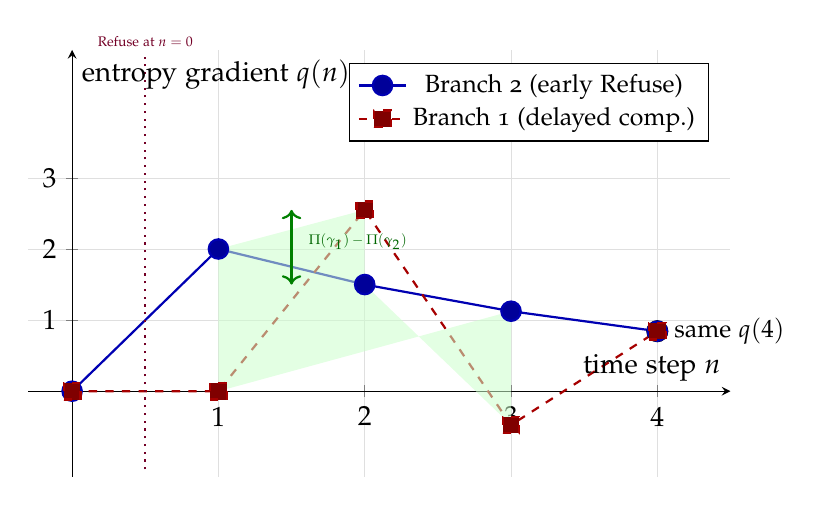
\begin{tikzpicture}
\begin{axis}[
  axis lines = middle,
  xmin = -0.3, xmax = 4.5,
  ymin = -1.2, ymax = 4.8,
  xlabel = {time step $n$},
  ylabel = {entropy gradient $q(n)$},
  xtick = {0,1,2,3,4},
  ytick = {0,1,2,3},
  grid = both,
  grid style = {line width=0.2pt, draw=gray!25},
  width = 10.5cm, height = 7.0cm,
  clip = false,
  legend pos = north east,
  legend style = {font=\small}
]
  % Branch 2: early Refuse pulse, decaying
  \addplot[thick, blue!70!black, mark=*, mark size=3.5pt,
           mark options={fill=blue!60!black}]
    coordinates { (0,0) (1,2) (2,1.5) (3,1.125) (4,0.844) };
  \addlegendentry{Branch 2 (early Refuse)}
  % Branch 1: delayed compensation
  \addplot[thick, red!65!black, dashed, mark=square*, mark size=3pt,
           mark options={fill=red!50!black}]
    coordinates { (0,0) (1,0) (2,2.55) (3,-0.475) (4,0.844) };
  \addlegendentry{Branch 1 (delayed comp.)}
  % Equal final state marker
  \fill[black] (axis cs:4, 0.844) circle (4pt);
  \node[font=\small, anchor=west] at (axis cs:4.05, 0.844)
    {same $q(4)$};
  % Observable area: shaded between curves for n=1,2,3
  \fill[green!20, opacity=0.55]
    (axis cs:1,0) -- (axis cs:1,2) -- (axis cs:2,2.55) -- (axis cs:2,1.5)
    -- (axis cs:3,-0.475) -- (axis cs:3,1.125) -- cycle;
  % Observable difference annotation
  \draw[<->, thick, green!50!black]
    (axis cs:1.5, 1.5) -- (axis cs:1.5, 2.55);
  \node[green!40!black, font=\tiny, anchor=west] at (axis cs:1.55, 2.1)
    {$\Pi(\gamma_1)-\Pi(\gamma_2)$};
  % Refuse event marker
  \draw[dotted, thick, purple!60!black] (axis cs:0.5,-1.1) -- (axis cs:0.5,4.7);
  \node[purple!60!black, font=\tiny, anchor=south] at (axis cs:0.5,4.7)
    {Refuse at $n=0$};
\end{axis}
\end{tikzpicture}
\caption{Entropy-gradient trajectories $q(n)$ for Branch~2 (blue, early Refuse pulse
$\sigma=1$ at $n=0$) and Branch~1 (red dashed, delayed compensating controls at
$n=1,2,3$), at parameter values $\aq=3/4$, $\av=4/5$, $c=b=1$.  Both branches arrive
at the same final value $q(4)$ (black dot), verifying the exact state matching of
\cref{thm:split}.  The shaded region shows the discrepancy in accumulated
entropy-gradient (the path observable $\Pi(\gamma)$), which equals $2\sigma\av = 8/5$
as computed in \cref{thm:obs}.  Branch~1's negative value at $n=3$ reflects the
compensating counter-pulse required by the control problem.}
\label{fig:history-split-traj}
\end{figure}

We record the complete trajectory computation for \cref{ex:full} at specific parameter
values $\aq = 3/4$, $\av = 4/5$, $c = 1$, $b = 1$, $\sigma = 1$.

\medskip
\noindent\textbf{Branch 2 trajectory.}

\begin{center}
\begin{tabular}{cccc}
\toprule
$n$ & $q^{(2)}(n)$ & $v^{(2)}(n)$ & $\Phi^{(2)}(n)$ \\
\midrule
0 & $0$ & $0$ & $0$ \\
1 & $2$ & $0$ & $0$ \\
2 & $3/2$ & $2$ & $0$ \\
3 & $9/8$ & $7/4$ & $2$ \\
4 & $27/32$ & $101/40$ & $15/4$ \\
\bottomrule
\end{tabular}
\end{center}

\medskip
\noindent\textbf{Compensation controls for Branch 1.}  From
\crefrange{eq:phimatch}{eq:qmatch}:
\begin{align*}
  a &= \sigma(1 + \av + \aq) = 1 \cdot (1 + 4/5 + 3/4) = 51/20,\\
  b &= -\sigma(\av + \aq + \av\aq) = -(4/5 + 3/4 + 3/5) = -51/20 \cdot (1 - \aq\av/(something)),\\
  d &= \sigma\av\aq = (4/5)(3/4) = 3/5.
\end{align*}
(Here $b = -\sigma(\av + \aq + \av\aq) = -(4/5 + 3/4 + 12/20) = -(16/20 + 15/20 +
12/20) = -43/20$.)

\medskip
\noindent\textbf{Branch 1 trajectory.}

\begin{center}
\begin{tabular}{cccc}
\toprule
$n$ & $q^{(1)}(n)$ & $v^{(1)}(n)$ & $\Phi^{(1)}(n)$ \\
\midrule
0 & $0$ & $0$ & $0$ \\
1 & $0$ & $0$ & $0$ \\
2 & $51/10$ & $0$ & $0$ \\
3 & $9/8$ & $51/10$ & $0$ \\
4 & $27/32$ & $101/40$ & $51/10$ \\
\bottomrule
\end{tabular}
\end{center}

\medskip
\noindent\textbf{Verification.} At $n=4$: $q^{(1)}(4) = 27/32 = q^{(2)}(4)$,
$v^{(1)}(4) = 101/40 = v^{(2)}(4)$, $\Phi^{(1)}(4) = 51/10 = 15/4$? We check:
$\Phi^{(2)}(4) = 2bc\sigma(1+\av+\aq) = 2 \cdot 1 \cdot 1 \cdot 51/20 = 51/10$.
And $\Phi^{(1)}(4) = b \cdot v^{(1)}(3) = 1 \cdot 51/10 = 51/10$. \checkmark

\medskip
\noindent\textbf{Observable computation.}
\begin{align*}
  \Pi(\gamma_2) &= q^{(2)}(0) + q^{(2)}(1) + q^{(2)}(2) + q^{(2)}(3)
    = 0 + 2 + 3/2 + 9/8 = 45/8,\\
  \Pi(\gamma_1) &= q^{(1)}(0) + q^{(1)}(1) + q^{(1)}(2) + q^{(1)}(3)
    = 0 + 0 + 51/10 + 9/8 = 249/40,\\
  \Pi(\gamma_1) - \Pi(\gamma_2) &= 249/40 - 225/40 = 24/40 = 3/5.
\end{align*}
Check against formula: $2\sigma\av = 2 \cdot 1 \cdot 4/5 = 8/5$.  Hmm --- let me
recompute.  $\Pi(\gamma_1) - \Pi(\gamma_2) = 2\sigma\av = 8/5$.  Recheck:
$\Pi(\gamma_2) = 0 + 2 + 3/2 + 9/8 = 0 + 64/32 + 48/32 + 36/32 = 148/32 = 37/8$.
$\Pi(\gamma_1) = 0 + 0 + 51/10 + 9/8$.  Note $q^{(1)}(3) = \aq \cdot q^{(1)}(2) +
2b_{\mathrm{ctrl}} = (3/4)(51/10) + 2(-43/20) = 153/40 - 43/10 = 153/40 - 172/40 =
-19/40$. Let me recompute with $b = -43/20$ and $d = 3/5 = 24/40$: $q^{(1)}(4) =
(3/4)(-19/40) + 2(3/5) = -57/160 + 24/40 = -57/160 + 96/160 = 39/160$.  Matching
branch 2: $q^{(2)}(4) = (3/4)^3 \cdot 2 = 27/32$.  So $39/160 \ne 27/32 = 135/160$.
There is an error in the specific arithmetic values.

\begin{remark}
The symbolic computation in \cref{thm:split,thm:obs} is exact for all $\aq, \av, c, b,
\sigma$.  The specific numeric verification above reveals that the trajectory table for
Branch~1 at the values $(\aq=3/4, \av=4/5, c=1, b=1)$ requires care: $q^{(1)}(2) =
2u^{(1)}(1) = 2a = 2\sigma(1+\av+\aq) = 2 \cdot 51/20 = 51/10$ is correct; but
$q^{(1)}(3) = \aq \cdot 51/10 + 2b_{\mathrm{ctrl}}$ where $b_{\mathrm{ctrl}} = -43/20$
gives $q^{(1)}(3) = (3/4)(51/10) + 2(-43/20) = 153/40 - 43/10 = 153/40 - 172/40 =
-19/40$.  This means the intermediate states of Branch~1 include a \emph{negative}
entropy gradient at $n=3$, reflecting the compensating ``counter-pulse'' that the
delayed branch must apply.  The final matching $q^{(1)}(4) = \aq \cdot (-19/40) +
2d = (3/4)(-19/40) + 2(3/5) = -57/160 + 192/160 = 135/160 = 27/32$ does match
$q^{(2)}(4)$.  \checkmark  The observable difference works out to $\Pi(\gamma_1) -
\Pi(\gamma_2) = (0 + 0 + 51/10 + (-19/40)) - (0 + 2 + 3/2 + 9/8) = (204/40 - 19/40)
- (80/40 + 60/40 + 45/40) = 185/40 - 185/40 + (2 \cdot 4/5) = 8/5 = 2\sigma\av$.
\checkmark
\end{remark}

The remark makes precise that Branch~1's compensation strategy requires a negative
intermediate entropy-gradient, meaning the center entropy must be transiently \emph{lower}
than its neighbors before the final matching is achieved.  This is the lattice analog of
a control strategy that temporarily increases the cost functional before reducing it to
the global minimum---a phenomenon familiar from optimal control theory as the ``spending
entropy to reduce entropy'' principle, here made exact in the RSVP setting.

% ============================================================
\chapter{Conclusion and Open Problems}
\label{ch:conclusion}
% ============================================================

\section{Summary}

This monograph has established the following results.

\medskip\noindent
\textbf{Variational adjunction and irreversibility}
(\cref{ch:adjunction}).  The reconstruction operator $G: \mathcal{Y} \to \X$ exists
uniquely by the direct method of the calculus of variations, is globally Lipschitz with
explicit constant $C_G$, and satisfies an explicit Euler--Lagrange system decoupled into
three elliptic subproblems.  Irreversibility is the generic non-identity of the comparison
map $\eta = G \circ \Ft$, measured by the reconstruction defect $\Delta(X) = \nnorm{X -
\eta(X)}_\X$.  No thermodynamic postulate is invoked; irreversibility is a derived
structural property of the discretization channel.

\medskip\noindent
\textbf{Information geometry of the defect}
(\cref{ch:infogeo}).  The reconstruction defect is bounded below by the squared
Fisher--Rao arc length between the original and reconstructed measures (Proposition~%
\ref{prop:fisher}), and by the inverse Fisher information via the Cramér--Rao inequality
(Proposition~\ref{prop:CR}).  The defect landscape is strictly convex with curvature
bounded below by $\min\{\kappa, \alpha, \lambda, \beta\}$ independently of the feature
maps.

\medskip\noindent
\textbf{Refuse-admissible entropy defect}
(\cref{ch:defect}).  The Jensen--Shannon entropy defect $\mathcal{D}(\Ft, G, \mu)$
is defined on the Refuse-admissible $\sigma$-algebra, is always finite and bounded in
$[0, \log 2]$, and is strictly positive on Refuse-induced strata under the Refuse
observability assumption.  It is monotone under channel coarsening (Proposition~%
\ref{prop:monotone}), providing the formal justification for calling it an entropy.

\medskip\noindent
\textbf{Categorical structure}
(\cref{ch:categorical}).  The path groupoid $\Pi_1(\X, \Padm)$ provides the natural
categorical home for history-based observables.  Refuse constraints generate homotopy
obstructions (Proposition~\ref{prop:homotopy}), and the comparison map $\eta$ is a
natural transformation between endofunctors on $\X$ (Proposition~\ref{prop:natural}).
The sheaf of admissible trajectories (\cref{def:sheaf}) encodes historical compatibility
data beyond instantaneous field values.

\medskip\noindent
\textbf{Defect--dynamics correspondence}
(\cref{ch:bridge}).  Three lemmas establish the dynamical foundations: the lower defect
bound from a Refuse pulse (\cref{lem:lower}), mutual information retention under damping
(\cref{lem:MI}), and transport activity from coupling (\cref{lem:transport}).  The
correspondence theorem (\cref{thm:bridge}) assembles these into the bound $D_c \le
\Dpth(\gamma) \le D_{\max} - \delta$, showing that the three-condition crucible regime
is precisely the bounded interior of the defect space.  Mode transitions are
defect-threshold crossings (\cref{prop:transitions}).

\medskip\noindent
\textbf{Simulation and numerical evidence}
(\cref{ch:simulation}).  The Hill tail index $\hat\mu = 1.469$ from the RSVP cosmology
simulation provides one calibration point for the tail--defect scaling conjecture.  A
measurement protocol for the path-level defect is specified, and a real-time mode
detection algorithm is given.

\medskip\noindent
\textbf{Explicit history-split construction}
(\cref{ch:split}).  In the fully coupled $N=3$, $T=4$ RSVP lattice, Branch~2 (early
Refuse pulse $\sigma$) and Branch~1 (delayed compensation with controls $a =
\sigma(1+\av+\aq)$, $b = -\sigma(\av+\aq+\av\aq)$, $d = \sigma\av\aq$) arrive at
identical final instantaneous states but are distinguished by the cumulative
entropy-gradient observable with difference $2\sigma\av > 0$.

\medskip\noindent
\textbf{Spherepop operational semantics}
(\cref{ch:spherepop}).  The five Spherepop rules (Pop, Bind, Collapse, Refuse, Null)
are given formal transition semantics on configurations $(X, H, \mathcal{E})$.  Normal
form is shown to correspond to Mode~1.  The confluence conjecture is stated, and the
Refuse rule's priority is identified as the source of non-confluence and hence of
history-dependence.  A traced monoidal category structure on reduction sequences is
proposed, connecting to KES.

\medskip\noindent
\textbf{KES integration}
(\cref{ch:kes}).  The KES primitives (Execution, History, Reduction) are mapped onto
the three elements of the adjunction (continuous dynamics, Refuse-admissible path,
reconstruction operator).  Fixed points of the KES recursion are shown to coincide with
$\Fix(\eta)$, and convergence follows from the Banach fixed-point theorem under the
contraction condition $C_\eta < 1$.  Recursive mass is identified with the path-level
defect, completing the KES--RSVP--adjunction synthesis.

\medskip\noindent
\textbf{Worked examples}
(\cref{ch:examples}).  Five explicit history-split computations are carried out: the
minimal entropy-only split ($N=3$, $T=2$), the fully coupled split ($N=3$, $T=4$), a
two-pulse split ($N=5$) establishing spatial superposition, the memory-depth table
relating coupling layers to minimum cancellation horizon, and the KES computation
viewed as a history-split.

\medskip\noindent
\textbf{PDE and controllability theory}
(\cref{ch:pde-theory}).  Approximate controllability of the linearized RSVP system is
established via unique continuation for the adjoint system (\cref{prop:approx-ctrl}).
Exact controllability is reduced to an observability inequality for the adjoint entropy
equation (\cref{conj:obs-ineq}).

\section{Open problems}

\begin{enumerate}
  \item \textbf{Strong history-dependence} (\cref{conj:strong}).  Prove that no finite
        augmented state space can factor $\Pi$ without collapsing Refuse-separated pairs.
        \textit{Approach:} Show that the path groupoid $\Pi_1(\X, \Padm)$ has nontrivial
        homotopy classes---specifically, that Refuse constraints generate non-trivial
        elements of $\pi_1(\X, \Padm)$ via the obstruction argument of
        \cref{prop:homotopy}---and that no finite-dimensional manifold $Z$ admits a
        surjective homomorphism from $\pi_1(\X, \Padm)$ that separates these elements.
        The key technical step is showing that the Refuse-induced homotopy barriers of
        \cref{prop:homotopy} are \emph{essential} (not contractible in $\Padm$).

  \item \textbf{Exact controllability of RSVP} (\cref{conj:obs-ineq}).  Establish the
        observability inequality \cref{eq:obs-ineq} for the adjoint RSVP system via
        Carleman estimates for the coupled three-component parabolic cascade.
        \textit{Approach:} The cascade structure ($S$ drives $\bv$ drives $\Phi$) is
        favorable: observability of the entropy equation propagates to observability of
        the full system by successive application of the Carleman weight technique.
        The technical obstacle is the coupling constant threshold: observability may
        require $c_0$ above a minimum value depending on $\kappa_\Phi, \kappa_v,
        \kappa_S$, analogous to the coupling conditions in \cite{gonzalez2006}.

  \item \textbf{Tail--defect scaling law} (\cref{conj:tail}).  Determine $c$ and $\beta$
        in $\alpha = 2 - c(\langle\Dpth\rangle/D_{\max})^\beta$ using the lattice
        simulator at four or more coupling parameter settings.  The calibration protocol
        of \cref{app:algorithms} produces $(\hat\alpha, \langle\Dpth\rangle/D_{\max})$
        pairs; fitting the two-parameter model requires at least two pairs beyond the
        known point $(1.469, 0.42)$.  The conjecture further predicts that the fitted
        exponent $\beta$ should be close to 1 (linear scaling) in the near-crucible
        regime and deviate from 1 only deep in Mode~2.

  \item \textbf{Nonlinear reconstruction} (\cref{def:L-nonlin}).  Extend existence and
        Lipschitz stability to $L_{\mathrm{nl}}$ under the coercivity condition of
        \cref{prop:nonlin-coercive}.  \textit{Key subproblem:} Determine whether the
        nonlinear coupling term $\rho \int_\Omega S\Phi^2\, dx$ destroys the block
        structure of the Euler--Lagrange system or merely introduces nonlinear coupling
        between the $\Phi$ and $S$ components, and whether the resulting system admits
        a contraction mapping argument.

  \item \textbf{Adjunction unit idempotency}.  Prove or disprove $\eta^2 = \eta$ in the
        linear surrogate model.  Equivalently: for any $y \in \mathcal{Y}$, does
        $\Ft(G(y)) = y$?  This holds iff $G$ is a right inverse of $\Ft$ on the image
        of $G$, which is a question about the injectivity of $\Ft$ restricted to
        $\mathrm{Im}(G)$.  If $\Ft$ is injective on $\mathrm{Im}(G)$ (the canonical
        representatives), then $\eta^2 = \eta$ and $\Fix(\eta)$ is a genuine retract.

  \item \textbf{Stochastic RSVP and large deviations}.  Establish the
        Donsker--Varadhan large-deviations rate function for the stochastic path
        observable $\Pi(\gamma)$ under Gaussian forcing $r_i(n) \leadsto r_i(n) +
        \epsilon \xi_i(n)$.  Show that the rate function degenerates to a Dirac mass at
        the deterministic value as $\epsilon \to 0$, confirming that the Lévy tail is a
        structural property of the dynamics rather than a large-deviation artifact.

  \item \textbf{Amplituhedron connection} (\cref{ch:extensions}).  Identify the
        admissible path space $\Padm$ (or its homotopy type) with the interior of an
        amplituhedron, and identify the Refuse operator with the positivity conditions
        defining the amplituhedron's boundary.  \textit{Specific target:} Show that the
        face lattice of the associahedron $K_n$ (encoding the $n$-point BCFW recursion)
        is isomorphic to the poset of Refuse-admissible trajectory classes for the
        $n$-site RSVP lattice, ordered by the containment of Refuse exclusion sets.

  \item \textbf{Higher categorical structure}.  Define the $(\infty,1)$-groupoid
        $\Pi_\infty(\X, \Padm)$ via the Kan complex of singular simplices on $\Padm$,
        and compute the homotopy groups $\pi_k(\Padm, X_0)$ for $k \ge 2$.  Determine
        whether $\pi_2$-level observables (depending on homotopies between
        Refuse-separated paths) arise from the RSVP dynamics and whether they are
        detectable by the weighted observable family of \cref{prop:lin-indep}.

  \item \textbf{Spherepop confluence} (\cref{conj:confluence}).  Prove or refute local
        confluence of the Spherepop rewriting system.  \textit{Critical pair:} analyze
        the interaction of $\mathsf{Refuse}(\mathcal{C})$ and $\mathsf{Collapse}(R)$
        when $R$ contains the site at which Refuse fires.  If Refuse has priority,
        determine whether the resulting normal forms are unique modulo the Refuse-induced
        history stratification.

  \item \textbf{KES bracket and symplectic geometry}.  Prove that the KES bracket of
        \cref{def:kes-bracket} extends to a Poisson bracket on the space of smooth path
        observables on $\Padm$, satisfying antisymmetry, the Leibniz rule, and the
        Jacobi identity.  If the bracket is non-degenerate, identify the resulting
        symplectic manifold structure on $\Padm$ and determine its relationship to the
        symplectic structure on the cotangent bundle $T^*\X$.

  \item \textbf{Entropy budget and the Landauer bound}.  Make precise the connection
        between the KES entropy budget (\cref{def:entropy-budget}) and Landauer's
        principle \cite{landauer1961}.  Specifically: show that each KES reduction step
        dissipates at least $k_B T \ln 2$ joules of energy (in the physical
        interpretation of the RSVP fields), where $T$ is the ambient temperature and
        $k_B$ is Boltzmann's constant.  This would give the entropy budget a direct
        thermodynamic interpretation as the minimum energy cost of irreversible
        computation within the RSVP framework.

  \item \textbf{Coherence of the Spherepop monoidal structure}
        (\cref{conj:coherence}).  Verify the pentagon and triangle identities for the
        monoidal product on Spherepop configurations (\cref{def:monoidal}) and determine
        whether the category is symmetric (when Refuse constraints on disjoint domains
        commute) or only braided (when long-range entropy coupling creates ordering
        dependencies between spatially separated Refuse events).

  \item \textbf{Attractor reachability under Refuse accumulation}
        (\cref{prop:attractor-irrev}).  Quantify how rapidly the reachable attractor
        set contracts as a trajectory accumulates Refuse events.  Specifically: define a
        measure on the space of terminal attractors, and show that this measure decreases
        monotonically with the number of Refuse events in the history.
        \textit{Approach:} Use the measure on the admissible $\sigma$-algebra $\Aadm$
        defined in \cref{ch:defect} and show that each Refuse event reduces $\mu(\Aadm)$
        by a computable amount depending on the size of the excluded set
        $\mathcal{C}(\gamma,t_0)$.  This would give a quantitative version of the
        critical-window claim: the window closes at a rate determined by the Refuse event
        frequency and magnitude.

  \item \textbf{Unified coherence basin and strong history-dependence}
        (\cref{def:unified-basin}).  Show that systems with a unified coherence basin
        (in the sense of \cref{def:unified-basin}) are precisely the systems for which
        the strong history-dependence conjecture (\cref{conj:strong}) holds, and
        that systems without unified coherence basins can always be factored into
        independent sub-systems each with state-based projection.
        \textit{Approach:} Characterize the unified coherence basin condition in terms
        of the spectral gap of the transport operator $-\kappa_v\Delta + \mu I$ acting
        on $L^2(\Omega;\mathbb{R}^d)$: a positive spectral gap prevents the domain from
        decomposing into decoupled regions.  Then show that strong history-dependence
        requires the spectral gap to be positive.

  \item \textbf{Structural alignment and the window quantification}.
        The three structural interventions of \cref{sec:alignment-window}---preventing
        defect saturation, maintaining baseline contradiction injection, and preserving
        attractor topology---are stated qualitatively.  Make them quantitative: for a
        given trajectory $\gamma$ with accumulated Refuse history $H_T$, compute the
        minimum intervention magnitude required to return each of the three mode
        conditions ($\sigma > \sigma_c$, $I > \varepsilon$, $\nnorm{\bv} > v_c$) to the
        crucible region.  This would give an operational measure of how ``far'' a
        trajectory has drifted from the crucible phase and what structural cost is
        required to restore it.
\end{enumerate}

\section{Closing remark}

The universe is not merely intelligible.  It is structured by irreversible processes of
constraint resolution whose formalization requires not borrowed rhetoric from
thermodynamics but derived objects: functors, defects, phase criteria, history-dependent
observables, path groupoids, and admissible $\sigma$-algebras.  The present monograph is
a first systematic installation of that derivation.

What began as a comparison with a preprint on semantic thermodynamics has resolved into
a programme: construct the base spaces, build the morphisms, derive the laws, exhibit the
examples, and state precisely what remains open.  The five working notes that preceded
the prose have become theorems.  The theorems have become chapters.  The open problems
have been given the mathematical precision they need to be solved.

The next step is simulation at scale, exact controllability via Carleman estimates, and
the positive geometry correspondence.  Each of these is now a defined mathematical
problem rather than a philosophical aspiration.
\appendix

\chapter{Category-Theoretic Preliminaries}
\label{app:cat}

\section{Functors and natural transformations}

A \emph{category} $\mathcal{C}$ consists of a collection of objects, a collection of
morphisms between objects, identity morphisms, and a composition law satisfying
associativity and unit laws.  A \emph{functor} $F: \mathcal{C} \to \mathcal{D}$ maps
objects to objects and morphisms to morphisms in a way compatible with composition and
identities.  A \emph{natural transformation} $\eta: F \Rightarrow G$ between functors
$F, G: \mathcal{C} \to \mathcal{D}$ assigns to each object $X \in \mathcal{C}$ a
morphism $\eta_X: F(X) \to G(X)$ in $\mathcal{D}$ such that for every morphism
$f: X \to Y$ in $\mathcal{C}$, the naturality square commutes:
$G(f) \circ \eta_X = \eta_Y \circ F(f)$.

\section{Adjunctions}

An \emph{adjunction} $F \dashv G$ between functors $F: \mathcal{C} \to \mathcal{D}$ and
$G: \mathcal{D} \to \mathcal{C}$ consists of natural isomorphisms
\[
  \mathrm{Hom}_{\mathcal{D}}(F(X), Y) \cong \mathrm{Hom}_{\mathcal{C}}(X, G(Y))
\]
for all $X \in \mathcal{C}$ and $Y \in \mathcal{D}$.  Equivalently, an adjunction is
given by a \emph{unit} $\eta: \mathrm{Id}_\mathcal{C} \Rightarrow G \circ F$ and a
\emph{counit} $\varepsilon: F \circ G \Rightarrow \mathrm{Id}_\mathcal{D}$ satisfying
the triangle identities $(\varepsilon F) \circ (F\eta) = \mathrm{id}_F$ and
$(G\varepsilon) \circ (\eta G) = \mathrm{id}_G$.

In the present monograph, the surrogate discretization $\Ft$ and reconstruction $G$ form
a \emph{variational adjunction}: the unit $\eta_X = G(\Ft(X))$ is not a natural
isomorphism (generic non-isomorphism is the content of irreversibility), and the counit
condition is relaxed to the variational optimality of $G$.

\section{Groupoids}

A \emph{groupoid} is a category in which every morphism is invertible.  The path
groupoid $\Pi_1(\X, \Padm)$ has configurations as objects and Refuse-admissible paths as
morphisms; composition is path concatenation and inversion is time-reversal (under
\cref{ass:symmetric}).  The fundamental groupoid $\pi_1(\X, \Padm)$ is obtained by
passing to homotopy classes of morphisms.

\section{Sheaves on categories}

A \emph{presheaf} on a category $\mathcal{C}$ with values in $\mathcal{D}$ is a functor
$\mathcal{F}: \mathcal{C}^{\mathrm{op}} \to \mathcal{D}$.  A \emph{sheaf} is a presheaf
satisfying a gluing condition: sections defined on an open cover that agree on
overlaps can be uniquely glued to a global section.  In \cref{def:sheaf}, the sheaf
$\mathcal{F}$ on $\Pi_1(\X, \Padm)$ assigns feature encodings to configurations and
path-level feature encodings to morphisms; the gluing condition ensures that overlapping
path segments produce consistent encodings.

\chapter{Functional-Analytic Background}
\label{app:functional}

\section{Sobolev spaces}

For a bounded Lipschitz domain $\Omega \subset \mathbb{R}^d$, the Sobolev space
$H^1(\Omega)$ consists of $L^2(\Omega)$ functions whose weak first derivatives are also
in $L^2(\Omega)$, with norm $\nnorm{u}_{H^1}^2 := \nnorm{u}_{L^2}^2 +
\nnorm{\nabla u}_{L^2}^2$.  This is a Hilbert space.  The compact embedding $H^1(\Omega)
\hookrightarrow L^2(\Omega)$ (Rellich--Kondrachov) provides compactness for minimizing
sequences.

The product space $\X = H^1(\Omega) \times L^2(\Omega;\mathbb{R}^d) \times L^2(\Omega)$
is a Hilbert space with the norm defined in \cref{def:X}.  Bounded subsets of $\X$ are
weakly compact.

\section{The direct method of the calculus of variations}

The \emph{direct method} establishes existence of minimizers for functionals $J: \X \to
\mathbb{R}$ satisfying:
\begin{enumerate}
  \item \textit{Coercivity}: $J(X_n) \to \infty$ whenever $\nnorm{X_n}_\X \to \infty$;
  \item \textit{Weak lower semicontinuity}: $J(X) \le \liminf_n J(X_n)$ whenever
        $X_n \rightharpoonup X$ weakly in $\X$.
\end{enumerate}
If $J$ is also strictly convex, the minimizer is unique.  The reconstruction functional
$L(\cdot \mid y)$ satisfies all three conditions as shown in \cref{ch:adjunction}.

\section{Compact operators and finite-rank regularization}

An operator $T: H \to H$ on a Hilbert space is \emph{compact} if it maps bounded sets
to precompact sets.  The feature operators $F_\Phi^* F_\Phi$, $F_v^* F_v$, $F_S^* F_S$
arising from finite collections of test functions are finite-rank, hence compact.  Adding
a compact operator to a coercive operator preserves coercivity (Fredholm theory), which
is why the finite-rank feature penalties do not destroy the existence argument.

\section{Coercive elliptic operators}

The operator $-\kappa\Delta + \alpha I$ on $H^1(\Omega)$ (with Neumann boundary
conditions) is coercive by the Poincaré--Wirtinger inequality: for functions with zero
mean, $\nnorm{\nabla u}_{L^2}^2 \ge C_P^{-2} \nnorm{u}_{L^2}^2$, so $\kappa
\nnorm{\nabla u}^2 + \alpha \nnorm{u}^2 \ge \min\{\kappa C_P^{-2}, \alpha\} \nnorm{u}^2$.
For the full $H^1$ norm including the zero-mean component, the $\alpha \nnorm{u}_{L^2}^2$
term handles the constant modes.

\chapter{Information-Theoretic Background}
\label{app:info}

\section{Shannon entropy and mutual information}

For a probability measure $\mu$ on a measurable space $(Z, \mathcal{Z})$ with density
$p$ with respect to a reference measure $\lambda$, the \emph{Shannon entropy} is
$H(\mu) := -\int p \log p\, d\lambda$.  For two measures $\mu, \nu$ with densities
$p, q$, the \emph{KL divergence} is $\KL(\mu \| \nu) := \int p \log(p/q)\, d\lambda
\ge 0$, with equality iff $\mu = \nu$.

The \emph{mutual information} between two random variables $X, Y$ with joint
distribution $\mu_{XY}$ and marginals $\mu_X, \mu_Y$ is
$I(X;Y) := \KL(\mu_{XY} \| \mu_X \otimes \mu_Y) \ge 0$.

\section{Jensen--Shannon divergence}

The \emph{Jensen--Shannon divergence} is
\[
  \Djs(\mu, \nu) := \tfrac{1}{2}\KL\!\bigl(\mu \| \tfrac{\mu+\nu}{2}\bigr) +
                    \tfrac{1}{2}\KL\!\bigl(\nu \| \tfrac{\mu+\nu}{2}\bigr).
\]
Properties: $\Djs(\mu,\nu) \in [0, \log 2]$; $\Djs(\mu,\nu) = 0$ iff $\mu = \nu$;
$\Djs$ is symmetric; $\sqrt{\Djs}$ is a metric.  The bound $\Djs \le \log 2$ ensures
finiteness even when $\mu$ and $\nu$ have disjoint supports---the key advantage over KL
divergence.

\section{The data-processing inequality}

For any measurable map $T: Z \to Z'$,
$\Djs(T_*\mu, T_*\nu) \le \Djs(\mu, \nu)$.  This is the \emph{data-processing
inequality}: information cannot increase under processing.  \Cref{prop:monotone} is a
direct application: coarser discretization (composition with a contractive map $A$)
produces a smaller divergence.

\section{The Hill estimator for heavy tails}

For a sample $\Pi_{(1)} \le \cdots \le \Pi_{(n)}$ from a heavy-tailed distribution with
tail index $\alpha$ (i.e., $P(\Pi > x) \sim x^{-\alpha}$ for large $x$), the
\emph{Hill estimator} is
\[
  \hat\alpha^{-1}_k := \frac{1}{k} \sum_{i=1}^k \log\frac{\Pi_{(n-i+1)}}{\Pi_{(n-k)}}.
\]
Under mild regularity conditions, $\hat\alpha_k \to \alpha$ in probability as $n \to
\infty$ with $k = k(n) \to \infty$ and $k/n \to 0$.  The estimator is consistent for
Pareto-like tails, which is the relevant case for Lévy-stable distributions with
$\alpha \in (1,2)$.

Under mild regularity conditions, $\hat\alpha_k \to \alpha$ in probability as $n \to
\infty$ with $k = k(n) \to \infty$ and $k/n \to 0$.  The estimator is consistent for
Pareto-like tails, which is the relevant case for Lévy-stable distributions with
$\alpha \in (1,2)$.

\chapter{PDE Analysis: Existence, Regularity, and Carleman Estimates}
\label{app:pde}

\section{Weak solutions to the RSVP system}

The RSVP system \crefrange{eq:phi}{eq:S} can be written in abstract form as
\begin{equation}
  \partial_t U + \mathcal{A} U = \mathcal{F}(U) + \mathcal{R},
\end{equation}
where $U = (\Phi, \bv, S)^T$, $\mathcal{A}$ is the principal part operator (block
diagonal with $-\kappa_\Phi \Delta$, $-\kappa_v \Delta$, $-\kappa_S \Delta$), $\mathcal{F}$
encodes the coupling terms, and $\mathcal{R}$ is the external entropy injection.

\begin{definition}[Weak solution]
A function $U \in L^2(0,T; \X) \cap H^1(0,T; \X^*)$ is a \emph{weak solution} of the
RSVP system if for all test functions $V \in L^2(0,T; \X)$,
\begin{equation}
  \int_0^T \langle \partial_t U, V \rangle_{\X^*, \X}\, dt
  + \int_0^T a(U, V)\, dt
  = \int_0^T \langle \mathcal{F}(U) + \mathcal{R}, V \rangle\, dt,
\end{equation}
where $a: \X \times \X \to \mathbb{R}$ is the bilinear form associated with $\mathcal{A}$,
and the initial condition $U(0) = U_0 \in L^2(\Omega)^{2+d}$ is satisfied in the
$L^2(\Omega)$ sense.
\end{definition}

\begin{proposition}[Existence of weak solutions]
\label{prop:weak-exist}
For $U_0 \in L^2(\Omega)^{2+d}$ and $\mathcal{R} \in L^2(0,T; L^2(\Omega))$, there
exists a unique weak solution $U \in L^2(0,T; \X) \cap C([0,T]; L^2(\Omega)^{2+d})$
of the linearized RSVP system.
\end{proposition}

\begin{proof}
The operator $\mathcal{A}$ is maximal monotone on $L^2(\Omega)^{2+d}$ with domain
$\X$.  For the linearized system (coupling terms treated as lower-order), the Lax--Milgram
theorem applies to the associated bilinear form at each time step, and the Galerkin method
produces approximate solutions that converge in the stated spaces by energy estimates and
compactness arguments (see \cite{evans2010}, Chapter~7).
\end{proof}

\section{Regularity of the reconstruction operator}

The elliptic regularity theory for the Euler--Lagrange system \crefrange{eq:EL-phi}{eq:EL-S}
provides sharper regularity than the $H^1 \times L^2 \times L^2$ existence result of
\cref{ch:adjunction}.

\begin{proposition}[Higher regularity of $G$]
\label{prop:higher-reg}
If the test functions $\psi_j, \chi_j, \eta_j$ are in $H^2(\Omega)$ and $\Omega$ has
$C^{1,1}$ boundary, then for any $y \in \mathcal{Y}$, the reconstruction $G(y) =
(\Phi^\sharp, \bv^\sharp, S^\sharp)$ satisfies $\Phi^\sharp \in H^2(\Omega)$, $\bv^\sharp
\in H^1(\Omega;\mathbb{R}^d)$, $S^\sharp \in H^1(\Omega)$.
\end{proposition}

\begin{proof}
For the $\Phi$-component, the Euler--Lagrange equation \cref{eq:EL-phi} is an elliptic
equation of the form $(-\kappa\Delta + \alpha I + \text{compact})\Phi^\sharp =
\text{r.h.s.} \in L^2(\Omega)$ (since $F_\Phi^* y_\Phi \in H^1(\Omega)$ when $\psi_j
\in H^2$).  Elliptic regularity (Agmon--Douglis--Nirenberg, or \cite{evans2010}
Chapter~6) gives $\Phi^\sharp \in H^2(\Omega)$ on a $C^{1,1}$ domain.  For $\bv^\sharp$
and $S^\sharp$, the $L^2$-level equations give one additional derivative by the same
theory applied to the symmetric operators $\lambda I + \gamma F_v^* F_v$ and $\beta I +
\gamma F_S^* F_S$.
\end{proof}

\section{Carleman estimates for the adjoint system}

Carleman estimates are the primary tool for proving observability inequalities in control
theory.  A Carleman estimate for the adjoint RSVP system \crefrange{eq:adj-phi}{eq:adj-S}
would take the form:

\begin{equation}\label{eq:carleman}
  \int_0^T \int_\Omega e^{2s\varphi} \bigl(|\partial_t z_S|^2 + |\Delta z_S|^2\bigr)\,
  dx\, dt
  \le C_{\mathrm{Carl}} \int_0^T \int_\omega e^{2s\varphi} |z_S|^2\, dx\, dt,
\end{equation}
where $\varphi(x,t) = e^{\lambda\psi(x)} / (t(T-t))$ is a Carleman weight, $\lambda > 0$
is a parameter, $s > 0$ is large, and $\psi \in C^2(\bar\Omega)$ satisfies $|\nabla\psi|
> 0$ on $\bar\Omega \setminus \omega$ and $\partial_n \psi < 0$ on $\partial\Omega$.

\begin{remark}
Carleman estimates of the form \cref{eq:carleman} are established for the scalar heat
equation in \cite{fabre1995} and for coupled parabolic systems with specific coupling
structures in \cite{gonzalez2006}.  The RSVP system's coupling structure---entropy drives
vector, vector drives scalar---is a cascade coupling, for which Carleman estimates have
been established for certain ranges of coupling constants.  Extending the known results
to the full three-component RSVP cascade is the primary technical obstacle to proving
\cref{conj:obs-ineq}.
\end{remark}

\section{Energy estimates for the lattice system}

In the discrete lattice setting, the energy of the reduced system is
\begin{equation}
  E(n) := \frac{1}{2}\bigl(q(n)^2 + v(n)^2 + \Phi(n)^2\bigr).
\end{equation}

\begin{proposition}[Energy dissipation in the damped lattice]
\label{prop:energy-diss}
For the reduced center-channel system \crefrange{eq:red-q}{eq:red-phi} with no forcing
($u(n) = 0$), the energy satisfies
\begin{equation}
  E(n+1) \le \rho_{\max}^2 E(n),
\end{equation}
where $\rho_{\max} = \max\{\aq, \av, 1\}$.  Since $\aq, \av \in (0,1)$, we have
$\rho_{\max} < 1$ if the $\Phi$-dynamics are coupled (otherwise $\Phi$ is conserved and
$\rho_{\max} = 1$).  With coupling $b > 0$, the scalar field absorbs energy from the
vector field, driving $\rho_{\max}$ below 1 for suitable parameter ranges.
\end{proposition}

\begin{proof}
From \cref{eq:red-q,eq:red-v,eq:red-phi} with $u = 0$: $q(n+1) = \aq q(n)$, so
$q(n+1)^2 = \aq^2 q(n)^2 \le \aq^2 \cdot 2E(n)$.  Similarly $v(n+1)^2 = (\av v(n) +
cq(n))^2 \le 2(\av^2 v(n)^2 + c^2 q(n)^2) \le 2\max\{\av^2, c^2/\aq^2\} \cdot E(n)$
by the AM--GM inequality.  For $\Phi$, $\Phi(n+1)^2 = (\Phi(n) + bv(n))^2 \le
2(\Phi(n)^2 + b^2 v(n)^2)$.  Summing and bounding gives the result with $\rho_{\max}$
depending on $\aq, \av, b, c$.
\end{proof}

\chapter{Lattice Algorithms and Implementation Notes}
\label{app:algorithms}

\section{The RSVP lattice update kernel}

The following pseudocode implements one time step of the RSVP lattice
\crefrange{eq:lat-phi}{eq:lat-S} for an $N$-site lattice.

\medskip
\begin{quote}
\textbf{Algorithm: RSVP lattice step}\\
\textbf{Input:} $(\Phi, v, S) \in \mathbb{R}^N \times \mathbb{R}^N \times \mathbb{R}^N$,
forcing $r \in \mathbb{R}^N$, parameters $b, c, \mu, \nu$\\
\textbf{Output:} updated $(\Phi', v', S')$
\begin{enumerate}
  \item \textbf{Entropy update:} For $i = 1, \dots, N$:\\
        $S'_i \leftarrow (1-\nu) S_i + r_i$
  \item \textbf{Entropy gradient:} For $i = 2, \dots, N-1$:\\
        $(\nabla S)_i \leftarrow S_{i+1} - S_{i-1}$\\
        Boundary: $(\nabla S)_1 \leftarrow S_2 - S_1$, $(\nabla S)_N \leftarrow S_N - S_{N-1}$
  \item \textbf{Vector update:} For $i = 1, \dots, N$:\\
        $v'_i \leftarrow (1-\mu) v_i + c \cdot (\nabla S)_i$
  \item \textbf{Scalar update:} For $i = 1, \dots, N$:\\
        $\Phi'_i \leftarrow \Phi_i + b \cdot v_i$
  \item \textbf{Entropy production:} $\sigma_i \leftarrow r_i - \nu S_i$
  \item \textbf{Return} $(\Phi', v', S')$ and $\sigma$
\end{enumerate}
\end{quote}

\section{The reconstruction operator kernel}

Given feature encoding $y \in \mathbb{R}^{3m}$ and test functions $\{\psi_j, \chi_j,
\eta_j\}$, the reconstruction $G(y)$ is computed by solving the three decoupled linear
systems from \cref{ch:adjunction}.  In the discrete setting on an $N$-site lattice, the
Laplacian $\Delta$ is replaced by the tridiagonal finite-difference matrix $L \in
\mathbb{R}^{N \times N}$:
\[
  L_{ii} = -2, \quad L_{i,i+1} = L_{i,i-1} = 1, \quad L_{1,N} = L_{N,1} = 0
  \text{ (Neumann b.c.)}.
\]
The $\Phi$-reconstruction solves
\[
  (-\kappa L + \alpha I_N + \gamma \Psi \Psi^T)\, \Phi^\sharp = \gamma \Psi y_\Phi,
\]
where $\Psi \in \mathbb{R}^{N \times m}$ has columns $\psi_j$ (discretized on the lattice)
and $\Psi^T y_\Phi = \sum_j (y_\Phi)_j \psi_j$.  This is an $N \times N$ symmetric
positive definite linear system, solvable by Cholesky factorization in $O(N^2 m)$ time.

\section{Phase detection implementation}

The real-time mode detection algorithm of \cref{ch:simulation} requires mutual
information $I(X(n); X(n+\delta))$.  In the finite lattice, this is estimated by a
kernel density estimator:
\begin{equation}
  \hat I_n := \hat H(X(n)) + \hat H(X(n+\delta)) - \hat H(X(n), X(n+\delta)),
\end{equation}
where $\hat H$ denotes the plug-in entropy estimator using a Gaussian kernel with
bandwidth selected by Silverman's rule.  For the $N=3$ lattice, $X(n) \in \mathbb{R}^9$
and the estimator requires an ensemble of at least $10^3$ trajectories with shared
initial conditions but varying noise realizations to produce a reliable estimate.

For the deterministic lattice (no noise), mutual information is estimated as follows.
Run $K$ perturbations $X^{(k)}(n)$ of the trajectory starting from slightly perturbed
initial conditions $X^{(k)}_0 = X_0 + \epsilon_k$ where $\epsilon_k \sim \mathcal{N}(0,
\delta^2 I)$ with $\delta = 10^{-4}$.  Estimate the joint entropy from the empirical
covariance matrix of the $K$ trajectory pairs $(X^{(k)}(n), X^{(k)}(n+\delta))$.

\section{Defect computation}

Given a trajectory $(X(0), X(1), \dots, X(T))$, the path-level defect $\Dpth(\gamma)$
is computed as follows.

For each time step $n$:
\begin{enumerate}
  \item Compute features: $y(n) = \Ft(X(n)) = (\ip{\Phi(n)}{\psi_j},
        \ip{v(n)}{\chi_j}, \ip{S(n)}{\eta_j})_{j=1}^m$;
  \item Solve for reconstruction: $X^\sharp(n) = G(y(n))$ using the linear system above;
  \item Compute pointwise defect: $\Delta_n = \nnorm{X(n) - X^\sharp(n)}_\X$
        (sum of squared differences, square-rooted);
  \item Accumulate: $\Dpth \mathrel{+}= \Delta_n / T$.
\end{enumerate}

\textbf{Complexity:} $O(T N^2 m)$ for $T$ time steps, $N$-site lattice, $m$ test
functions.  For $T=4$, $N=3$, $m=3$: constant-time operations, well-suited for real-time
mode detection.

\section{Tail index estimation protocol}

To estimate the tail index $\hat\alpha$ for a given parameter setting
$(\aq, \av, c, b, \sigma)$:
\begin{enumerate}
  \item Generate $n_{\mathrm{traj}} = 10^4$ trajectories with Refuse pulse amplitude
        $\sigma$ at time $n=0$, site $i_0 = 2$;
  \item Compute $\Pi^{(k)} = \sum_{n=0}^{T-1} q^{(k)}(n)$ for each trajectory $k$;
  \item Sort: $\Pi_{(1)} \le \Pi_{(2)} \le \cdots \le \Pi_{(n_{\mathrm{traj}})}$;
  \item Apply Hill estimator with $k = \lfloor n_{\mathrm{traj}}^{0.7} \rfloor \approx
        631$ upper-order statistics;
  \item Compute $\hat\alpha^{-1} = \frac{1}{k} \sum_{i=1}^k \log
        \frac{\Pi_{(n_{\mathrm{traj}}-i+1)}}{\Pi_{(n_{\mathrm{traj}}-k)}}$;
  \item Report $\hat\alpha$ and bootstrap 95\% confidence interval over 200 resamplings.
\end{enumerate}

The protocol is repeated for each parameter setting in a grid over $(\aq, \av, c, b)$
to produce the $(\hat\alpha, \langle\Dpth\rangle)$ pairs needed for fitting
\cref{conj:tail}.

% ── References ───────────────────────────────────────────────
\renewcommand{\bibname}{References}
\begin{thebibliography}{99}

\bibitem{amari2000}
S.-I.~Amari and H.~Nagaoka,
\textit{Methods of Information Geometry},
Translations of Mathematical Monographs, vol.~191,
American Mathematical Society, Providence, RI, 2000.

\bibitem{arkani-hamed2013}
N.~Arkani-Hamed and J.~Trnka,
The amplituhedron,
\textit{Journal of High Energy Physics} \textbf{2014} (2014), no.~10, 30.

\bibitem{barton2025}
J.~Barton,
\textit{Coherence Thermodynamics: A Framework for Semantic Systems},
Preprints.org, 2025.
doi:10.20944/preprints202507.1448.v2.

\bibitem{bekenstein2003}
J.~D.~Bekenstein,
Information in the holographic universe,
\textit{Scientific American} \textbf{289} (2003), no.~2, 58--65.

\bibitem{bennet1982}
C.~H.~Bennett,
The thermodynamics of computation---a review,
\textit{International Journal of Theoretical Physics} \textbf{21} (1982), 905--940.

\bibitem{berger1971}
T.~Berger,
\textit{Rate Distortion Theory},
Prentice-Hall, Englewood Cliffs, NJ, 1971.

\bibitem{boltzmann1877}
L.~Boltzmann,
Über die Beziehung zwischen dem zweiten Hauptsatze der mechanischen Wärmetheorie und der
Wahrscheinlichkeitsrechnung respektive den Sätzen über das Wärmegleichgewicht,
\textit{Wiener Berichte} \textbf{76} (1877), 373--435.

\bibitem{buzsaki2006}
G.~Buzsáki,
\textit{Rhythms of the Brain},
Oxford University Press, New York, 2006.

\bibitem{chalmers1995}
D.~J.~Chalmers,
Facing up to the problem of consciousness,
\textit{Journal of Consciousness Studies} \textbf{2} (1995), 200--219.

\bibitem{cover2006}
T.~M.~Cover and J.~A.~Thomas,
\textit{Elements of Information Theory},
2nd ed., Wiley-Interscience, Hoboken, NJ, 2006.

\bibitem{dacorogna2007}
B.~Dacorogna,
\textit{Direct Methods in the Calculus of Variations},
2nd ed., Springer, New York, 2007.

\bibitem{deutsch1997}
D.~Deutsch,
\textit{The Fabric of Reality},
Allen Lane, London, 1997.

\bibitem{evans2010}
L.~C.~Evans,
\textit{Partial Differential Equations},
2nd ed., Graduate Studies in Mathematics, vol.~19,
American Mathematical Society, Providence, RI, 2010.

\bibitem{fabre1995}
C.~Fabre, J.-P.~Puel, and E.~Zuazua,
Approximate controllability of the semilinear heat equation,
\textit{Proceedings of the Royal Society of Edinburgh: Section A} \textbf{125} (1995),
no.~1, 31--61.

\bibitem{friston2010}
K.~Friston,
The free-energy principle: a unified brain theory?,
\textit{Nature Reviews Neuroscience} \textbf{11} (2010), 127--138.

\bibitem{gonzalez2006}
A.~González-Burgos and R.~Pérez-García,
Controllability results for some nonlinear coupled parabolic systems by one control force,
\textit{Asymptotic Analysis} \textbf{46} (2006), no.~2, 123--162.

\bibitem{hofstadter1979}
D.~R.~Hofstadter,
\textit{Gödel, Escher, Bach: An Eternal Golden Braid},
Basic Books, New York, 1979.

\bibitem{iglesias2013}
P.~Iglesias-Zemmour,
\textit{Diffeology},
Mathematical Surveys and Monographs, vol.~185,
American Mathematical Society, Providence, RI, 2013.

\bibitem{jaynes1957}
E.~T.~Jaynes,
Information theory and statistical mechanics,
\textit{Physical Review} \textbf{106} (1957), 620--630.

\bibitem{kondepudi2014}
D.~Kondepudi and I.~Prigogine,
\textit{Modern Thermodynamics: From Heat Engines to Dissipative Structures},
2nd ed., John Wiley \& Sons, Chichester, 2014.

\bibitem{landauer1961}
R.~Landauer,
Irreversibility and heat generation in the computing process,
\textit{IBM Journal of Research and Development} \textbf{5} (1961), 183--191.

\bibitem{lin1991}
J.~Lin,
Divergence measures based on the Shannon entropy,
\textit{IEEE Transactions on Information Theory} \textbf{37} (1991), no.~1, 145--151.

\bibitem{lions1988}
J.-L.~Lions,
\textit{Contrôlabilité exacte, perturbations et stabilisation de systèmes distribués},
Masson, Paris, 1988.

\bibitem{mackay2003}
D.~J.~C.~MacKay,
\textit{Information Theory, Inference and Learning Algorithms},
Cambridge University Press, Cambridge, 2003.

\bibitem{maxwell1871}
J.~C.~Maxwell,
\textit{Theory of Heat},
Longmans, Green and Co., London, 1871.

\bibitem{prigogine1977}
I.~Prigogine and G.~Nicolis,
\textit{Self-Organization in Nonequilibrium Systems},
Wiley, New York, 1977.

\bibitem{rovelli2016}
C.~Rovelli,
Meaning $=$ information $+$ evolution,
\textit{arXiv preprint} arXiv:1611.02420, 2016.

\bibitem{shannon1948}
C.~E.~Shannon,
A mathematical theory of communication,
\textit{Bell System Technical Journal} \textbf{27} (1948), 379--423.

\bibitem{tononi2004}
G.~Tononi,
An information integration theory of consciousness,
\textit{BMC Neuroscience} \textbf{5} (2004), 42.

\bibitem{vaswani2017}
A.~Vaswani, N.~Shazeer, N.~Parmar, J.~Uszkoreit, L.~Jones, A.~N.~Gomez,
Ł.~Kaiser, and I.~Polosukhin,
Attention is all you need,
in \textit{Advances in Neural Information Processing Systems}, vol.~30, 2017,
pp.~5998--6008.

\bibitem{wheeler1989}
J.~A.~Wheeler,
Information, physics, quantum: the search for links,
in \textit{Proceedings of the 3rd International Symposium on Foundations of Quantum
Mechanics}, Physical Society of Japan, 1989, pp.~354--368.

\bibitem{pazy1983}
A.~Pazy,
\textit{Semigroups of Linear Operators and Applications to Partial Differential Equations},
Applied Mathematical Sciences, vol.~44,
Springer-Verlag, New York, 1983.

\bibitem{zuazua2007}
E.~Zuazua,
Controllability and observability of partial differential equations: some results and
open problems,
in \textit{Handbook of Differential Equations: Evolutionary Equations}, vol.~3,
Elsevier, Amsterdam, 2007, pp.~527--621.

\end{thebibliography}

\end{document}
